% Shared body for the Paper A measurement study. Class-agnostic: the per-venue
% main.tex sets \documentclass, title, authors, and \begin{document}, then
% % Shared body for the Paper A measurement study. Class-agnostic: the per-venue
% main.tex sets \documentclass, title, authors, and \begin{document}, then
% % Shared body for the Paper A measurement study. Class-agnostic: the per-venue
% main.tex sets \documentclass, title, authors, and \begin{document}, then
% % Shared body for the Paper A measurement study. Class-agnostic: the per-venue
% main.tex sets \documentclass, title, authors, and \begin{document}, then
% \input{../common/body}. Every unfinished number is wrapped in \gate{...}.
% Submission vs. working-copy rendering. Default: submission (clean prose). A
% wrapper can predefine \submissionfalse before \input{../common/body} to bring
% back the loud [PENDING]/[NOTE] markers for internal tracking.
\ifdefined\ifsubmission\else\expandafter\newif\csname ifsubmission\endcsname\submissiontrue\fi
% \gate{...}: forward-looking text. Submission -> plain prose; draft -> [PENDING].
% Content is written to read as a finished future-work sentence either way.
\providecommand{\gate}[1]{\ifsubmission #1\else \textbf{[PENDING: #1]}\fi}
% \draftonly{...}: internal note. Submission -> nothing; draft -> [NOTE].
\providecommand{\draftonly}[1]{\ifsubmission\else \textbf{[NOTE: #1]}\fi}
% Let TeX relax line breaking on paragraphs with long unbreakable \texttt{} kind
% names (RequestAuthentication, AuthorizationPolicy) instead of overrunning the
% margin. Class-agnostic; applies under every venue wrapper.
\emergencystretch=3em

% The abstract lives in common/abstract.tex. acmart requires it BEFORE \maketitle,
% llncs/IEEEtran after, so an acmart wrapper \inputs it itself (and defines
% \keywayabstractdone); every other wrapper lets the body emit it here.
\ifdefined\keywayabstractdone\else\input{abstract}\fi

\section{Introduction}
An engineer rotates a signing key on a Friday. No code changes; every test passes.
By Monday a downstream service is rejecting every valid user, because its verifier
cached the retired key longer than anyone realised. The same week, elsewhere, a
verifier quietly begins accepting a second audience nobody intended. Neither
failure lives in the code, and neither would be caught by reading it: both live in
the \emph{configuration} that actually decides whether a bearer token is accepted.

That configuration is an implicit specification: the issuers a verifier trusts,
the audiences it binds to, the algorithms it allows, the claims it requires, and
the JWKS behaviour of the library beneath it. We call it the \emph{authorization
contract}. It is spread across service meshes, proxies, identity providers, and
library defaults, it is almost never centralised, and it \emph{drifts}: a rotated
key, a widened audience, or a dropped claim turns valid users away (an outage) or
admits tokens that should be refused (a silent regression). As autonomous agents
begin carrying OAuth/MCP tokens on a user's behalf, the same contract now governs a
faster-moving, higher-stakes surface.

A caveat shapes the whole paper. What configuration states is the \emph{declared}
contract; whether a request is ultimately accepted is the \emph{effective}
behaviour, which also depends on the verifier's code, its library's defaults, and
its software version. A verifier may, for example, accept the \texttt{none}
algorithm because of an implementation flaw even where configuration says nothing,
and that is not visible in configuration at all. We measure the declared contract,
we say so throughout, and \S\ref{sec:background} and \S\ref{sec:limitations} make
the boundary between declared and effective explicit; where a declared value is
absent we distinguish ``not set in configuration'' from ``not enforced.''

This declared contract is where much of auth correctness is decided, and yet almost
nobody measures it at scale. Two kinds of tooling exist and neither answers ``what
do deployed authorization contracts look like across a population, and how healthy
are they?'' Static code scanners reason about source, not about which configured
verifier trusts which issuer; gateways and identity providers are the thing being
configured, so they do not tell an operator whether that configuration is healthy.

\noindent\textbf{Contributions.}
(i) We define the \emph{authorization contract} and give a method that derives it
from heterogeneous deployment configuration (Istio, Envoy, OIDC) with per-field
provenance and content-addressed versioning, separating the declared contract from
effective enforcement (\S\ref{sec:method}).
(ii) We measure how common concrete, normatively grounded weaknesses are across
2{,}718 public repositories and 530 JWT-validating configurations, with confidence
intervals and a co-occurrence analysis (\S\ref{sec:results}).
(iii) We give a validation methodology that is explicit about its own limits:
recall against an independent parse, a non-circular negative control for precision,
and a held-out over-attribution split, each with its failure mode stated
(\S\ref{sec:validation}).
(iv) We release the instrument, the corpus manifest, and the analysis so the study
is reproducible from public sources (\S\ref{sec:artifact}).

\section{Background}\label{sec:background}

\noindent\textbf{JWT verification.} A JSON Web Token is a signed statement of
claims: a header naming the signing algorithm, a payload of claims (including
\texttt{iss}, the issuer; \texttt{aud}, the intended audience; \texttt{exp}, the
expiry), and a signature. To accept a token, a verifier must (1) fetch the issuer's
public keys, in practice from a JSON Web Key Set (JWKS) endpoint, and verify the
signature; (2) check that \texttt{iss} is a trusted issuer; (3) check that
\texttt{aud} names this resource; (4) accept only an allow-list of signing
algorithms; and (5) enforce any additional required claims (roles, scopes, tenant).
Each step has a normative source. RFC~8725 (JSON Web Token Best Current Practices)
requires an explicit algorithm allow-list (\S3.1) and validation of all security
claims (\S3.9); RFC~9068 profiles JWT \emph{access tokens} and makes audience and
issuer validation mandatory for that profile; RFC~8707 (resource indicators) and
RFC~9728 (protected-resource metadata) bind a token to the resource it was minted
for. Which checks are mandatory therefore depends partly on the token profile in
use, a point we return to in \S\ref{sec:limitations}.

\noindent\textbf{Where the contract lives.} Few services implement these checks in
application code. In a service mesh the checks are declared as configuration and
enforced by a sidecar or gateway. Under Istio, a \texttt{RequestAuthentication}
resource declares the issuer, the JWKS source, and the accepted audiences, while an
\texttt{AuthorizationPolicy} declares required claims as \texttt{when} conditions on
\texttt{request.auth.claims[...]}; under Envoy, a \texttt{jwt\_authn} filter carries
the providers, audiences, and clock-skew tolerance. These resources usually live in
\emph{different files}, and the effective contract for one workload is their union.
Figure~\ref{fig:example} shows a minimal pair.

\begin{figure}[t]
\footnotesize
\begin{verbatim}
kind: RequestAuthentication      # issuer + audience
spec:
  selector: {matchLabels: {app: orders}}
  jwtRules:
  - issuer: "https://idp.example/realms/main"
    jwksUri: "https://idp.example/jwks.json"
    audiences: ["orders-api"]
---
kind: AuthorizationPolicy        # a required claim
spec:
  selector: {matchLabels: {app: orders}}
  rules:
  - when:
    - key: request.auth.claims[groups]
      values: ["ops"]
\end{verbatim}
\caption{The declared authorization contract for the \texttt{orders} workload,
spread across two resources: trust \texttt{idp.example}, require audience
\texttt{orders-api}, and require a \texttt{groups} claim of \texttt{ops}. No signing
algorithm is pinned, so the mesh applies its library default (\S\ref{sec:results}).}
\label{fig:example}
\end{figure}

\noindent\textbf{Declared vs.\ effective; terminology.} We measure the
\emph{declared} contract in resources like these. The \emph{effective} behaviour
can differ: a verifier might skip a check, honour a dangerous default, or carry an
implementation bug (accepting \texttt{alg=none}, confusing RS256 and HS256). Those
are code, not configuration, and outside the reach of a static reading; we flag the
absence of a configured check as ``not set in configuration,'' never as a confirmed
runtime vulnerability. We use \emph{consumer} for the verifying entity a contract
belongs to (an Istio workload, an Envoy route), and we restrict \emph{authorization
contract} to \emph{token validation} (is this token acceptable?), as distinct from
resource-level authorization (may this subject perform this action?), which is a
separate layer we do not measure.

\section{Deriving authorization contracts}\label{sec:method}
We derive one contract per \emph{consumer} (\S\ref{sec:background}) from the
configuration that governs it. Source-specific \emph{discoverers} parse each format
(Istio \texttt{RequestAuthentication} and \texttt{AuthorizationPolicy}, Envoy
\texttt{jwt\_authn}, and OIDC/Keycloak registries) into a common contract of
issuers, audiences, algorithms, required claims, and JWKS behaviour.

Deriving a contract is not a one-resource read, because the checks are split across
resources (\S\ref{sec:background}). For the pair in Figure~\ref{fig:example}, the
\texttt{RequestAuthentication} contributes the issuer, JWKS source, and audience,
and the \texttt{AuthorizationPolicy} contributes the required \texttt{groups} claim;
we join them by the workload they select (\texttt{app: orders}) into a single
consumer whose contract carries all three. Attribution follows the mesh's own
semantics: a selector-less policy applies to every workload in its namespace, and
in a namespace with a single JWT consumer a per-service claim policy attaches to
that consumer (the common edge-gateway pattern). The same join resolves audiences
declared in an \texttt{AuthorizationPolicy} condition on
\texttt{request.auth.audiences} rather than in the \texttt{RequestAuthentication}.

Every extracted field records \emph{provenance}: the source kind, the file
locator, and a confidence. Each measurement is therefore attributable to a line of
configuration and a human can check it (we use this in \S\ref{sec:validation}).
A library-defaults database records what a verifier does when configuration is
silent, kept separate from what configuration states so the two are never conflated.
Consumers are assembled into a content-addressed \texttt{ContractVersion}, which
makes change detection exact equality and lets us diff one deployment's contract
against another or against its own history.

\section{Corpus construction}\label{sec:corpus}
We crawl public GitHub read-only for real auth configuration (Istio
\texttt{RequestAuthentication}, Envoy \texttt{jwt\_authn}, Istio claim conditions),
recording repository, blob SHA, and licence for every artifact for reproducibility
and attribution. We fetch public repositories only, cap files per repository to
limit monorepo dominance, and analyse \emph{per repository} so a
\texttt{RequestAuthentication} and its \texttt{AuthorizationPolicy} (usually in
separate files) are resolved together while distinct repositories remain isolated.
Two cleaning steps address representativeness: we exclude tutorial/vendored copies
by path (matched against the full locator, so \texttt{testdata/}, \texttt{vendor/},
and \texttt{/e2e/} components are caught, not only basenames), and we deduplicate
identical configurations (a canonical sample pasted across repositories counts
once). The corpus is 5{,}214 files across 2{,}718 public repositories, yielding 778
JWT-validating configurations, or 530 after deduplication. \gate{A full study will
push the corpus further toward $10^4$ services, add OIDC/MCP sources, and report a
selection-bias analysis against the public-configuration population.}

\section{Validation methodology}\label{sec:validation}
Measurement is only as good as the extractor. We validate discovery three ways, for
recall, for precision, and for over-attribution, and are explicit about what each
can and cannot establish.

\noindent\textbf{Recall (kind-aware independent parse).} An independent YAML parse
of each repository yields the declared issuers/audiences/claims; we compare to what
discovery captured, per repository. The independent parser also
\emph{over-declares}: it scrapes \texttt{issuer:} keys and claim-like strings from
non-auth resources (a ConfigMap, an annotation). We therefore measure recall only
against values in \emph{genuine} auth resources (RequestAuthentication /
AuthorizationPolicy / Envoy JWT). Adjudicated recall is issuers 96.0\%, audiences
98.2\%, and claims 86.0\% (scoped to repositories where a JWT consumer exists;
claims declared in repositories whose RequestAuthentication is absent from the
corpus have no consumer to attach to). The adjudication removed 106 parser
over-declarations (65 issuers, 27 audiences, 14 claims), which both raises the
honest recall and demonstrates the proxy oracle is itself imperfect. The issuer
figure rose from an earlier 89.6\% once a document-splitting bug was fixed: a single
templated or malformed YAML document had been aborting the rest of its file, so the
earlier recall was depressed by the extractor, not by the corpus.

\noindent\textbf{Precision (non-circular negative control).} An independent-parse
oracle cannot honestly measure precision: it reads the same fields as the
extractor, so captures are almost always a subset and precision $\approx 100\%$
\emph{by construction}. We therefore use a negative control: configurations with
planted distractor values a correct discoverer must ignore: a commented-out
issuer, an \texttt{issuer:}/claim in a non-auth ConfigMap, a claim behind a
non-matching AuthorizationPolicy selector (the real attribution risk), and strings
in annotations. Result: 4 planted, 0 leaked, with real values still captured.

\noindent\textbf{Over-attribution (held-out split).} To measure how often discovery
\emph{adds} a value that is not really there, we take every captured/declared
disagreement, label each with an independent model that reads only the raw
configuration and never the extractor's output (so the grading is non-circular),
and split the labelled set 70/30 by repository so no repository informs both sides.
On the held-out test split, precision is 100\% and over-attribution is 0.0\% (0 of 6
captured-only values are spurious or mis-attributed); on the full labelled set,
precision 100\% and over-attribution 0.0\%. This split is what caught, and then
confirmed the fix for, an Envoy test-fixture leak and a claim mis-attribution during
development.

\noindent\textbf{Gold standard.} All three above are automated or model-assisted
proxies. For a population-level ground truth we draw a stratified random sample of
401 \mbox{(repo, field, value)} rows across the corpus, powered for a $\pm$1.8\%
precision and $\pm$2.4\% recall confidence interval, and have each adjudicated by
hand as real, correctly attributed, or spurious; a model drafts a first-pass label
that the human confirms or corrects, and a blind subset gives an un-anchored
inter-annotator agreement (Cohen's $\kappa$). \gate{We report the hand-validated
precision, recall, and $\kappa$ in the final version; the automated results above
are what the gold standard refines.}

\section{Results}\label{sec:results}
We report prevalence over the 530 deduplicated JWT-validating configurations, each
with a 95\% Wilson confidence interval (the Wilson interval is preferred over the
normal approximation for proportions near 0 or 1). These figures come from the
independently validated extractor of \S\ref{sec:validation}; the hand-validated
gold standard refines the \emph{validation} numbers, not the prevalence below.

\noindent\textbf{Prevalence.} Over 530 distinct JWT-validating configurations
(Wilson 95\% CIs): no algorithm pinning \emph{in configuration} 100\%
[99.3, 100]; no required claims 80.9\% [77.4, 84.1]; unbound audience 53.4\%
[49.1, 57.6]; multi-issuer trust 13.2\% [10.6, 16.4] (descriptive, not a weakness);
clock skew $>5$\,min 0.0\% [0.0, 0.7]. The algorithm-pinning figure reflects
reliance on the verifying \emph{library's default}, which configuration does not
restate. This is a static-vs-runtime gap, not a 100\% vulnerability rate; we report
it as ``not pinned in config.'' The clock-skew figure is now read directly from
Envoy \texttt{clock\_skew\_seconds} rather than assumed: of the configurations that
set it the widest is 60\,s, so the 0.0\% above the 5-minute threshold is measured,
not merely unobserved. The earlier draft's 42.2\% unbound-audience figure, over a
102-configuration pilot, rises to 53.4\% on this larger and more representative
corpus; the direction and the majority finding are unchanged.

\noindent\textbf{Co-occurrence.} Weaknesses travel together. No-required-claims and
no-algorithm-pinning co-occur in 80.9\% of configurations; unbound-audience with
no-algorithm-pinning in 53.4\%; unbound-audience with no-required-claims in 43.8\%
(lift $\approx$1.0, i.e. roughly independent rather than mutually reinforcing).

\noindent\textbf{Static/runtime frontier.} Four of the five check types are
conclusive from configuration alone; only algorithm pinning carries the
library-default caveat. Of 1{,}312 weakness flags raised, 782 (60\%) are
static-conclusive and 530 carry that caveat, quantifying how much of the contract a
purely static reading can settle.

\input{../common/fig-prevalence}

\noindent\textbf{Drift (RQ: how contracts change over time).}
Longitudinal analysis over commit history is future work. Today we validate the
drift \emph{classifier} on a 1{,}226-pair synthetic corpus at 100\% recall / 0\%
FPR, with mutation testing (24 mutants, 100\% killed) and a held-out adversarial
set at Youden 0.75. \gate{Drift in the wild, over real commit histories, is left to
the full study.}

\section{Limitations and threats to validity}\label{sec:limitations}
\textbf{Declared, not effective.} We measure the contract configuration declares,
not what the running verifier enforces. A configured check can still be skipped by
buggy verifier code, and a check absent from configuration can still hold because a
library default supplies it; conversely an implementation flaw (accepting
\texttt{alg=none}, RS/HS confusion) is invisible to us. We therefore report an
absent check as ``not set in configuration,'' not as a confirmed vulnerability, and
closing this gap needs live probing or a library-defaults database, which we leave
to future work. \textbf{Profile dependence.} Which checks are mandatory depends on
the token profile: audience and issuer validation are required for RFC~9068 access
tokens but optional for a bare RFC~7519 JWT, so an ``unbound audience'' is a
weakness only under a profile that requires binding; we measure the configured check
and name the profile where the corpus reveals it. \textbf{Templating:} $\approx$13\% of corpus files are
Helm-templated and $\approx$8\% carry kustomize/variable markers, so roughly one in
five configurations is under-resolved without rendering. \textbf{Selection bias:}
public configuration skews to samples, demos, and OSS and is not representative of
private enterprise deployments; this must be stated, not hidden. \textbf{Proxy
oracles:} \S\ref{sec:validation}'s recall/precision are automated approximations
pending human labels. \textbf{Ethics:} we use only public configuration, read
only; we do not probe third-party live endpoints and handle no real tokens;
identifiable high-severity findings follow responsible disclosure.

\section{Related work}\label{sec:related}
\noindent\textbf{In-the-wild web-authentication and SSO measurement.} The closest
line of work measures deployed authentication. Early studies inspect a small set of
sites by hand and show that SSO and OAuth failures are driven by deployment and
implementation choices rather than protocol flaws~\cite{authzmeas2012wangsignmein,authzmeas2012sunoauth}.
Later work makes this a population measurement: SSOScan automatically tests a fixed
catalog of five SSO vulnerabilities across the top 20{,}000 sites and finds that over
20\% of Facebook-SSO sites carry a serious flaw~\cite{authzmeas2014ssoscan}, and
subsequent studies measure sign-off and session handling, dual-window SSO, and SSO
adoption across the Tranco list~\cite{authzmeas2018singlesignoff,authzmeas2022distinct,authzmeas2023ssomonitor};
the OpenID Connect attack classes are systematized by Mainka et al.~\cite{authzmeas2017soksso}.
SSOScan is our closest methodological ancestor: automated detection of a fixed
weakness catalog over a crawled population. We keep that ambition but change the
object and the vantage point. We read the declared verification contract out of
static mesh and proxy configuration rather than driving a runtime login flow, which
reaches services no crawler can log into and separates what a service declares from
what it enforces.

\noindent\textbf{Large-scale misconfiguration measurement.} Our methodology follows
a well-established template: crawl a population, report the prevalence of a concrete
weakness, and quantify uncertainty. Studies of the HTTPS certificate ecosystem and
of Heartbleed turn repeated scans into a structured prevalence
picture~\cite{authzmeas2013httpsecosystem,authzmeas2014heartbleed}; the email-delivery
study measures adoption of \emph{declared} security policies (SPF, DKIM, DMARC)
across more than 700{,}000 servers~\cite{authzmeas2015emaildelivery}; and studies of
HTTPS adoption, Content Security Policy, CORS, and S3 buckets measure how a declared
per-service policy is set or fails at scale~\cite{authzmeas2017httpsadoption,authzmeas2016csp,authzmeas2018cors,authzmeas2018s3buckets}.
We adopt this template, including confidence intervals and a replication-style
validation of recall and precision, and apply it to a surface none of these touch,
the JWT authorization contract.

\noindent\textbf{IaC and configuration security.} Repository-mining studies quantify
security weaknesses in declarative infrastructure code: the Seven Sins study derives
smells from 1{,}726 scripts and counts occurrences across hundreds of
repositories~\cite{authzmeas2019sevensins}, replicated at larger scale and across
technologies~\cite{authzmeas2021iacreplication,authzmeas2022glitch}, and Kubernetes
security practice is systematized separately~\cite{authzmeas2020k8scommandments}.
Practitioner scanners (Checkov, KICS, Terrascan, Semgrep) and policy-as-code
engines~\cite{authzmeas2024checkov,authzmeas2024kics,authzmeas2024terrascan,authzmeas2024semgrep,authzmeas2024opa}
apply rule sets to individual files. These target generic hygiene (hard-coded
secrets, weak crypto) and check rules per file; we instead normalize heterogeneous
mesh and proxy configuration into one typed authorization contract per service and
measure its properties, and our negative control targets the attribution errors that
per-file pattern-matching is prone to.

\noindent\textbf{Formal analysis and config-as-contract.} A body of formal and
attack analysis establishes \emph{which} issuer, audience, algorithm, and endpoint
behaviours are load-bearing, for SAML, OAuth, and OpenID
Connect~\cite{authzmeas2008samlsso,authzmeas2012websanalysis,authzmeas2016oauthformal,authzmeas2017oidcformal};
the concrete JWT weaknesses we count (\texttt{alg=none}, RS/HS key confusion) are
documented by practitioners~\cite{authzmeas2015jwtlibs,authzmeas2024portswiggerjwt}
and codified in RFC~8725~\cite{rfc8725}. We cite these for the properties and then
measure how often deployments violate them rather than re-arguing relevance. The
idea of deriving a policy model from static configuration has a precedent in Batfish,
which parses heterogeneous device configuration into a vendor-independent model and
checks properties over it~\cite{authzmeas2015batfish}, and in ABAC policy
mining~\cite{authzmeas2015abacmining}; consumer-driven contract testing (Pact) shares
the ``contract'' framing~\cite{authzmeas2024pact}. None recovers a JWT authorization
contract or measures one across a population.

\noindent\textbf{Agent and MCP authorization.} Indirect prompt injection makes
token-scoped, verifiable authorization necessary for autonomous
agents~\cite{authzmeas2023promptinjection}, and recent measurements of live remote
MCP servers report widespread missing authentication and OAuth
flaws~\cite{authzmeas2026mcpauthmeas,authzmeas2026mcpexposed}. These show the same
population-measurement method reaching the agent frontier, where the declared-versus-effective
contract framing of this paper is the natural lens to carry forward.

\section{Future work}\label{sec:future}
Three extensions follow directly. (i) Pairing the static reading with live probing
would close the declared-vs-effective gap this paper is careful to leave open,
turning ``not set in configuration'' into a confirmed runtime behaviour. (ii) The
content-addressed contract makes \emph{drift} measurable over commit history: do
contracts widen more than they narrow, and are widenings tied to reviewable events?
(iii) The same instrument extends to the agent and MCP frontier, where OAuth/MCP
tokens carry the same issuer, audience, and claim checks on a faster-moving surface.

\section{Conclusion}
A service's decision to accept a token is configuration, declared across meshes,
proxies, and identity providers and rarely collected in one place. We make that
declared authorization contract an object that can be derived, measured, versioned,
and validated, we separate it from the effective enforcement that configuration
cannot show, and we measure it across 2{,}718 repositories with a methodology
honest about its own limits. The instrument and corpus are released so the
measurement is reproducible and extensible.

\section*{Ethics considerations}\label{sec:ethics}
This study measures only \emph{public} configuration, fetched read-only at pinned
commits, and never probes third-party live endpoints or handles real tokens; the
attack surface it characterises is exercised only against local, self-owned
negative-control fixtures. We report \emph{population} prevalence, never a verdict
on any single project, and we name no project as insecure. For any identifiable,
high-severity finding tied to a specific owner we follow coordinated responsible
disclosure before publication, allowing reasonable remediation time. The corpus
respects source licences (recorded per artifact) and robots/rate-limit norms of the
hosting platform. We see no human-subjects concerns; no personal data is collected.

\section*{Open science}\label{sec:openscience}
In keeping with open-science expectations, we release the discovery instrument, the
measurement harness (prevalence with Wilson CIs), the kind-aware validator, the
non-circular negative-control precision test, the analysis scripts, and the corpus
\emph{manifest} (repository + commit SHA + licence per artifact) so the measurement
is reproducible from public sources. \gate{At camera-ready we will add a DOI-pinned
archival snapshot and, where the venue offers it, Artifact-Evaluation ``Available'' and
``Reproduced'' badges.}

\section*{Artifact availability}\label{sec:artifact}
The instrument, harness, validator, negative-control test, and corpus manifest are
open source under the MIT licence. \gate{The archival DOI will be added at
camera-ready.}
. Every unfinished number is wrapped in \gate{...}.
% Submission vs. working-copy rendering. Default: submission (clean prose). A
% wrapper can predefine \submissionfalse before % Shared body for the Paper A measurement study. Class-agnostic: the per-venue
% main.tex sets \documentclass, title, authors, and \begin{document}, then
% \input{../common/body}. Every unfinished number is wrapped in \gate{...}.
% Submission vs. working-copy rendering. Default: submission (clean prose). A
% wrapper can predefine \submissionfalse before \input{../common/body} to bring
% back the loud [PENDING]/[NOTE] markers for internal tracking.
\ifdefined\ifsubmission\else\expandafter\newif\csname ifsubmission\endcsname\submissiontrue\fi
% \gate{...}: forward-looking text. Submission -> plain prose; draft -> [PENDING].
% Content is written to read as a finished future-work sentence either way.
\providecommand{\gate}[1]{\ifsubmission #1\else \textbf{[PENDING: #1]}\fi}
% \draftonly{...}: internal note. Submission -> nothing; draft -> [NOTE].
\providecommand{\draftonly}[1]{\ifsubmission\else \textbf{[NOTE: #1]}\fi}
% Let TeX relax line breaking on paragraphs with long unbreakable \texttt{} kind
% names (RequestAuthentication, AuthorizationPolicy) instead of overrunning the
% margin. Class-agnostic; applies under every venue wrapper.
\emergencystretch=3em

% The abstract lives in common/abstract.tex. acmart requires it BEFORE \maketitle,
% llncs/IEEEtran after, so an acmart wrapper \inputs it itself (and defines
% \keywayabstractdone); every other wrapper lets the body emit it here.
\ifdefined\keywayabstractdone\else\input{abstract}\fi

\section{Introduction}
An engineer rotates a signing key on a Friday. No code changes; every test passes.
By Monday a downstream service is rejecting every valid user, because its verifier
cached the retired key longer than anyone realised. The same week, elsewhere, a
verifier quietly begins accepting a second audience nobody intended. Neither
failure lives in the code, and neither would be caught by reading it: both live in
the \emph{configuration} that actually decides whether a bearer token is accepted.

That configuration is an implicit specification: the issuers a verifier trusts,
the audiences it binds to, the algorithms it allows, the claims it requires, and
the JWKS behaviour of the library beneath it. We call it the \emph{authorization
contract}. It is spread across service meshes, proxies, identity providers, and
library defaults, it is almost never centralised, and it \emph{drifts}: a rotated
key, a widened audience, or a dropped claim turns valid users away (an outage) or
admits tokens that should be refused (a silent regression). As autonomous agents
begin carrying OAuth/MCP tokens on a user's behalf, the same contract now governs a
faster-moving, higher-stakes surface.

A caveat shapes the whole paper. What configuration states is the \emph{declared}
contract; whether a request is ultimately accepted is the \emph{effective}
behaviour, which also depends on the verifier's code, its library's defaults, and
its software version. A verifier may, for example, accept the \texttt{none}
algorithm because of an implementation flaw even where configuration says nothing,
and that is not visible in configuration at all. We measure the declared contract,
we say so throughout, and \S\ref{sec:background} and \S\ref{sec:limitations} make
the boundary between declared and effective explicit; where a declared value is
absent we distinguish ``not set in configuration'' from ``not enforced.''

This declared contract is where much of auth correctness is decided, and yet almost
nobody measures it at scale. Two kinds of tooling exist and neither answers ``what
do deployed authorization contracts look like across a population, and how healthy
are they?'' Static code scanners reason about source, not about which configured
verifier trusts which issuer; gateways and identity providers are the thing being
configured, so they do not tell an operator whether that configuration is healthy.

\noindent\textbf{Contributions.}
(i) We define the \emph{authorization contract} and give a method that derives it
from heterogeneous deployment configuration (Istio, Envoy, OIDC) with per-field
provenance and content-addressed versioning, separating the declared contract from
effective enforcement (\S\ref{sec:method}).
(ii) We measure how common concrete, normatively grounded weaknesses are across
2{,}718 public repositories and 530 JWT-validating configurations, with confidence
intervals and a co-occurrence analysis (\S\ref{sec:results}).
(iii) We give a validation methodology that is explicit about its own limits:
recall against an independent parse, a non-circular negative control for precision,
and a held-out over-attribution split, each with its failure mode stated
(\S\ref{sec:validation}).
(iv) We release the instrument, the corpus manifest, and the analysis so the study
is reproducible from public sources (\S\ref{sec:artifact}).

\section{Background}\label{sec:background}

\noindent\textbf{JWT verification.} A JSON Web Token is a signed statement of
claims: a header naming the signing algorithm, a payload of claims (including
\texttt{iss}, the issuer; \texttt{aud}, the intended audience; \texttt{exp}, the
expiry), and a signature. To accept a token, a verifier must (1) fetch the issuer's
public keys, in practice from a JSON Web Key Set (JWKS) endpoint, and verify the
signature; (2) check that \texttt{iss} is a trusted issuer; (3) check that
\texttt{aud} names this resource; (4) accept only an allow-list of signing
algorithms; and (5) enforce any additional required claims (roles, scopes, tenant).
Each step has a normative source. RFC~8725 (JSON Web Token Best Current Practices)
requires an explicit algorithm allow-list (\S3.1) and validation of all security
claims (\S3.9); RFC~9068 profiles JWT \emph{access tokens} and makes audience and
issuer validation mandatory for that profile; RFC~8707 (resource indicators) and
RFC~9728 (protected-resource metadata) bind a token to the resource it was minted
for. Which checks are mandatory therefore depends partly on the token profile in
use, a point we return to in \S\ref{sec:limitations}.

\noindent\textbf{Where the contract lives.} Few services implement these checks in
application code. In a service mesh the checks are declared as configuration and
enforced by a sidecar or gateway. Under Istio, a \texttt{RequestAuthentication}
resource declares the issuer, the JWKS source, and the accepted audiences, while an
\texttt{AuthorizationPolicy} declares required claims as \texttt{when} conditions on
\texttt{request.auth.claims[...]}; under Envoy, a \texttt{jwt\_authn} filter carries
the providers, audiences, and clock-skew tolerance. These resources usually live in
\emph{different files}, and the effective contract for one workload is their union.
Figure~\ref{fig:example} shows a minimal pair.

\begin{figure}[t]
\footnotesize
\begin{verbatim}
kind: RequestAuthentication      # issuer + audience
spec:
  selector: {matchLabels: {app: orders}}
  jwtRules:
  - issuer: "https://idp.example/realms/main"
    jwksUri: "https://idp.example/jwks.json"
    audiences: ["orders-api"]
---
kind: AuthorizationPolicy        # a required claim
spec:
  selector: {matchLabels: {app: orders}}
  rules:
  - when:
    - key: request.auth.claims[groups]
      values: ["ops"]
\end{verbatim}
\caption{The declared authorization contract for the \texttt{orders} workload,
spread across two resources: trust \texttt{idp.example}, require audience
\texttt{orders-api}, and require a \texttt{groups} claim of \texttt{ops}. No signing
algorithm is pinned, so the mesh applies its library default (\S\ref{sec:results}).}
\label{fig:example}
\end{figure}

\noindent\textbf{Declared vs.\ effective; terminology.} We measure the
\emph{declared} contract in resources like these. The \emph{effective} behaviour
can differ: a verifier might skip a check, honour a dangerous default, or carry an
implementation bug (accepting \texttt{alg=none}, confusing RS256 and HS256). Those
are code, not configuration, and outside the reach of a static reading; we flag the
absence of a configured check as ``not set in configuration,'' never as a confirmed
runtime vulnerability. We use \emph{consumer} for the verifying entity a contract
belongs to (an Istio workload, an Envoy route), and we restrict \emph{authorization
contract} to \emph{token validation} (is this token acceptable?), as distinct from
resource-level authorization (may this subject perform this action?), which is a
separate layer we do not measure.

\section{Deriving authorization contracts}\label{sec:method}
We derive one contract per \emph{consumer} (\S\ref{sec:background}) from the
configuration that governs it. Source-specific \emph{discoverers} parse each format
(Istio \texttt{RequestAuthentication} and \texttt{AuthorizationPolicy}, Envoy
\texttt{jwt\_authn}, and OIDC/Keycloak registries) into a common contract of
issuers, audiences, algorithms, required claims, and JWKS behaviour.

Deriving a contract is not a one-resource read, because the checks are split across
resources (\S\ref{sec:background}). For the pair in Figure~\ref{fig:example}, the
\texttt{RequestAuthentication} contributes the issuer, JWKS source, and audience,
and the \texttt{AuthorizationPolicy} contributes the required \texttt{groups} claim;
we join them by the workload they select (\texttt{app: orders}) into a single
consumer whose contract carries all three. Attribution follows the mesh's own
semantics: a selector-less policy applies to every workload in its namespace, and
in a namespace with a single JWT consumer a per-service claim policy attaches to
that consumer (the common edge-gateway pattern). The same join resolves audiences
declared in an \texttt{AuthorizationPolicy} condition on
\texttt{request.auth.audiences} rather than in the \texttt{RequestAuthentication}.

Every extracted field records \emph{provenance}: the source kind, the file
locator, and a confidence. Each measurement is therefore attributable to a line of
configuration and a human can check it (we use this in \S\ref{sec:validation}).
A library-defaults database records what a verifier does when configuration is
silent, kept separate from what configuration states so the two are never conflated.
Consumers are assembled into a content-addressed \texttt{ContractVersion}, which
makes change detection exact equality and lets us diff one deployment's contract
against another or against its own history.

\section{Corpus construction}\label{sec:corpus}
We crawl public GitHub read-only for real auth configuration (Istio
\texttt{RequestAuthentication}, Envoy \texttt{jwt\_authn}, Istio claim conditions),
recording repository, blob SHA, and licence for every artifact for reproducibility
and attribution. We fetch public repositories only, cap files per repository to
limit monorepo dominance, and analyse \emph{per repository} so a
\texttt{RequestAuthentication} and its \texttt{AuthorizationPolicy} (usually in
separate files) are resolved together while distinct repositories remain isolated.
Two cleaning steps address representativeness: we exclude tutorial/vendored copies
by path (matched against the full locator, so \texttt{testdata/}, \texttt{vendor/},
and \texttt{/e2e/} components are caught, not only basenames), and we deduplicate
identical configurations (a canonical sample pasted across repositories counts
once). The corpus is 5{,}214 files across 2{,}718 public repositories, yielding 778
JWT-validating configurations, or 530 after deduplication. \gate{A full study will
push the corpus further toward $10^4$ services, add OIDC/MCP sources, and report a
selection-bias analysis against the public-configuration population.}

\section{Validation methodology}\label{sec:validation}
Measurement is only as good as the extractor. We validate discovery three ways, for
recall, for precision, and for over-attribution, and are explicit about what each
can and cannot establish.

\noindent\textbf{Recall (kind-aware independent parse).} An independent YAML parse
of each repository yields the declared issuers/audiences/claims; we compare to what
discovery captured, per repository. The independent parser also
\emph{over-declares}: it scrapes \texttt{issuer:} keys and claim-like strings from
non-auth resources (a ConfigMap, an annotation). We therefore measure recall only
against values in \emph{genuine} auth resources (RequestAuthentication /
AuthorizationPolicy / Envoy JWT). Adjudicated recall is issuers 96.0\%, audiences
98.2\%, and claims 86.0\% (scoped to repositories where a JWT consumer exists;
claims declared in repositories whose RequestAuthentication is absent from the
corpus have no consumer to attach to). The adjudication removed 106 parser
over-declarations (65 issuers, 27 audiences, 14 claims), which both raises the
honest recall and demonstrates the proxy oracle is itself imperfect. The issuer
figure rose from an earlier 89.6\% once a document-splitting bug was fixed: a single
templated or malformed YAML document had been aborting the rest of its file, so the
earlier recall was depressed by the extractor, not by the corpus.

\noindent\textbf{Precision (non-circular negative control).} An independent-parse
oracle cannot honestly measure precision: it reads the same fields as the
extractor, so captures are almost always a subset and precision $\approx 100\%$
\emph{by construction}. We therefore use a negative control: configurations with
planted distractor values a correct discoverer must ignore: a commented-out
issuer, an \texttt{issuer:}/claim in a non-auth ConfigMap, a claim behind a
non-matching AuthorizationPolicy selector (the real attribution risk), and strings
in annotations. Result: 4 planted, 0 leaked, with real values still captured.

\noindent\textbf{Over-attribution (held-out split).} To measure how often discovery
\emph{adds} a value that is not really there, we take every captured/declared
disagreement, label each with an independent model that reads only the raw
configuration and never the extractor's output (so the grading is non-circular),
and split the labelled set 70/30 by repository so no repository informs both sides.
On the held-out test split, precision is 100\% and over-attribution is 0.0\% (0 of 6
captured-only values are spurious or mis-attributed); on the full labelled set,
precision 100\% and over-attribution 0.0\%. This split is what caught, and then
confirmed the fix for, an Envoy test-fixture leak and a claim mis-attribution during
development.

\noindent\textbf{Gold standard.} All three above are automated or model-assisted
proxies. For a population-level ground truth we draw a stratified random sample of
401 \mbox{(repo, field, value)} rows across the corpus, powered for a $\pm$1.8\%
precision and $\pm$2.4\% recall confidence interval, and have each adjudicated by
hand as real, correctly attributed, or spurious; a model drafts a first-pass label
that the human confirms or corrects, and a blind subset gives an un-anchored
inter-annotator agreement (Cohen's $\kappa$). \gate{We report the hand-validated
precision, recall, and $\kappa$ in the final version; the automated results above
are what the gold standard refines.}

\section{Results}\label{sec:results}
We report prevalence over the 530 deduplicated JWT-validating configurations, each
with a 95\% Wilson confidence interval (the Wilson interval is preferred over the
normal approximation for proportions near 0 or 1). These figures come from the
independently validated extractor of \S\ref{sec:validation}; the hand-validated
gold standard refines the \emph{validation} numbers, not the prevalence below.

\noindent\textbf{Prevalence.} Over 530 distinct JWT-validating configurations
(Wilson 95\% CIs): no algorithm pinning \emph{in configuration} 100\%
[99.3, 100]; no required claims 80.9\% [77.4, 84.1]; unbound audience 53.4\%
[49.1, 57.6]; multi-issuer trust 13.2\% [10.6, 16.4] (descriptive, not a weakness);
clock skew $>5$\,min 0.0\% [0.0, 0.7]. The algorithm-pinning figure reflects
reliance on the verifying \emph{library's default}, which configuration does not
restate. This is a static-vs-runtime gap, not a 100\% vulnerability rate; we report
it as ``not pinned in config.'' The clock-skew figure is now read directly from
Envoy \texttt{clock\_skew\_seconds} rather than assumed: of the configurations that
set it the widest is 60\,s, so the 0.0\% above the 5-minute threshold is measured,
not merely unobserved. The earlier draft's 42.2\% unbound-audience figure, over a
102-configuration pilot, rises to 53.4\% on this larger and more representative
corpus; the direction and the majority finding are unchanged.

\noindent\textbf{Co-occurrence.} Weaknesses travel together. No-required-claims and
no-algorithm-pinning co-occur in 80.9\% of configurations; unbound-audience with
no-algorithm-pinning in 53.4\%; unbound-audience with no-required-claims in 43.8\%
(lift $\approx$1.0, i.e. roughly independent rather than mutually reinforcing).

\noindent\textbf{Static/runtime frontier.} Four of the five check types are
conclusive from configuration alone; only algorithm pinning carries the
library-default caveat. Of 1{,}312 weakness flags raised, 782 (60\%) are
static-conclusive and 530 carry that caveat, quantifying how much of the contract a
purely static reading can settle.

\input{../common/fig-prevalence}

\noindent\textbf{Drift (RQ: how contracts change over time).}
Longitudinal analysis over commit history is future work. Today we validate the
drift \emph{classifier} on a 1{,}226-pair synthetic corpus at 100\% recall / 0\%
FPR, with mutation testing (24 mutants, 100\% killed) and a held-out adversarial
set at Youden 0.75. \gate{Drift in the wild, over real commit histories, is left to
the full study.}

\section{Limitations and threats to validity}\label{sec:limitations}
\textbf{Declared, not effective.} We measure the contract configuration declares,
not what the running verifier enforces. A configured check can still be skipped by
buggy verifier code, and a check absent from configuration can still hold because a
library default supplies it; conversely an implementation flaw (accepting
\texttt{alg=none}, RS/HS confusion) is invisible to us. We therefore report an
absent check as ``not set in configuration,'' not as a confirmed vulnerability, and
closing this gap needs live probing or a library-defaults database, which we leave
to future work. \textbf{Profile dependence.} Which checks are mandatory depends on
the token profile: audience and issuer validation are required for RFC~9068 access
tokens but optional for a bare RFC~7519 JWT, so an ``unbound audience'' is a
weakness only under a profile that requires binding; we measure the configured check
and name the profile where the corpus reveals it. \textbf{Templating:} $\approx$13\% of corpus files are
Helm-templated and $\approx$8\% carry kustomize/variable markers, so roughly one in
five configurations is under-resolved without rendering. \textbf{Selection bias:}
public configuration skews to samples, demos, and OSS and is not representative of
private enterprise deployments; this must be stated, not hidden. \textbf{Proxy
oracles:} \S\ref{sec:validation}'s recall/precision are automated approximations
pending human labels. \textbf{Ethics:} we use only public configuration, read
only; we do not probe third-party live endpoints and handle no real tokens;
identifiable high-severity findings follow responsible disclosure.

\section{Related work}\label{sec:related}
\noindent\textbf{In-the-wild web-authentication and SSO measurement.} The closest
line of work measures deployed authentication. Early studies inspect a small set of
sites by hand and show that SSO and OAuth failures are driven by deployment and
implementation choices rather than protocol flaws~\cite{authzmeas2012wangsignmein,authzmeas2012sunoauth}.
Later work makes this a population measurement: SSOScan automatically tests a fixed
catalog of five SSO vulnerabilities across the top 20{,}000 sites and finds that over
20\% of Facebook-SSO sites carry a serious flaw~\cite{authzmeas2014ssoscan}, and
subsequent studies measure sign-off and session handling, dual-window SSO, and SSO
adoption across the Tranco list~\cite{authzmeas2018singlesignoff,authzmeas2022distinct,authzmeas2023ssomonitor};
the OpenID Connect attack classes are systematized by Mainka et al.~\cite{authzmeas2017soksso}.
SSOScan is our closest methodological ancestor: automated detection of a fixed
weakness catalog over a crawled population. We keep that ambition but change the
object and the vantage point. We read the declared verification contract out of
static mesh and proxy configuration rather than driving a runtime login flow, which
reaches services no crawler can log into and separates what a service declares from
what it enforces.

\noindent\textbf{Large-scale misconfiguration measurement.} Our methodology follows
a well-established template: crawl a population, report the prevalence of a concrete
weakness, and quantify uncertainty. Studies of the HTTPS certificate ecosystem and
of Heartbleed turn repeated scans into a structured prevalence
picture~\cite{authzmeas2013httpsecosystem,authzmeas2014heartbleed}; the email-delivery
study measures adoption of \emph{declared} security policies (SPF, DKIM, DMARC)
across more than 700{,}000 servers~\cite{authzmeas2015emaildelivery}; and studies of
HTTPS adoption, Content Security Policy, CORS, and S3 buckets measure how a declared
per-service policy is set or fails at scale~\cite{authzmeas2017httpsadoption,authzmeas2016csp,authzmeas2018cors,authzmeas2018s3buckets}.
We adopt this template, including confidence intervals and a replication-style
validation of recall and precision, and apply it to a surface none of these touch,
the JWT authorization contract.

\noindent\textbf{IaC and configuration security.} Repository-mining studies quantify
security weaknesses in declarative infrastructure code: the Seven Sins study derives
smells from 1{,}726 scripts and counts occurrences across hundreds of
repositories~\cite{authzmeas2019sevensins}, replicated at larger scale and across
technologies~\cite{authzmeas2021iacreplication,authzmeas2022glitch}, and Kubernetes
security practice is systematized separately~\cite{authzmeas2020k8scommandments}.
Practitioner scanners (Checkov, KICS, Terrascan, Semgrep) and policy-as-code
engines~\cite{authzmeas2024checkov,authzmeas2024kics,authzmeas2024terrascan,authzmeas2024semgrep,authzmeas2024opa}
apply rule sets to individual files. These target generic hygiene (hard-coded
secrets, weak crypto) and check rules per file; we instead normalize heterogeneous
mesh and proxy configuration into one typed authorization contract per service and
measure its properties, and our negative control targets the attribution errors that
per-file pattern-matching is prone to.

\noindent\textbf{Formal analysis and config-as-contract.} A body of formal and
attack analysis establishes \emph{which} issuer, audience, algorithm, and endpoint
behaviours are load-bearing, for SAML, OAuth, and OpenID
Connect~\cite{authzmeas2008samlsso,authzmeas2012websanalysis,authzmeas2016oauthformal,authzmeas2017oidcformal};
the concrete JWT weaknesses we count (\texttt{alg=none}, RS/HS key confusion) are
documented by practitioners~\cite{authzmeas2015jwtlibs,authzmeas2024portswiggerjwt}
and codified in RFC~8725~\cite{rfc8725}. We cite these for the properties and then
measure how often deployments violate them rather than re-arguing relevance. The
idea of deriving a policy model from static configuration has a precedent in Batfish,
which parses heterogeneous device configuration into a vendor-independent model and
checks properties over it~\cite{authzmeas2015batfish}, and in ABAC policy
mining~\cite{authzmeas2015abacmining}; consumer-driven contract testing (Pact) shares
the ``contract'' framing~\cite{authzmeas2024pact}. None recovers a JWT authorization
contract or measures one across a population.

\noindent\textbf{Agent and MCP authorization.} Indirect prompt injection makes
token-scoped, verifiable authorization necessary for autonomous
agents~\cite{authzmeas2023promptinjection}, and recent measurements of live remote
MCP servers report widespread missing authentication and OAuth
flaws~\cite{authzmeas2026mcpauthmeas,authzmeas2026mcpexposed}. These show the same
population-measurement method reaching the agent frontier, where the declared-versus-effective
contract framing of this paper is the natural lens to carry forward.

\section{Future work}\label{sec:future}
Three extensions follow directly. (i) Pairing the static reading with live probing
would close the declared-vs-effective gap this paper is careful to leave open,
turning ``not set in configuration'' into a confirmed runtime behaviour. (ii) The
content-addressed contract makes \emph{drift} measurable over commit history: do
contracts widen more than they narrow, and are widenings tied to reviewable events?
(iii) The same instrument extends to the agent and MCP frontier, where OAuth/MCP
tokens carry the same issuer, audience, and claim checks on a faster-moving surface.

\section{Conclusion}
A service's decision to accept a token is configuration, declared across meshes,
proxies, and identity providers and rarely collected in one place. We make that
declared authorization contract an object that can be derived, measured, versioned,
and validated, we separate it from the effective enforcement that configuration
cannot show, and we measure it across 2{,}718 repositories with a methodology
honest about its own limits. The instrument and corpus are released so the
measurement is reproducible and extensible.

\section*{Ethics considerations}\label{sec:ethics}
This study measures only \emph{public} configuration, fetched read-only at pinned
commits, and never probes third-party live endpoints or handles real tokens; the
attack surface it characterises is exercised only against local, self-owned
negative-control fixtures. We report \emph{population} prevalence, never a verdict
on any single project, and we name no project as insecure. For any identifiable,
high-severity finding tied to a specific owner we follow coordinated responsible
disclosure before publication, allowing reasonable remediation time. The corpus
respects source licences (recorded per artifact) and robots/rate-limit norms of the
hosting platform. We see no human-subjects concerns; no personal data is collected.

\section*{Open science}\label{sec:openscience}
In keeping with open-science expectations, we release the discovery instrument, the
measurement harness (prevalence with Wilson CIs), the kind-aware validator, the
non-circular negative-control precision test, the analysis scripts, and the corpus
\emph{manifest} (repository + commit SHA + licence per artifact) so the measurement
is reproducible from public sources. \gate{At camera-ready we will add a DOI-pinned
archival snapshot and, where the venue offers it, Artifact-Evaluation ``Available'' and
``Reproduced'' badges.}

\section*{Artifact availability}\label{sec:artifact}
The instrument, harness, validator, negative-control test, and corpus manifest are
open source under the MIT licence. \gate{The archival DOI will be added at
camera-ready.}
 to bring
% back the loud [PENDING]/[NOTE] markers for internal tracking.
\ifdefined\ifsubmission\else\expandafter\newif\csname ifsubmission\endcsname\submissiontrue\fi
% \gate{...}: forward-looking text. Submission -> plain prose; draft -> [PENDING].
% Content is written to read as a finished future-work sentence either way.
\providecommand{\gate}[1]{\ifsubmission #1\else \textbf{[PENDING: #1]}\fi}
% \draftonly{...}: internal note. Submission -> nothing; draft -> [NOTE].
\providecommand{\draftonly}[1]{\ifsubmission\else \textbf{[NOTE: #1]}\fi}
% Let TeX relax line breaking on paragraphs with long unbreakable \texttt{} kind
% names (RequestAuthentication, AuthorizationPolicy) instead of overrunning the
% margin. Class-agnostic; applies under every venue wrapper.
\emergencystretch=3em

% The abstract lives in common/abstract.tex. acmart requires it BEFORE \maketitle,
% llncs/IEEEtran after, so an acmart wrapper \inputs it itself (and defines
% \keywayabstractdone); every other wrapper lets the body emit it here.
\ifdefined\keywayabstractdone\else\begin{abstract}
Whether a service accepts a JSON Web Token (JWT) is decided by configuration rather
than by application code: which token issuers it trusts, which audience a token must
name, which signing algorithms it accepts, and which claims it requires. In modern
deployments these settings are spread across a service mesh (e.g.\ Istio), an edge
proxy (e.g.\ Envoy), and an identity provider; they are rarely collected in one
place; and they change often, so a rotated signing key or a widened audience can
silently begin refusing valid requests or admitting tokens that should be rejected.
We call the resulting set of checks a service's implicit \emph{authorization
contract}. This paper makes that contract an object that can be \emph{derived} from
deployment configuration, measured, and compared across versions, and it separates
the \emph{declared} contract we extract from the \emph{effective} enforcement that
additionally depends on verifier code, library defaults, and software versions.

We derive authorization contracts from 2{,}718 public repositories and measure them
over 530 distinct JWT-validating configurations. None pins a signing algorithm in
configuration (each relies on a library default), 80.9\% require no claim beyond
issuer and audience, and 53.4\% leave the audience unbound; we report every figure
with a 95\% confidence interval. Because a measurement is only as sound as its
extractor, we validate discovery three ways and state the limit of each: recall
against an independent parse of the same configuration (issuers 96.0\%, audiences
98.2\%), precision against planted distractor values a correct extractor must
ignore, and a held-out split, labelled by an independent model that never sees the
extractor's output, that finds no over-attribution. We release the tool, the corpus
manifest, and the analysis.
\end{abstract}
\fi

\section{Introduction}
An engineer rotates a signing key on a Friday. No code changes; every test passes.
By Monday a downstream service is rejecting every valid user, because its verifier
cached the retired key longer than anyone realised. The same week, elsewhere, a
verifier quietly begins accepting a second audience nobody intended. Neither
failure lives in the code, and neither would be caught by reading it: both live in
the \emph{configuration} that actually decides whether a bearer token is accepted.

That configuration is an implicit specification: the issuers a verifier trusts,
the audiences it binds to, the algorithms it allows, the claims it requires, and
the JWKS behaviour of the library beneath it. We call it the \emph{authorization
contract}. It is spread across service meshes, proxies, identity providers, and
library defaults, it is almost never centralised, and it \emph{drifts}: a rotated
key, a widened audience, or a dropped claim turns valid users away (an outage) or
admits tokens that should be refused (a silent regression). As autonomous agents
begin carrying OAuth/MCP tokens on a user's behalf, the same contract now governs a
faster-moving, higher-stakes surface.

A caveat shapes the whole paper. What configuration states is the \emph{declared}
contract; whether a request is ultimately accepted is the \emph{effective}
behaviour, which also depends on the verifier's code, its library's defaults, and
its software version. A verifier may, for example, accept the \texttt{none}
algorithm because of an implementation flaw even where configuration says nothing,
and that is not visible in configuration at all. We measure the declared contract,
we say so throughout, and \S\ref{sec:background} and \S\ref{sec:limitations} make
the boundary between declared and effective explicit; where a declared value is
absent we distinguish ``not set in configuration'' from ``not enforced.''

This declared contract is where much of auth correctness is decided, and yet almost
nobody measures it at scale. Two kinds of tooling exist and neither answers ``what
do deployed authorization contracts look like across a population, and how healthy
are they?'' Static code scanners reason about source, not about which configured
verifier trusts which issuer; gateways and identity providers are the thing being
configured, so they do not tell an operator whether that configuration is healthy.

\noindent\textbf{Contributions.}
(i) We define the \emph{authorization contract} and give a method that derives it
from heterogeneous deployment configuration (Istio, Envoy, OIDC) with per-field
provenance and content-addressed versioning, separating the declared contract from
effective enforcement (\S\ref{sec:method}).
(ii) We measure how common concrete, normatively grounded weaknesses are across
2{,}718 public repositories and 530 JWT-validating configurations, with confidence
intervals and a co-occurrence analysis (\S\ref{sec:results}).
(iii) We give a validation methodology that is explicit about its own limits:
recall against an independent parse, a non-circular negative control for precision,
and a held-out over-attribution split, each with its failure mode stated
(\S\ref{sec:validation}).
(iv) We release the instrument, the corpus manifest, and the analysis so the study
is reproducible from public sources (\S\ref{sec:artifact}).

\section{Background}\label{sec:background}

\noindent\textbf{JWT verification.} A JSON Web Token is a signed statement of
claims: a header naming the signing algorithm, a payload of claims (including
\texttt{iss}, the issuer; \texttt{aud}, the intended audience; \texttt{exp}, the
expiry), and a signature. To accept a token, a verifier must (1) fetch the issuer's
public keys, in practice from a JSON Web Key Set (JWKS) endpoint, and verify the
signature; (2) check that \texttt{iss} is a trusted issuer; (3) check that
\texttt{aud} names this resource; (4) accept only an allow-list of signing
algorithms; and (5) enforce any additional required claims (roles, scopes, tenant).
Each step has a normative source. RFC~8725 (JSON Web Token Best Current Practices)
requires an explicit algorithm allow-list (\S3.1) and validation of all security
claims (\S3.9); RFC~9068 profiles JWT \emph{access tokens} and makes audience and
issuer validation mandatory for that profile; RFC~8707 (resource indicators) and
RFC~9728 (protected-resource metadata) bind a token to the resource it was minted
for. Which checks are mandatory therefore depends partly on the token profile in
use, a point we return to in \S\ref{sec:limitations}.

\noindent\textbf{Where the contract lives.} Few services implement these checks in
application code. In a service mesh the checks are declared as configuration and
enforced by a sidecar or gateway. Under Istio, a \texttt{RequestAuthentication}
resource declares the issuer, the JWKS source, and the accepted audiences, while an
\texttt{AuthorizationPolicy} declares required claims as \texttt{when} conditions on
\texttt{request.auth.claims[...]}; under Envoy, a \texttt{jwt\_authn} filter carries
the providers, audiences, and clock-skew tolerance. These resources usually live in
\emph{different files}, and the effective contract for one workload is their union.
Figure~\ref{fig:example} shows a minimal pair.

\begin{figure}[t]
\footnotesize
\begin{verbatim}
kind: RequestAuthentication      # issuer + audience
spec:
  selector: {matchLabels: {app: orders}}
  jwtRules:
  - issuer: "https://idp.example/realms/main"
    jwksUri: "https://idp.example/jwks.json"
    audiences: ["orders-api"]
---
kind: AuthorizationPolicy        # a required claim
spec:
  selector: {matchLabels: {app: orders}}
  rules:
  - when:
    - key: request.auth.claims[groups]
      values: ["ops"]
\end{verbatim}
\caption{The declared authorization contract for the \texttt{orders} workload,
spread across two resources: trust \texttt{idp.example}, require audience
\texttt{orders-api}, and require a \texttt{groups} claim of \texttt{ops}. No signing
algorithm is pinned, so the mesh applies its library default (\S\ref{sec:results}).}
\label{fig:example}
\end{figure}

\noindent\textbf{Declared vs.\ effective; terminology.} We measure the
\emph{declared} contract in resources like these. The \emph{effective} behaviour
can differ: a verifier might skip a check, honour a dangerous default, or carry an
implementation bug (accepting \texttt{alg=none}, confusing RS256 and HS256). Those
are code, not configuration, and outside the reach of a static reading; we flag the
absence of a configured check as ``not set in configuration,'' never as a confirmed
runtime vulnerability. We use \emph{consumer} for the verifying entity a contract
belongs to (an Istio workload, an Envoy route), and we restrict \emph{authorization
contract} to \emph{token validation} (is this token acceptable?), as distinct from
resource-level authorization (may this subject perform this action?), which is a
separate layer we do not measure.

\section{Deriving authorization contracts}\label{sec:method}
We derive one contract per \emph{consumer} (\S\ref{sec:background}) from the
configuration that governs it. Source-specific \emph{discoverers} parse each format
(Istio \texttt{RequestAuthentication} and \texttt{AuthorizationPolicy}, Envoy
\texttt{jwt\_authn}, and OIDC/Keycloak registries) into a common contract of
issuers, audiences, algorithms, required claims, and JWKS behaviour.

Deriving a contract is not a one-resource read, because the checks are split across
resources (\S\ref{sec:background}). For the pair in Figure~\ref{fig:example}, the
\texttt{RequestAuthentication} contributes the issuer, JWKS source, and audience,
and the \texttt{AuthorizationPolicy} contributes the required \texttt{groups} claim;
we join them by the workload they select (\texttt{app: orders}) into a single
consumer whose contract carries all three. Attribution follows the mesh's own
semantics: a selector-less policy applies to every workload in its namespace, and
in a namespace with a single JWT consumer a per-service claim policy attaches to
that consumer (the common edge-gateway pattern). The same join resolves audiences
declared in an \texttt{AuthorizationPolicy} condition on
\texttt{request.auth.audiences} rather than in the \texttt{RequestAuthentication}.

Every extracted field records \emph{provenance}: the source kind, the file
locator, and a confidence. Each measurement is therefore attributable to a line of
configuration and a human can check it (we use this in \S\ref{sec:validation}).
A library-defaults database records what a verifier does when configuration is
silent, kept separate from what configuration states so the two are never conflated.
Consumers are assembled into a content-addressed \texttt{ContractVersion}, which
makes change detection exact equality and lets us diff one deployment's contract
against another or against its own history.

\section{Corpus construction}\label{sec:corpus}
We crawl public GitHub read-only for real auth configuration (Istio
\texttt{RequestAuthentication}, Envoy \texttt{jwt\_authn}, Istio claim conditions),
recording repository, blob SHA, and licence for every artifact for reproducibility
and attribution. We fetch public repositories only, cap files per repository to
limit monorepo dominance, and analyse \emph{per repository} so a
\texttt{RequestAuthentication} and its \texttt{AuthorizationPolicy} (usually in
separate files) are resolved together while distinct repositories remain isolated.
Two cleaning steps address representativeness: we exclude tutorial/vendored copies
by path (matched against the full locator, so \texttt{testdata/}, \texttt{vendor/},
and \texttt{/e2e/} components are caught, not only basenames), and we deduplicate
identical configurations (a canonical sample pasted across repositories counts
once). The corpus is 5{,}214 files across 2{,}718 public repositories, yielding 778
JWT-validating configurations, or 530 after deduplication. \gate{A full study will
push the corpus further toward $10^4$ services, add OIDC/MCP sources, and report a
selection-bias analysis against the public-configuration population.}

\section{Validation methodology}\label{sec:validation}
Measurement is only as good as the extractor. We validate discovery three ways, for
recall, for precision, and for over-attribution, and are explicit about what each
can and cannot establish.

\noindent\textbf{Recall (kind-aware independent parse).} An independent YAML parse
of each repository yields the declared issuers/audiences/claims; we compare to what
discovery captured, per repository. The independent parser also
\emph{over-declares}: it scrapes \texttt{issuer:} keys and claim-like strings from
non-auth resources (a ConfigMap, an annotation). We therefore measure recall only
against values in \emph{genuine} auth resources (RequestAuthentication /
AuthorizationPolicy / Envoy JWT). Adjudicated recall is issuers 96.0\%, audiences
98.2\%, and claims 86.0\% (scoped to repositories where a JWT consumer exists;
claims declared in repositories whose RequestAuthentication is absent from the
corpus have no consumer to attach to). The adjudication removed 106 parser
over-declarations (65 issuers, 27 audiences, 14 claims), which both raises the
honest recall and demonstrates the proxy oracle is itself imperfect. The issuer
figure rose from an earlier 89.6\% once a document-splitting bug was fixed: a single
templated or malformed YAML document had been aborting the rest of its file, so the
earlier recall was depressed by the extractor, not by the corpus.

\noindent\textbf{Precision (non-circular negative control).} An independent-parse
oracle cannot honestly measure precision: it reads the same fields as the
extractor, so captures are almost always a subset and precision $\approx 100\%$
\emph{by construction}. We therefore use a negative control: configurations with
planted distractor values a correct discoverer must ignore: a commented-out
issuer, an \texttt{issuer:}/claim in a non-auth ConfigMap, a claim behind a
non-matching AuthorizationPolicy selector (the real attribution risk), and strings
in annotations. Result: 4 planted, 0 leaked, with real values still captured.

\noindent\textbf{Over-attribution (held-out split).} To measure how often discovery
\emph{adds} a value that is not really there, we take every captured/declared
disagreement, label each with an independent model that reads only the raw
configuration and never the extractor's output (so the grading is non-circular),
and split the labelled set 70/30 by repository so no repository informs both sides.
On the held-out test split, precision is 100\% and over-attribution is 0.0\% (0 of 6
captured-only values are spurious or mis-attributed); on the full labelled set,
precision 100\% and over-attribution 0.0\%. This split is what caught, and then
confirmed the fix for, an Envoy test-fixture leak and a claim mis-attribution during
development.

\noindent\textbf{Gold standard.} All three above are automated or model-assisted
proxies. For a population-level ground truth we draw a stratified random sample of
401 \mbox{(repo, field, value)} rows across the corpus, powered for a $\pm$1.8\%
precision and $\pm$2.4\% recall confidence interval, and have each adjudicated by
hand as real, correctly attributed, or spurious; a model drafts a first-pass label
that the human confirms or corrects, and a blind subset gives an un-anchored
inter-annotator agreement (Cohen's $\kappa$). \gate{We report the hand-validated
precision, recall, and $\kappa$ in the final version; the automated results above
are what the gold standard refines.}

\section{Results}\label{sec:results}
We report prevalence over the 530 deduplicated JWT-validating configurations, each
with a 95\% Wilson confidence interval (the Wilson interval is preferred over the
normal approximation for proportions near 0 or 1). These figures come from the
independently validated extractor of \S\ref{sec:validation}; the hand-validated
gold standard refines the \emph{validation} numbers, not the prevalence below.

\noindent\textbf{Prevalence.} Over 530 distinct JWT-validating configurations
(Wilson 95\% CIs): no algorithm pinning \emph{in configuration} 100\%
[99.3, 100]; no required claims 80.9\% [77.4, 84.1]; unbound audience 53.4\%
[49.1, 57.6]; multi-issuer trust 13.2\% [10.6, 16.4] (descriptive, not a weakness);
clock skew $>5$\,min 0.0\% [0.0, 0.7]. The algorithm-pinning figure reflects
reliance on the verifying \emph{library's default}, which configuration does not
restate. This is a static-vs-runtime gap, not a 100\% vulnerability rate; we report
it as ``not pinned in config.'' The clock-skew figure is now read directly from
Envoy \texttt{clock\_skew\_seconds} rather than assumed: of the configurations that
set it the widest is 60\,s, so the 0.0\% above the 5-minute threshold is measured,
not merely unobserved. The earlier draft's 42.2\% unbound-audience figure, over a
102-configuration pilot, rises to 53.4\% on this larger and more representative
corpus; the direction and the majority finding are unchanged.

\noindent\textbf{Co-occurrence.} Weaknesses travel together. No-required-claims and
no-algorithm-pinning co-occur in 80.9\% of configurations; unbound-audience with
no-algorithm-pinning in 53.4\%; unbound-audience with no-required-claims in 43.8\%
(lift $\approx$1.0, i.e. roughly independent rather than mutually reinforcing).

\noindent\textbf{Static/runtime frontier.} Four of the five check types are
conclusive from configuration alone; only algorithm pinning carries the
library-default caveat. Of 1{,}312 weakness flags raised, 782 (60\%) are
static-conclusive and 530 carry that caveat, quantifying how much of the contract a
purely static reading can settle.

% Prevalence figure (n=530 distinct JWT-validating configs, scaled corpus).
% Real values with Wilson 95% CIs (asymmetric). Requires pgfplots in the preamble
% (the wrappers add it). \input this inside the Results section.
\begin{figure}[t]
\centering
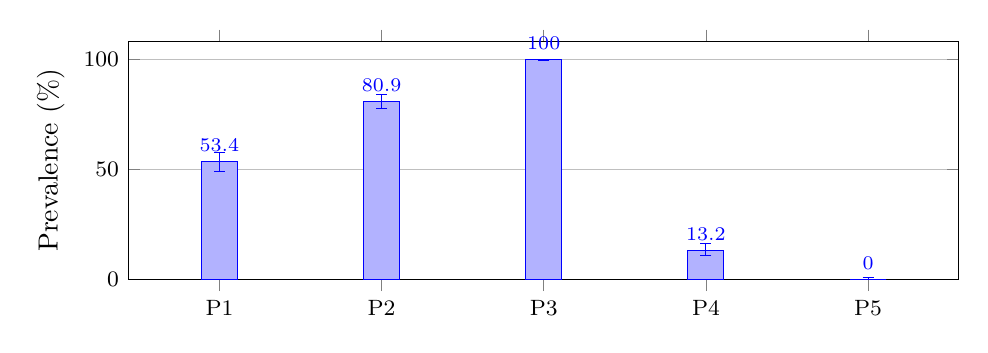
\begin{tikzpicture}
\begin{axis}[
  ybar, bar width=13pt,
  width=\linewidth, height=4.6cm,
  ymin=0, ymax=108, ylabel={Prevalence (\%)},
  symbolic x coords={P1,P2,P3,P4,P5},
  xtick=data, enlarge x limits=0.14,
  nodes near coords, nodes near coords align={vertical},
  every node near coord/.append style={font=\scriptsize},
  ymajorgrids, tick label style={font=\footnotesize},
]
% asymmetric explicit errors:  += (0, upper)  -= (0, lower)
\addplot+[error bars/.cd, y dir=both, y explicit]
coordinates {
  (P1,53.4)  += (0,4.2)  -= (0,4.3)
  (P2,80.9)  += (0,3.2)  -= (0,3.5)
  (P3,100.0) += (0,0.0)  -= (0,0.7)
  (P4,13.2)  += (0,3.2)  -= (0,2.6)
  (P5,0.0)   += (0,0.7)  -= (0,0.0)
};
\end{axis}
\end{tikzpicture}
\caption{Prevalence of cited verification weaknesses across 530 distinct
JWT-validating configurations, with Wilson 95\% confidence intervals.
P1 unbound audience; P2 no required claims; P3 no algorithm pinning \emph{in
configuration} (library-default caveat, \S\ref{sec:results}); P4 multi-issuer
(descriptive); P5 clock skew $>5$\,min (now read from Envoy
\texttt{clock\_skew\_seconds}; the widest observed is 60\,s). An independently
validated extractor; a hand-labelled gold standard is still pending
(\S\ref{sec:limitations}).}
\label{fig:prevalence}
\end{figure}

\noindent\textbf{Drift (RQ: how contracts change over time).}
Longitudinal analysis over commit history is future work. Today we validate the
drift \emph{classifier} on a 1{,}226-pair synthetic corpus at 100\% recall / 0\%
FPR, with mutation testing (24 mutants, 100\% killed) and a held-out adversarial
set at Youden 0.75. \gate{Drift in the wild, over real commit histories, is left to
the full study.}

\section{Limitations and threats to validity}\label{sec:limitations}
\textbf{Declared, not effective.} We measure the contract configuration declares,
not what the running verifier enforces. A configured check can still be skipped by
buggy verifier code, and a check absent from configuration can still hold because a
library default supplies it; conversely an implementation flaw (accepting
\texttt{alg=none}, RS/HS confusion) is invisible to us. We therefore report an
absent check as ``not set in configuration,'' not as a confirmed vulnerability, and
closing this gap needs live probing or a library-defaults database, which we leave
to future work. \textbf{Profile dependence.} Which checks are mandatory depends on
the token profile: audience and issuer validation are required for RFC~9068 access
tokens but optional for a bare RFC~7519 JWT, so an ``unbound audience'' is a
weakness only under a profile that requires binding; we measure the configured check
and name the profile where the corpus reveals it. \textbf{Templating:} $\approx$13\% of corpus files are
Helm-templated and $\approx$8\% carry kustomize/variable markers, so roughly one in
five configurations is under-resolved without rendering. \textbf{Selection bias:}
public configuration skews to samples, demos, and OSS and is not representative of
private enterprise deployments; this must be stated, not hidden. \textbf{Proxy
oracles:} \S\ref{sec:validation}'s recall/precision are automated approximations
pending human labels. \textbf{Ethics:} we use only public configuration, read
only; we do not probe third-party live endpoints and handle no real tokens;
identifiable high-severity findings follow responsible disclosure.

\section{Related work}\label{sec:related}
\noindent\textbf{In-the-wild web-authentication and SSO measurement.} The closest
line of work measures deployed authentication. Early studies inspect a small set of
sites by hand and show that SSO and OAuth failures are driven by deployment and
implementation choices rather than protocol flaws~\cite{authzmeas2012wangsignmein,authzmeas2012sunoauth}.
Later work makes this a population measurement: SSOScan automatically tests a fixed
catalog of five SSO vulnerabilities across the top 20{,}000 sites and finds that over
20\% of Facebook-SSO sites carry a serious flaw~\cite{authzmeas2014ssoscan}, and
subsequent studies measure sign-off and session handling, dual-window SSO, and SSO
adoption across the Tranco list~\cite{authzmeas2018singlesignoff,authzmeas2022distinct,authzmeas2023ssomonitor};
the OpenID Connect attack classes are systematized by Mainka et al.~\cite{authzmeas2017soksso}.
SSOScan is our closest methodological ancestor: automated detection of a fixed
weakness catalog over a crawled population. We keep that ambition but change the
object and the vantage point. We read the declared verification contract out of
static mesh and proxy configuration rather than driving a runtime login flow, which
reaches services no crawler can log into and separates what a service declares from
what it enforces.

\noindent\textbf{Large-scale misconfiguration measurement.} Our methodology follows
a well-established template: crawl a population, report the prevalence of a concrete
weakness, and quantify uncertainty. Studies of the HTTPS certificate ecosystem and
of Heartbleed turn repeated scans into a structured prevalence
picture~\cite{authzmeas2013httpsecosystem,authzmeas2014heartbleed}; the email-delivery
study measures adoption of \emph{declared} security policies (SPF, DKIM, DMARC)
across more than 700{,}000 servers~\cite{authzmeas2015emaildelivery}; and studies of
HTTPS adoption, Content Security Policy, CORS, and S3 buckets measure how a declared
per-service policy is set or fails at scale~\cite{authzmeas2017httpsadoption,authzmeas2016csp,authzmeas2018cors,authzmeas2018s3buckets}.
We adopt this template, including confidence intervals and a replication-style
validation of recall and precision, and apply it to a surface none of these touch,
the JWT authorization contract.

\noindent\textbf{IaC and configuration security.} Repository-mining studies quantify
security weaknesses in declarative infrastructure code: the Seven Sins study derives
smells from 1{,}726 scripts and counts occurrences across hundreds of
repositories~\cite{authzmeas2019sevensins}, replicated at larger scale and across
technologies~\cite{authzmeas2021iacreplication,authzmeas2022glitch}, and Kubernetes
security practice is systematized separately~\cite{authzmeas2020k8scommandments}.
Practitioner scanners (Checkov, KICS, Terrascan, Semgrep) and policy-as-code
engines~\cite{authzmeas2024checkov,authzmeas2024kics,authzmeas2024terrascan,authzmeas2024semgrep,authzmeas2024opa}
apply rule sets to individual files. These target generic hygiene (hard-coded
secrets, weak crypto) and check rules per file; we instead normalize heterogeneous
mesh and proxy configuration into one typed authorization contract per service and
measure its properties, and our negative control targets the attribution errors that
per-file pattern-matching is prone to.

\noindent\textbf{Formal analysis and config-as-contract.} A body of formal and
attack analysis establishes \emph{which} issuer, audience, algorithm, and endpoint
behaviours are load-bearing, for SAML, OAuth, and OpenID
Connect~\cite{authzmeas2008samlsso,authzmeas2012websanalysis,authzmeas2016oauthformal,authzmeas2017oidcformal};
the concrete JWT weaknesses we count (\texttt{alg=none}, RS/HS key confusion) are
documented by practitioners~\cite{authzmeas2015jwtlibs,authzmeas2024portswiggerjwt}
and codified in RFC~8725~\cite{rfc8725}. We cite these for the properties and then
measure how often deployments violate them rather than re-arguing relevance. The
idea of deriving a policy model from static configuration has a precedent in Batfish,
which parses heterogeneous device configuration into a vendor-independent model and
checks properties over it~\cite{authzmeas2015batfish}, and in ABAC policy
mining~\cite{authzmeas2015abacmining}; consumer-driven contract testing (Pact) shares
the ``contract'' framing~\cite{authzmeas2024pact}. None recovers a JWT authorization
contract or measures one across a population.

\noindent\textbf{Agent and MCP authorization.} Indirect prompt injection makes
token-scoped, verifiable authorization necessary for autonomous
agents~\cite{authzmeas2023promptinjection}, and recent measurements of live remote
MCP servers report widespread missing authentication and OAuth
flaws~\cite{authzmeas2026mcpauthmeas,authzmeas2026mcpexposed}. These show the same
population-measurement method reaching the agent frontier, where the declared-versus-effective
contract framing of this paper is the natural lens to carry forward.

\section{Future work}\label{sec:future}
Three extensions follow directly. (i) Pairing the static reading with live probing
would close the declared-vs-effective gap this paper is careful to leave open,
turning ``not set in configuration'' into a confirmed runtime behaviour. (ii) The
content-addressed contract makes \emph{drift} measurable over commit history: do
contracts widen more than they narrow, and are widenings tied to reviewable events?
(iii) The same instrument extends to the agent and MCP frontier, where OAuth/MCP
tokens carry the same issuer, audience, and claim checks on a faster-moving surface.

\section{Conclusion}
A service's decision to accept a token is configuration, declared across meshes,
proxies, and identity providers and rarely collected in one place. We make that
declared authorization contract an object that can be derived, measured, versioned,
and validated, we separate it from the effective enforcement that configuration
cannot show, and we measure it across 2{,}718 repositories with a methodology
honest about its own limits. The instrument and corpus are released so the
measurement is reproducible and extensible.

\section*{Ethics considerations}\label{sec:ethics}
This study measures only \emph{public} configuration, fetched read-only at pinned
commits, and never probes third-party live endpoints or handles real tokens; the
attack surface it characterises is exercised only against local, self-owned
negative-control fixtures. We report \emph{population} prevalence, never a verdict
on any single project, and we name no project as insecure. For any identifiable,
high-severity finding tied to a specific owner we follow coordinated responsible
disclosure before publication, allowing reasonable remediation time. The corpus
respects source licences (recorded per artifact) and robots/rate-limit norms of the
hosting platform. We see no human-subjects concerns; no personal data is collected.

\section*{Open science}\label{sec:openscience}
In keeping with open-science expectations, we release the discovery instrument, the
measurement harness (prevalence with Wilson CIs), the kind-aware validator, the
non-circular negative-control precision test, the analysis scripts, and the corpus
\emph{manifest} (repository + commit SHA + licence per artifact) so the measurement
is reproducible from public sources. \gate{At camera-ready we will add a DOI-pinned
archival snapshot and, where the venue offers it, Artifact-Evaluation ``Available'' and
``Reproduced'' badges.}

\section*{Artifact availability}\label{sec:artifact}
The instrument, harness, validator, negative-control test, and corpus manifest are
open source under the MIT licence. \gate{The archival DOI will be added at
camera-ready.}
. Every unfinished number is wrapped in \gate{...}.
% Submission vs. working-copy rendering. Default: submission (clean prose). A
% wrapper can predefine \submissionfalse before % Shared body for the Paper A measurement study. Class-agnostic: the per-venue
% main.tex sets \documentclass, title, authors, and \begin{document}, then
% % Shared body for the Paper A measurement study. Class-agnostic: the per-venue
% main.tex sets \documentclass, title, authors, and \begin{document}, then
% \input{../common/body}. Every unfinished number is wrapped in \gate{...}.
% Submission vs. working-copy rendering. Default: submission (clean prose). A
% wrapper can predefine \submissionfalse before \input{../common/body} to bring
% back the loud [PENDING]/[NOTE] markers for internal tracking.
\ifdefined\ifsubmission\else\expandafter\newif\csname ifsubmission\endcsname\submissiontrue\fi
% \gate{...}: forward-looking text. Submission -> plain prose; draft -> [PENDING].
% Content is written to read as a finished future-work sentence either way.
\providecommand{\gate}[1]{\ifsubmission #1\else \textbf{[PENDING: #1]}\fi}
% \draftonly{...}: internal note. Submission -> nothing; draft -> [NOTE].
\providecommand{\draftonly}[1]{\ifsubmission\else \textbf{[NOTE: #1]}\fi}
% Let TeX relax line breaking on paragraphs with long unbreakable \texttt{} kind
% names (RequestAuthentication, AuthorizationPolicy) instead of overrunning the
% margin. Class-agnostic; applies under every venue wrapper.
\emergencystretch=3em

% The abstract lives in common/abstract.tex. acmart requires it BEFORE \maketitle,
% llncs/IEEEtran after, so an acmart wrapper \inputs it itself (and defines
% \keywayabstractdone); every other wrapper lets the body emit it here.
\ifdefined\keywayabstractdone\else\input{abstract}\fi

\section{Introduction}
An engineer rotates a signing key on a Friday. No code changes; every test passes.
By Monday a downstream service is rejecting every valid user, because its verifier
cached the retired key longer than anyone realised. The same week, elsewhere, a
verifier quietly begins accepting a second audience nobody intended. Neither
failure lives in the code, and neither would be caught by reading it: both live in
the \emph{configuration} that actually decides whether a bearer token is accepted.

That configuration is an implicit specification: the issuers a verifier trusts,
the audiences it binds to, the algorithms it allows, the claims it requires, and
the JWKS behaviour of the library beneath it. We call it the \emph{authorization
contract}. It is spread across service meshes, proxies, identity providers, and
library defaults, it is almost never centralised, and it \emph{drifts}: a rotated
key, a widened audience, or a dropped claim turns valid users away (an outage) or
admits tokens that should be refused (a silent regression). As autonomous agents
begin carrying OAuth/MCP tokens on a user's behalf, the same contract now governs a
faster-moving, higher-stakes surface.

A caveat shapes the whole paper. What configuration states is the \emph{declared}
contract; whether a request is ultimately accepted is the \emph{effective}
behaviour, which also depends on the verifier's code, its library's defaults, and
its software version. A verifier may, for example, accept the \texttt{none}
algorithm because of an implementation flaw even where configuration says nothing,
and that is not visible in configuration at all. We measure the declared contract,
we say so throughout, and \S\ref{sec:background} and \S\ref{sec:limitations} make
the boundary between declared and effective explicit; where a declared value is
absent we distinguish ``not set in configuration'' from ``not enforced.''

This declared contract is where much of auth correctness is decided, and yet almost
nobody measures it at scale. Two kinds of tooling exist and neither answers ``what
do deployed authorization contracts look like across a population, and how healthy
are they?'' Static code scanners reason about source, not about which configured
verifier trusts which issuer; gateways and identity providers are the thing being
configured, so they do not tell an operator whether that configuration is healthy.

\noindent\textbf{Contributions.}
(i) We define the \emph{authorization contract} and give a method that derives it
from heterogeneous deployment configuration (Istio, Envoy, OIDC) with per-field
provenance and content-addressed versioning, separating the declared contract from
effective enforcement (\S\ref{sec:method}).
(ii) We measure how common concrete, normatively grounded weaknesses are across
2{,}718 public repositories and 530 JWT-validating configurations, with confidence
intervals and a co-occurrence analysis (\S\ref{sec:results}).
(iii) We give a validation methodology that is explicit about its own limits:
recall against an independent parse, a non-circular negative control for precision,
and a held-out over-attribution split, each with its failure mode stated
(\S\ref{sec:validation}).
(iv) We release the instrument, the corpus manifest, and the analysis so the study
is reproducible from public sources (\S\ref{sec:artifact}).

\section{Background}\label{sec:background}

\noindent\textbf{JWT verification.} A JSON Web Token is a signed statement of
claims: a header naming the signing algorithm, a payload of claims (including
\texttt{iss}, the issuer; \texttt{aud}, the intended audience; \texttt{exp}, the
expiry), and a signature. To accept a token, a verifier must (1) fetch the issuer's
public keys, in practice from a JSON Web Key Set (JWKS) endpoint, and verify the
signature; (2) check that \texttt{iss} is a trusted issuer; (3) check that
\texttt{aud} names this resource; (4) accept only an allow-list of signing
algorithms; and (5) enforce any additional required claims (roles, scopes, tenant).
Each step has a normative source. RFC~8725 (JSON Web Token Best Current Practices)
requires an explicit algorithm allow-list (\S3.1) and validation of all security
claims (\S3.9); RFC~9068 profiles JWT \emph{access tokens} and makes audience and
issuer validation mandatory for that profile; RFC~8707 (resource indicators) and
RFC~9728 (protected-resource metadata) bind a token to the resource it was minted
for. Which checks are mandatory therefore depends partly on the token profile in
use, a point we return to in \S\ref{sec:limitations}.

\noindent\textbf{Where the contract lives.} Few services implement these checks in
application code. In a service mesh the checks are declared as configuration and
enforced by a sidecar or gateway. Under Istio, a \texttt{RequestAuthentication}
resource declares the issuer, the JWKS source, and the accepted audiences, while an
\texttt{AuthorizationPolicy} declares required claims as \texttt{when} conditions on
\texttt{request.auth.claims[...]}; under Envoy, a \texttt{jwt\_authn} filter carries
the providers, audiences, and clock-skew tolerance. These resources usually live in
\emph{different files}, and the effective contract for one workload is their union.
Figure~\ref{fig:example} shows a minimal pair.

\begin{figure}[t]
\footnotesize
\begin{verbatim}
kind: RequestAuthentication      # issuer + audience
spec:
  selector: {matchLabels: {app: orders}}
  jwtRules:
  - issuer: "https://idp.example/realms/main"
    jwksUri: "https://idp.example/jwks.json"
    audiences: ["orders-api"]
---
kind: AuthorizationPolicy        # a required claim
spec:
  selector: {matchLabels: {app: orders}}
  rules:
  - when:
    - key: request.auth.claims[groups]
      values: ["ops"]
\end{verbatim}
\caption{The declared authorization contract for the \texttt{orders} workload,
spread across two resources: trust \texttt{idp.example}, require audience
\texttt{orders-api}, and require a \texttt{groups} claim of \texttt{ops}. No signing
algorithm is pinned, so the mesh applies its library default (\S\ref{sec:results}).}
\label{fig:example}
\end{figure}

\noindent\textbf{Declared vs.\ effective; terminology.} We measure the
\emph{declared} contract in resources like these. The \emph{effective} behaviour
can differ: a verifier might skip a check, honour a dangerous default, or carry an
implementation bug (accepting \texttt{alg=none}, confusing RS256 and HS256). Those
are code, not configuration, and outside the reach of a static reading; we flag the
absence of a configured check as ``not set in configuration,'' never as a confirmed
runtime vulnerability. We use \emph{consumer} for the verifying entity a contract
belongs to (an Istio workload, an Envoy route), and we restrict \emph{authorization
contract} to \emph{token validation} (is this token acceptable?), as distinct from
resource-level authorization (may this subject perform this action?), which is a
separate layer we do not measure.

\section{Deriving authorization contracts}\label{sec:method}
We derive one contract per \emph{consumer} (\S\ref{sec:background}) from the
configuration that governs it. Source-specific \emph{discoverers} parse each format
(Istio \texttt{RequestAuthentication} and \texttt{AuthorizationPolicy}, Envoy
\texttt{jwt\_authn}, and OIDC/Keycloak registries) into a common contract of
issuers, audiences, algorithms, required claims, and JWKS behaviour.

Deriving a contract is not a one-resource read, because the checks are split across
resources (\S\ref{sec:background}). For the pair in Figure~\ref{fig:example}, the
\texttt{RequestAuthentication} contributes the issuer, JWKS source, and audience,
and the \texttt{AuthorizationPolicy} contributes the required \texttt{groups} claim;
we join them by the workload they select (\texttt{app: orders}) into a single
consumer whose contract carries all three. Attribution follows the mesh's own
semantics: a selector-less policy applies to every workload in its namespace, and
in a namespace with a single JWT consumer a per-service claim policy attaches to
that consumer (the common edge-gateway pattern). The same join resolves audiences
declared in an \texttt{AuthorizationPolicy} condition on
\texttt{request.auth.audiences} rather than in the \texttt{RequestAuthentication}.

Every extracted field records \emph{provenance}: the source kind, the file
locator, and a confidence. Each measurement is therefore attributable to a line of
configuration and a human can check it (we use this in \S\ref{sec:validation}).
A library-defaults database records what a verifier does when configuration is
silent, kept separate from what configuration states so the two are never conflated.
Consumers are assembled into a content-addressed \texttt{ContractVersion}, which
makes change detection exact equality and lets us diff one deployment's contract
against another or against its own history.

\section{Corpus construction}\label{sec:corpus}
We crawl public GitHub read-only for real auth configuration (Istio
\texttt{RequestAuthentication}, Envoy \texttt{jwt\_authn}, Istio claim conditions),
recording repository, blob SHA, and licence for every artifact for reproducibility
and attribution. We fetch public repositories only, cap files per repository to
limit monorepo dominance, and analyse \emph{per repository} so a
\texttt{RequestAuthentication} and its \texttt{AuthorizationPolicy} (usually in
separate files) are resolved together while distinct repositories remain isolated.
Two cleaning steps address representativeness: we exclude tutorial/vendored copies
by path (matched against the full locator, so \texttt{testdata/}, \texttt{vendor/},
and \texttt{/e2e/} components are caught, not only basenames), and we deduplicate
identical configurations (a canonical sample pasted across repositories counts
once). The corpus is 5{,}214 files across 2{,}718 public repositories, yielding 778
JWT-validating configurations, or 530 after deduplication. \gate{A full study will
push the corpus further toward $10^4$ services, add OIDC/MCP sources, and report a
selection-bias analysis against the public-configuration population.}

\section{Validation methodology}\label{sec:validation}
Measurement is only as good as the extractor. We validate discovery three ways, for
recall, for precision, and for over-attribution, and are explicit about what each
can and cannot establish.

\noindent\textbf{Recall (kind-aware independent parse).} An independent YAML parse
of each repository yields the declared issuers/audiences/claims; we compare to what
discovery captured, per repository. The independent parser also
\emph{over-declares}: it scrapes \texttt{issuer:} keys and claim-like strings from
non-auth resources (a ConfigMap, an annotation). We therefore measure recall only
against values in \emph{genuine} auth resources (RequestAuthentication /
AuthorizationPolicy / Envoy JWT). Adjudicated recall is issuers 96.0\%, audiences
98.2\%, and claims 86.0\% (scoped to repositories where a JWT consumer exists;
claims declared in repositories whose RequestAuthentication is absent from the
corpus have no consumer to attach to). The adjudication removed 106 parser
over-declarations (65 issuers, 27 audiences, 14 claims), which both raises the
honest recall and demonstrates the proxy oracle is itself imperfect. The issuer
figure rose from an earlier 89.6\% once a document-splitting bug was fixed: a single
templated or malformed YAML document had been aborting the rest of its file, so the
earlier recall was depressed by the extractor, not by the corpus.

\noindent\textbf{Precision (non-circular negative control).} An independent-parse
oracle cannot honestly measure precision: it reads the same fields as the
extractor, so captures are almost always a subset and precision $\approx 100\%$
\emph{by construction}. We therefore use a negative control: configurations with
planted distractor values a correct discoverer must ignore: a commented-out
issuer, an \texttt{issuer:}/claim in a non-auth ConfigMap, a claim behind a
non-matching AuthorizationPolicy selector (the real attribution risk), and strings
in annotations. Result: 4 planted, 0 leaked, with real values still captured.

\noindent\textbf{Over-attribution (held-out split).} To measure how often discovery
\emph{adds} a value that is not really there, we take every captured/declared
disagreement, label each with an independent model that reads only the raw
configuration and never the extractor's output (so the grading is non-circular),
and split the labelled set 70/30 by repository so no repository informs both sides.
On the held-out test split, precision is 100\% and over-attribution is 0.0\% (0 of 6
captured-only values are spurious or mis-attributed); on the full labelled set,
precision 100\% and over-attribution 0.0\%. This split is what caught, and then
confirmed the fix for, an Envoy test-fixture leak and a claim mis-attribution during
development.

\noindent\textbf{Gold standard.} All three above are automated or model-assisted
proxies. For a population-level ground truth we draw a stratified random sample of
401 \mbox{(repo, field, value)} rows across the corpus, powered for a $\pm$1.8\%
precision and $\pm$2.4\% recall confidence interval, and have each adjudicated by
hand as real, correctly attributed, or spurious; a model drafts a first-pass label
that the human confirms or corrects, and a blind subset gives an un-anchored
inter-annotator agreement (Cohen's $\kappa$). \gate{We report the hand-validated
precision, recall, and $\kappa$ in the final version; the automated results above
are what the gold standard refines.}

\section{Results}\label{sec:results}
We report prevalence over the 530 deduplicated JWT-validating configurations, each
with a 95\% Wilson confidence interval (the Wilson interval is preferred over the
normal approximation for proportions near 0 or 1). These figures come from the
independently validated extractor of \S\ref{sec:validation}; the hand-validated
gold standard refines the \emph{validation} numbers, not the prevalence below.

\noindent\textbf{Prevalence.} Over 530 distinct JWT-validating configurations
(Wilson 95\% CIs): no algorithm pinning \emph{in configuration} 100\%
[99.3, 100]; no required claims 80.9\% [77.4, 84.1]; unbound audience 53.4\%
[49.1, 57.6]; multi-issuer trust 13.2\% [10.6, 16.4] (descriptive, not a weakness);
clock skew $>5$\,min 0.0\% [0.0, 0.7]. The algorithm-pinning figure reflects
reliance on the verifying \emph{library's default}, which configuration does not
restate. This is a static-vs-runtime gap, not a 100\% vulnerability rate; we report
it as ``not pinned in config.'' The clock-skew figure is now read directly from
Envoy \texttt{clock\_skew\_seconds} rather than assumed: of the configurations that
set it the widest is 60\,s, so the 0.0\% above the 5-minute threshold is measured,
not merely unobserved. The earlier draft's 42.2\% unbound-audience figure, over a
102-configuration pilot, rises to 53.4\% on this larger and more representative
corpus; the direction and the majority finding are unchanged.

\noindent\textbf{Co-occurrence.} Weaknesses travel together. No-required-claims and
no-algorithm-pinning co-occur in 80.9\% of configurations; unbound-audience with
no-algorithm-pinning in 53.4\%; unbound-audience with no-required-claims in 43.8\%
(lift $\approx$1.0, i.e. roughly independent rather than mutually reinforcing).

\noindent\textbf{Static/runtime frontier.} Four of the five check types are
conclusive from configuration alone; only algorithm pinning carries the
library-default caveat. Of 1{,}312 weakness flags raised, 782 (60\%) are
static-conclusive and 530 carry that caveat, quantifying how much of the contract a
purely static reading can settle.

\input{../common/fig-prevalence}

\noindent\textbf{Drift (RQ: how contracts change over time).}
Longitudinal analysis over commit history is future work. Today we validate the
drift \emph{classifier} on a 1{,}226-pair synthetic corpus at 100\% recall / 0\%
FPR, with mutation testing (24 mutants, 100\% killed) and a held-out adversarial
set at Youden 0.75. \gate{Drift in the wild, over real commit histories, is left to
the full study.}

\section{Limitations and threats to validity}\label{sec:limitations}
\textbf{Declared, not effective.} We measure the contract configuration declares,
not what the running verifier enforces. A configured check can still be skipped by
buggy verifier code, and a check absent from configuration can still hold because a
library default supplies it; conversely an implementation flaw (accepting
\texttt{alg=none}, RS/HS confusion) is invisible to us. We therefore report an
absent check as ``not set in configuration,'' not as a confirmed vulnerability, and
closing this gap needs live probing or a library-defaults database, which we leave
to future work. \textbf{Profile dependence.} Which checks are mandatory depends on
the token profile: audience and issuer validation are required for RFC~9068 access
tokens but optional for a bare RFC~7519 JWT, so an ``unbound audience'' is a
weakness only under a profile that requires binding; we measure the configured check
and name the profile where the corpus reveals it. \textbf{Templating:} $\approx$13\% of corpus files are
Helm-templated and $\approx$8\% carry kustomize/variable markers, so roughly one in
five configurations is under-resolved without rendering. \textbf{Selection bias:}
public configuration skews to samples, demos, and OSS and is not representative of
private enterprise deployments; this must be stated, not hidden. \textbf{Proxy
oracles:} \S\ref{sec:validation}'s recall/precision are automated approximations
pending human labels. \textbf{Ethics:} we use only public configuration, read
only; we do not probe third-party live endpoints and handle no real tokens;
identifiable high-severity findings follow responsible disclosure.

\section{Related work}\label{sec:related}
\noindent\textbf{In-the-wild web-authentication and SSO measurement.} The closest
line of work measures deployed authentication. Early studies inspect a small set of
sites by hand and show that SSO and OAuth failures are driven by deployment and
implementation choices rather than protocol flaws~\cite{authzmeas2012wangsignmein,authzmeas2012sunoauth}.
Later work makes this a population measurement: SSOScan automatically tests a fixed
catalog of five SSO vulnerabilities across the top 20{,}000 sites and finds that over
20\% of Facebook-SSO sites carry a serious flaw~\cite{authzmeas2014ssoscan}, and
subsequent studies measure sign-off and session handling, dual-window SSO, and SSO
adoption across the Tranco list~\cite{authzmeas2018singlesignoff,authzmeas2022distinct,authzmeas2023ssomonitor};
the OpenID Connect attack classes are systematized by Mainka et al.~\cite{authzmeas2017soksso}.
SSOScan is our closest methodological ancestor: automated detection of a fixed
weakness catalog over a crawled population. We keep that ambition but change the
object and the vantage point. We read the declared verification contract out of
static mesh and proxy configuration rather than driving a runtime login flow, which
reaches services no crawler can log into and separates what a service declares from
what it enforces.

\noindent\textbf{Large-scale misconfiguration measurement.} Our methodology follows
a well-established template: crawl a population, report the prevalence of a concrete
weakness, and quantify uncertainty. Studies of the HTTPS certificate ecosystem and
of Heartbleed turn repeated scans into a structured prevalence
picture~\cite{authzmeas2013httpsecosystem,authzmeas2014heartbleed}; the email-delivery
study measures adoption of \emph{declared} security policies (SPF, DKIM, DMARC)
across more than 700{,}000 servers~\cite{authzmeas2015emaildelivery}; and studies of
HTTPS adoption, Content Security Policy, CORS, and S3 buckets measure how a declared
per-service policy is set or fails at scale~\cite{authzmeas2017httpsadoption,authzmeas2016csp,authzmeas2018cors,authzmeas2018s3buckets}.
We adopt this template, including confidence intervals and a replication-style
validation of recall and precision, and apply it to a surface none of these touch,
the JWT authorization contract.

\noindent\textbf{IaC and configuration security.} Repository-mining studies quantify
security weaknesses in declarative infrastructure code: the Seven Sins study derives
smells from 1{,}726 scripts and counts occurrences across hundreds of
repositories~\cite{authzmeas2019sevensins}, replicated at larger scale and across
technologies~\cite{authzmeas2021iacreplication,authzmeas2022glitch}, and Kubernetes
security practice is systematized separately~\cite{authzmeas2020k8scommandments}.
Practitioner scanners (Checkov, KICS, Terrascan, Semgrep) and policy-as-code
engines~\cite{authzmeas2024checkov,authzmeas2024kics,authzmeas2024terrascan,authzmeas2024semgrep,authzmeas2024opa}
apply rule sets to individual files. These target generic hygiene (hard-coded
secrets, weak crypto) and check rules per file; we instead normalize heterogeneous
mesh and proxy configuration into one typed authorization contract per service and
measure its properties, and our negative control targets the attribution errors that
per-file pattern-matching is prone to.

\noindent\textbf{Formal analysis and config-as-contract.} A body of formal and
attack analysis establishes \emph{which} issuer, audience, algorithm, and endpoint
behaviours are load-bearing, for SAML, OAuth, and OpenID
Connect~\cite{authzmeas2008samlsso,authzmeas2012websanalysis,authzmeas2016oauthformal,authzmeas2017oidcformal};
the concrete JWT weaknesses we count (\texttt{alg=none}, RS/HS key confusion) are
documented by practitioners~\cite{authzmeas2015jwtlibs,authzmeas2024portswiggerjwt}
and codified in RFC~8725~\cite{rfc8725}. We cite these for the properties and then
measure how often deployments violate them rather than re-arguing relevance. The
idea of deriving a policy model from static configuration has a precedent in Batfish,
which parses heterogeneous device configuration into a vendor-independent model and
checks properties over it~\cite{authzmeas2015batfish}, and in ABAC policy
mining~\cite{authzmeas2015abacmining}; consumer-driven contract testing (Pact) shares
the ``contract'' framing~\cite{authzmeas2024pact}. None recovers a JWT authorization
contract or measures one across a population.

\noindent\textbf{Agent and MCP authorization.} Indirect prompt injection makes
token-scoped, verifiable authorization necessary for autonomous
agents~\cite{authzmeas2023promptinjection}, and recent measurements of live remote
MCP servers report widespread missing authentication and OAuth
flaws~\cite{authzmeas2026mcpauthmeas,authzmeas2026mcpexposed}. These show the same
population-measurement method reaching the agent frontier, where the declared-versus-effective
contract framing of this paper is the natural lens to carry forward.

\section{Future work}\label{sec:future}
Three extensions follow directly. (i) Pairing the static reading with live probing
would close the declared-vs-effective gap this paper is careful to leave open,
turning ``not set in configuration'' into a confirmed runtime behaviour. (ii) The
content-addressed contract makes \emph{drift} measurable over commit history: do
contracts widen more than they narrow, and are widenings tied to reviewable events?
(iii) The same instrument extends to the agent and MCP frontier, where OAuth/MCP
tokens carry the same issuer, audience, and claim checks on a faster-moving surface.

\section{Conclusion}
A service's decision to accept a token is configuration, declared across meshes,
proxies, and identity providers and rarely collected in one place. We make that
declared authorization contract an object that can be derived, measured, versioned,
and validated, we separate it from the effective enforcement that configuration
cannot show, and we measure it across 2{,}718 repositories with a methodology
honest about its own limits. The instrument and corpus are released so the
measurement is reproducible and extensible.

\section*{Ethics considerations}\label{sec:ethics}
This study measures only \emph{public} configuration, fetched read-only at pinned
commits, and never probes third-party live endpoints or handles real tokens; the
attack surface it characterises is exercised only against local, self-owned
negative-control fixtures. We report \emph{population} prevalence, never a verdict
on any single project, and we name no project as insecure. For any identifiable,
high-severity finding tied to a specific owner we follow coordinated responsible
disclosure before publication, allowing reasonable remediation time. The corpus
respects source licences (recorded per artifact) and robots/rate-limit norms of the
hosting platform. We see no human-subjects concerns; no personal data is collected.

\section*{Open science}\label{sec:openscience}
In keeping with open-science expectations, we release the discovery instrument, the
measurement harness (prevalence with Wilson CIs), the kind-aware validator, the
non-circular negative-control precision test, the analysis scripts, and the corpus
\emph{manifest} (repository + commit SHA + licence per artifact) so the measurement
is reproducible from public sources. \gate{At camera-ready we will add a DOI-pinned
archival snapshot and, where the venue offers it, Artifact-Evaluation ``Available'' and
``Reproduced'' badges.}

\section*{Artifact availability}\label{sec:artifact}
The instrument, harness, validator, negative-control test, and corpus manifest are
open source under the MIT licence. \gate{The archival DOI will be added at
camera-ready.}
. Every unfinished number is wrapped in \gate{...}.
% Submission vs. working-copy rendering. Default: submission (clean prose). A
% wrapper can predefine \submissionfalse before % Shared body for the Paper A measurement study. Class-agnostic: the per-venue
% main.tex sets \documentclass, title, authors, and \begin{document}, then
% \input{../common/body}. Every unfinished number is wrapped in \gate{...}.
% Submission vs. working-copy rendering. Default: submission (clean prose). A
% wrapper can predefine \submissionfalse before \input{../common/body} to bring
% back the loud [PENDING]/[NOTE] markers for internal tracking.
\ifdefined\ifsubmission\else\expandafter\newif\csname ifsubmission\endcsname\submissiontrue\fi
% \gate{...}: forward-looking text. Submission -> plain prose; draft -> [PENDING].
% Content is written to read as a finished future-work sentence either way.
\providecommand{\gate}[1]{\ifsubmission #1\else \textbf{[PENDING: #1]}\fi}
% \draftonly{...}: internal note. Submission -> nothing; draft -> [NOTE].
\providecommand{\draftonly}[1]{\ifsubmission\else \textbf{[NOTE: #1]}\fi}
% Let TeX relax line breaking on paragraphs with long unbreakable \texttt{} kind
% names (RequestAuthentication, AuthorizationPolicy) instead of overrunning the
% margin. Class-agnostic; applies under every venue wrapper.
\emergencystretch=3em

% The abstract lives in common/abstract.tex. acmart requires it BEFORE \maketitle,
% llncs/IEEEtran after, so an acmart wrapper \inputs it itself (and defines
% \keywayabstractdone); every other wrapper lets the body emit it here.
\ifdefined\keywayabstractdone\else\input{abstract}\fi

\section{Introduction}
An engineer rotates a signing key on a Friday. No code changes; every test passes.
By Monday a downstream service is rejecting every valid user, because its verifier
cached the retired key longer than anyone realised. The same week, elsewhere, a
verifier quietly begins accepting a second audience nobody intended. Neither
failure lives in the code, and neither would be caught by reading it: both live in
the \emph{configuration} that actually decides whether a bearer token is accepted.

That configuration is an implicit specification: the issuers a verifier trusts,
the audiences it binds to, the algorithms it allows, the claims it requires, and
the JWKS behaviour of the library beneath it. We call it the \emph{authorization
contract}. It is spread across service meshes, proxies, identity providers, and
library defaults, it is almost never centralised, and it \emph{drifts}: a rotated
key, a widened audience, or a dropped claim turns valid users away (an outage) or
admits tokens that should be refused (a silent regression). As autonomous agents
begin carrying OAuth/MCP tokens on a user's behalf, the same contract now governs a
faster-moving, higher-stakes surface.

A caveat shapes the whole paper. What configuration states is the \emph{declared}
contract; whether a request is ultimately accepted is the \emph{effective}
behaviour, which also depends on the verifier's code, its library's defaults, and
its software version. A verifier may, for example, accept the \texttt{none}
algorithm because of an implementation flaw even where configuration says nothing,
and that is not visible in configuration at all. We measure the declared contract,
we say so throughout, and \S\ref{sec:background} and \S\ref{sec:limitations} make
the boundary between declared and effective explicit; where a declared value is
absent we distinguish ``not set in configuration'' from ``not enforced.''

This declared contract is where much of auth correctness is decided, and yet almost
nobody measures it at scale. Two kinds of tooling exist and neither answers ``what
do deployed authorization contracts look like across a population, and how healthy
are they?'' Static code scanners reason about source, not about which configured
verifier trusts which issuer; gateways and identity providers are the thing being
configured, so they do not tell an operator whether that configuration is healthy.

\noindent\textbf{Contributions.}
(i) We define the \emph{authorization contract} and give a method that derives it
from heterogeneous deployment configuration (Istio, Envoy, OIDC) with per-field
provenance and content-addressed versioning, separating the declared contract from
effective enforcement (\S\ref{sec:method}).
(ii) We measure how common concrete, normatively grounded weaknesses are across
2{,}718 public repositories and 530 JWT-validating configurations, with confidence
intervals and a co-occurrence analysis (\S\ref{sec:results}).
(iii) We give a validation methodology that is explicit about its own limits:
recall against an independent parse, a non-circular negative control for precision,
and a held-out over-attribution split, each with its failure mode stated
(\S\ref{sec:validation}).
(iv) We release the instrument, the corpus manifest, and the analysis so the study
is reproducible from public sources (\S\ref{sec:artifact}).

\section{Background}\label{sec:background}

\noindent\textbf{JWT verification.} A JSON Web Token is a signed statement of
claims: a header naming the signing algorithm, a payload of claims (including
\texttt{iss}, the issuer; \texttt{aud}, the intended audience; \texttt{exp}, the
expiry), and a signature. To accept a token, a verifier must (1) fetch the issuer's
public keys, in practice from a JSON Web Key Set (JWKS) endpoint, and verify the
signature; (2) check that \texttt{iss} is a trusted issuer; (3) check that
\texttt{aud} names this resource; (4) accept only an allow-list of signing
algorithms; and (5) enforce any additional required claims (roles, scopes, tenant).
Each step has a normative source. RFC~8725 (JSON Web Token Best Current Practices)
requires an explicit algorithm allow-list (\S3.1) and validation of all security
claims (\S3.9); RFC~9068 profiles JWT \emph{access tokens} and makes audience and
issuer validation mandatory for that profile; RFC~8707 (resource indicators) and
RFC~9728 (protected-resource metadata) bind a token to the resource it was minted
for. Which checks are mandatory therefore depends partly on the token profile in
use, a point we return to in \S\ref{sec:limitations}.

\noindent\textbf{Where the contract lives.} Few services implement these checks in
application code. In a service mesh the checks are declared as configuration and
enforced by a sidecar or gateway. Under Istio, a \texttt{RequestAuthentication}
resource declares the issuer, the JWKS source, and the accepted audiences, while an
\texttt{AuthorizationPolicy} declares required claims as \texttt{when} conditions on
\texttt{request.auth.claims[...]}; under Envoy, a \texttt{jwt\_authn} filter carries
the providers, audiences, and clock-skew tolerance. These resources usually live in
\emph{different files}, and the effective contract for one workload is their union.
Figure~\ref{fig:example} shows a minimal pair.

\begin{figure}[t]
\footnotesize
\begin{verbatim}
kind: RequestAuthentication      # issuer + audience
spec:
  selector: {matchLabels: {app: orders}}
  jwtRules:
  - issuer: "https://idp.example/realms/main"
    jwksUri: "https://idp.example/jwks.json"
    audiences: ["orders-api"]
---
kind: AuthorizationPolicy        # a required claim
spec:
  selector: {matchLabels: {app: orders}}
  rules:
  - when:
    - key: request.auth.claims[groups]
      values: ["ops"]
\end{verbatim}
\caption{The declared authorization contract for the \texttt{orders} workload,
spread across two resources: trust \texttt{idp.example}, require audience
\texttt{orders-api}, and require a \texttt{groups} claim of \texttt{ops}. No signing
algorithm is pinned, so the mesh applies its library default (\S\ref{sec:results}).}
\label{fig:example}
\end{figure}

\noindent\textbf{Declared vs.\ effective; terminology.} We measure the
\emph{declared} contract in resources like these. The \emph{effective} behaviour
can differ: a verifier might skip a check, honour a dangerous default, or carry an
implementation bug (accepting \texttt{alg=none}, confusing RS256 and HS256). Those
are code, not configuration, and outside the reach of a static reading; we flag the
absence of a configured check as ``not set in configuration,'' never as a confirmed
runtime vulnerability. We use \emph{consumer} for the verifying entity a contract
belongs to (an Istio workload, an Envoy route), and we restrict \emph{authorization
contract} to \emph{token validation} (is this token acceptable?), as distinct from
resource-level authorization (may this subject perform this action?), which is a
separate layer we do not measure.

\section{Deriving authorization contracts}\label{sec:method}
We derive one contract per \emph{consumer} (\S\ref{sec:background}) from the
configuration that governs it. Source-specific \emph{discoverers} parse each format
(Istio \texttt{RequestAuthentication} and \texttt{AuthorizationPolicy}, Envoy
\texttt{jwt\_authn}, and OIDC/Keycloak registries) into a common contract of
issuers, audiences, algorithms, required claims, and JWKS behaviour.

Deriving a contract is not a one-resource read, because the checks are split across
resources (\S\ref{sec:background}). For the pair in Figure~\ref{fig:example}, the
\texttt{RequestAuthentication} contributes the issuer, JWKS source, and audience,
and the \texttt{AuthorizationPolicy} contributes the required \texttt{groups} claim;
we join them by the workload they select (\texttt{app: orders}) into a single
consumer whose contract carries all three. Attribution follows the mesh's own
semantics: a selector-less policy applies to every workload in its namespace, and
in a namespace with a single JWT consumer a per-service claim policy attaches to
that consumer (the common edge-gateway pattern). The same join resolves audiences
declared in an \texttt{AuthorizationPolicy} condition on
\texttt{request.auth.audiences} rather than in the \texttt{RequestAuthentication}.

Every extracted field records \emph{provenance}: the source kind, the file
locator, and a confidence. Each measurement is therefore attributable to a line of
configuration and a human can check it (we use this in \S\ref{sec:validation}).
A library-defaults database records what a verifier does when configuration is
silent, kept separate from what configuration states so the two are never conflated.
Consumers are assembled into a content-addressed \texttt{ContractVersion}, which
makes change detection exact equality and lets us diff one deployment's contract
against another or against its own history.

\section{Corpus construction}\label{sec:corpus}
We crawl public GitHub read-only for real auth configuration (Istio
\texttt{RequestAuthentication}, Envoy \texttt{jwt\_authn}, Istio claim conditions),
recording repository, blob SHA, and licence for every artifact for reproducibility
and attribution. We fetch public repositories only, cap files per repository to
limit monorepo dominance, and analyse \emph{per repository} so a
\texttt{RequestAuthentication} and its \texttt{AuthorizationPolicy} (usually in
separate files) are resolved together while distinct repositories remain isolated.
Two cleaning steps address representativeness: we exclude tutorial/vendored copies
by path (matched against the full locator, so \texttt{testdata/}, \texttt{vendor/},
and \texttt{/e2e/} components are caught, not only basenames), and we deduplicate
identical configurations (a canonical sample pasted across repositories counts
once). The corpus is 5{,}214 files across 2{,}718 public repositories, yielding 778
JWT-validating configurations, or 530 after deduplication. \gate{A full study will
push the corpus further toward $10^4$ services, add OIDC/MCP sources, and report a
selection-bias analysis against the public-configuration population.}

\section{Validation methodology}\label{sec:validation}
Measurement is only as good as the extractor. We validate discovery three ways, for
recall, for precision, and for over-attribution, and are explicit about what each
can and cannot establish.

\noindent\textbf{Recall (kind-aware independent parse).} An independent YAML parse
of each repository yields the declared issuers/audiences/claims; we compare to what
discovery captured, per repository. The independent parser also
\emph{over-declares}: it scrapes \texttt{issuer:} keys and claim-like strings from
non-auth resources (a ConfigMap, an annotation). We therefore measure recall only
against values in \emph{genuine} auth resources (RequestAuthentication /
AuthorizationPolicy / Envoy JWT). Adjudicated recall is issuers 96.0\%, audiences
98.2\%, and claims 86.0\% (scoped to repositories where a JWT consumer exists;
claims declared in repositories whose RequestAuthentication is absent from the
corpus have no consumer to attach to). The adjudication removed 106 parser
over-declarations (65 issuers, 27 audiences, 14 claims), which both raises the
honest recall and demonstrates the proxy oracle is itself imperfect. The issuer
figure rose from an earlier 89.6\% once a document-splitting bug was fixed: a single
templated or malformed YAML document had been aborting the rest of its file, so the
earlier recall was depressed by the extractor, not by the corpus.

\noindent\textbf{Precision (non-circular negative control).} An independent-parse
oracle cannot honestly measure precision: it reads the same fields as the
extractor, so captures are almost always a subset and precision $\approx 100\%$
\emph{by construction}. We therefore use a negative control: configurations with
planted distractor values a correct discoverer must ignore: a commented-out
issuer, an \texttt{issuer:}/claim in a non-auth ConfigMap, a claim behind a
non-matching AuthorizationPolicy selector (the real attribution risk), and strings
in annotations. Result: 4 planted, 0 leaked, with real values still captured.

\noindent\textbf{Over-attribution (held-out split).} To measure how often discovery
\emph{adds} a value that is not really there, we take every captured/declared
disagreement, label each with an independent model that reads only the raw
configuration and never the extractor's output (so the grading is non-circular),
and split the labelled set 70/30 by repository so no repository informs both sides.
On the held-out test split, precision is 100\% and over-attribution is 0.0\% (0 of 6
captured-only values are spurious or mis-attributed); on the full labelled set,
precision 100\% and over-attribution 0.0\%. This split is what caught, and then
confirmed the fix for, an Envoy test-fixture leak and a claim mis-attribution during
development.

\noindent\textbf{Gold standard.} All three above are automated or model-assisted
proxies. For a population-level ground truth we draw a stratified random sample of
401 \mbox{(repo, field, value)} rows across the corpus, powered for a $\pm$1.8\%
precision and $\pm$2.4\% recall confidence interval, and have each adjudicated by
hand as real, correctly attributed, or spurious; a model drafts a first-pass label
that the human confirms or corrects, and a blind subset gives an un-anchored
inter-annotator agreement (Cohen's $\kappa$). \gate{We report the hand-validated
precision, recall, and $\kappa$ in the final version; the automated results above
are what the gold standard refines.}

\section{Results}\label{sec:results}
We report prevalence over the 530 deduplicated JWT-validating configurations, each
with a 95\% Wilson confidence interval (the Wilson interval is preferred over the
normal approximation for proportions near 0 or 1). These figures come from the
independently validated extractor of \S\ref{sec:validation}; the hand-validated
gold standard refines the \emph{validation} numbers, not the prevalence below.

\noindent\textbf{Prevalence.} Over 530 distinct JWT-validating configurations
(Wilson 95\% CIs): no algorithm pinning \emph{in configuration} 100\%
[99.3, 100]; no required claims 80.9\% [77.4, 84.1]; unbound audience 53.4\%
[49.1, 57.6]; multi-issuer trust 13.2\% [10.6, 16.4] (descriptive, not a weakness);
clock skew $>5$\,min 0.0\% [0.0, 0.7]. The algorithm-pinning figure reflects
reliance on the verifying \emph{library's default}, which configuration does not
restate. This is a static-vs-runtime gap, not a 100\% vulnerability rate; we report
it as ``not pinned in config.'' The clock-skew figure is now read directly from
Envoy \texttt{clock\_skew\_seconds} rather than assumed: of the configurations that
set it the widest is 60\,s, so the 0.0\% above the 5-minute threshold is measured,
not merely unobserved. The earlier draft's 42.2\% unbound-audience figure, over a
102-configuration pilot, rises to 53.4\% on this larger and more representative
corpus; the direction and the majority finding are unchanged.

\noindent\textbf{Co-occurrence.} Weaknesses travel together. No-required-claims and
no-algorithm-pinning co-occur in 80.9\% of configurations; unbound-audience with
no-algorithm-pinning in 53.4\%; unbound-audience with no-required-claims in 43.8\%
(lift $\approx$1.0, i.e. roughly independent rather than mutually reinforcing).

\noindent\textbf{Static/runtime frontier.} Four of the five check types are
conclusive from configuration alone; only algorithm pinning carries the
library-default caveat. Of 1{,}312 weakness flags raised, 782 (60\%) are
static-conclusive and 530 carry that caveat, quantifying how much of the contract a
purely static reading can settle.

\input{../common/fig-prevalence}

\noindent\textbf{Drift (RQ: how contracts change over time).}
Longitudinal analysis over commit history is future work. Today we validate the
drift \emph{classifier} on a 1{,}226-pair synthetic corpus at 100\% recall / 0\%
FPR, with mutation testing (24 mutants, 100\% killed) and a held-out adversarial
set at Youden 0.75. \gate{Drift in the wild, over real commit histories, is left to
the full study.}

\section{Limitations and threats to validity}\label{sec:limitations}
\textbf{Declared, not effective.} We measure the contract configuration declares,
not what the running verifier enforces. A configured check can still be skipped by
buggy verifier code, and a check absent from configuration can still hold because a
library default supplies it; conversely an implementation flaw (accepting
\texttt{alg=none}, RS/HS confusion) is invisible to us. We therefore report an
absent check as ``not set in configuration,'' not as a confirmed vulnerability, and
closing this gap needs live probing or a library-defaults database, which we leave
to future work. \textbf{Profile dependence.} Which checks are mandatory depends on
the token profile: audience and issuer validation are required for RFC~9068 access
tokens but optional for a bare RFC~7519 JWT, so an ``unbound audience'' is a
weakness only under a profile that requires binding; we measure the configured check
and name the profile where the corpus reveals it. \textbf{Templating:} $\approx$13\% of corpus files are
Helm-templated and $\approx$8\% carry kustomize/variable markers, so roughly one in
five configurations is under-resolved without rendering. \textbf{Selection bias:}
public configuration skews to samples, demos, and OSS and is not representative of
private enterprise deployments; this must be stated, not hidden. \textbf{Proxy
oracles:} \S\ref{sec:validation}'s recall/precision are automated approximations
pending human labels. \textbf{Ethics:} we use only public configuration, read
only; we do not probe third-party live endpoints and handle no real tokens;
identifiable high-severity findings follow responsible disclosure.

\section{Related work}\label{sec:related}
\noindent\textbf{In-the-wild web-authentication and SSO measurement.} The closest
line of work measures deployed authentication. Early studies inspect a small set of
sites by hand and show that SSO and OAuth failures are driven by deployment and
implementation choices rather than protocol flaws~\cite{authzmeas2012wangsignmein,authzmeas2012sunoauth}.
Later work makes this a population measurement: SSOScan automatically tests a fixed
catalog of five SSO vulnerabilities across the top 20{,}000 sites and finds that over
20\% of Facebook-SSO sites carry a serious flaw~\cite{authzmeas2014ssoscan}, and
subsequent studies measure sign-off and session handling, dual-window SSO, and SSO
adoption across the Tranco list~\cite{authzmeas2018singlesignoff,authzmeas2022distinct,authzmeas2023ssomonitor};
the OpenID Connect attack classes are systematized by Mainka et al.~\cite{authzmeas2017soksso}.
SSOScan is our closest methodological ancestor: automated detection of a fixed
weakness catalog over a crawled population. We keep that ambition but change the
object and the vantage point. We read the declared verification contract out of
static mesh and proxy configuration rather than driving a runtime login flow, which
reaches services no crawler can log into and separates what a service declares from
what it enforces.

\noindent\textbf{Large-scale misconfiguration measurement.} Our methodology follows
a well-established template: crawl a population, report the prevalence of a concrete
weakness, and quantify uncertainty. Studies of the HTTPS certificate ecosystem and
of Heartbleed turn repeated scans into a structured prevalence
picture~\cite{authzmeas2013httpsecosystem,authzmeas2014heartbleed}; the email-delivery
study measures adoption of \emph{declared} security policies (SPF, DKIM, DMARC)
across more than 700{,}000 servers~\cite{authzmeas2015emaildelivery}; and studies of
HTTPS adoption, Content Security Policy, CORS, and S3 buckets measure how a declared
per-service policy is set or fails at scale~\cite{authzmeas2017httpsadoption,authzmeas2016csp,authzmeas2018cors,authzmeas2018s3buckets}.
We adopt this template, including confidence intervals and a replication-style
validation of recall and precision, and apply it to a surface none of these touch,
the JWT authorization contract.

\noindent\textbf{IaC and configuration security.} Repository-mining studies quantify
security weaknesses in declarative infrastructure code: the Seven Sins study derives
smells from 1{,}726 scripts and counts occurrences across hundreds of
repositories~\cite{authzmeas2019sevensins}, replicated at larger scale and across
technologies~\cite{authzmeas2021iacreplication,authzmeas2022glitch}, and Kubernetes
security practice is systematized separately~\cite{authzmeas2020k8scommandments}.
Practitioner scanners (Checkov, KICS, Terrascan, Semgrep) and policy-as-code
engines~\cite{authzmeas2024checkov,authzmeas2024kics,authzmeas2024terrascan,authzmeas2024semgrep,authzmeas2024opa}
apply rule sets to individual files. These target generic hygiene (hard-coded
secrets, weak crypto) and check rules per file; we instead normalize heterogeneous
mesh and proxy configuration into one typed authorization contract per service and
measure its properties, and our negative control targets the attribution errors that
per-file pattern-matching is prone to.

\noindent\textbf{Formal analysis and config-as-contract.} A body of formal and
attack analysis establishes \emph{which} issuer, audience, algorithm, and endpoint
behaviours are load-bearing, for SAML, OAuth, and OpenID
Connect~\cite{authzmeas2008samlsso,authzmeas2012websanalysis,authzmeas2016oauthformal,authzmeas2017oidcformal};
the concrete JWT weaknesses we count (\texttt{alg=none}, RS/HS key confusion) are
documented by practitioners~\cite{authzmeas2015jwtlibs,authzmeas2024portswiggerjwt}
and codified in RFC~8725~\cite{rfc8725}. We cite these for the properties and then
measure how often deployments violate them rather than re-arguing relevance. The
idea of deriving a policy model from static configuration has a precedent in Batfish,
which parses heterogeneous device configuration into a vendor-independent model and
checks properties over it~\cite{authzmeas2015batfish}, and in ABAC policy
mining~\cite{authzmeas2015abacmining}; consumer-driven contract testing (Pact) shares
the ``contract'' framing~\cite{authzmeas2024pact}. None recovers a JWT authorization
contract or measures one across a population.

\noindent\textbf{Agent and MCP authorization.} Indirect prompt injection makes
token-scoped, verifiable authorization necessary for autonomous
agents~\cite{authzmeas2023promptinjection}, and recent measurements of live remote
MCP servers report widespread missing authentication and OAuth
flaws~\cite{authzmeas2026mcpauthmeas,authzmeas2026mcpexposed}. These show the same
population-measurement method reaching the agent frontier, where the declared-versus-effective
contract framing of this paper is the natural lens to carry forward.

\section{Future work}\label{sec:future}
Three extensions follow directly. (i) Pairing the static reading with live probing
would close the declared-vs-effective gap this paper is careful to leave open,
turning ``not set in configuration'' into a confirmed runtime behaviour. (ii) The
content-addressed contract makes \emph{drift} measurable over commit history: do
contracts widen more than they narrow, and are widenings tied to reviewable events?
(iii) The same instrument extends to the agent and MCP frontier, where OAuth/MCP
tokens carry the same issuer, audience, and claim checks on a faster-moving surface.

\section{Conclusion}
A service's decision to accept a token is configuration, declared across meshes,
proxies, and identity providers and rarely collected in one place. We make that
declared authorization contract an object that can be derived, measured, versioned,
and validated, we separate it from the effective enforcement that configuration
cannot show, and we measure it across 2{,}718 repositories with a methodology
honest about its own limits. The instrument and corpus are released so the
measurement is reproducible and extensible.

\section*{Ethics considerations}\label{sec:ethics}
This study measures only \emph{public} configuration, fetched read-only at pinned
commits, and never probes third-party live endpoints or handles real tokens; the
attack surface it characterises is exercised only against local, self-owned
negative-control fixtures. We report \emph{population} prevalence, never a verdict
on any single project, and we name no project as insecure. For any identifiable,
high-severity finding tied to a specific owner we follow coordinated responsible
disclosure before publication, allowing reasonable remediation time. The corpus
respects source licences (recorded per artifact) and robots/rate-limit norms of the
hosting platform. We see no human-subjects concerns; no personal data is collected.

\section*{Open science}\label{sec:openscience}
In keeping with open-science expectations, we release the discovery instrument, the
measurement harness (prevalence with Wilson CIs), the kind-aware validator, the
non-circular negative-control precision test, the analysis scripts, and the corpus
\emph{manifest} (repository + commit SHA + licence per artifact) so the measurement
is reproducible from public sources. \gate{At camera-ready we will add a DOI-pinned
archival snapshot and, where the venue offers it, Artifact-Evaluation ``Available'' and
``Reproduced'' badges.}

\section*{Artifact availability}\label{sec:artifact}
The instrument, harness, validator, negative-control test, and corpus manifest are
open source under the MIT licence. \gate{The archival DOI will be added at
camera-ready.}
 to bring
% back the loud [PENDING]/[NOTE] markers for internal tracking.
\ifdefined\ifsubmission\else\expandafter\newif\csname ifsubmission\endcsname\submissiontrue\fi
% \gate{...}: forward-looking text. Submission -> plain prose; draft -> [PENDING].
% Content is written to read as a finished future-work sentence either way.
\providecommand{\gate}[1]{\ifsubmission #1\else \textbf{[PENDING: #1]}\fi}
% \draftonly{...}: internal note. Submission -> nothing; draft -> [NOTE].
\providecommand{\draftonly}[1]{\ifsubmission\else \textbf{[NOTE: #1]}\fi}
% Let TeX relax line breaking on paragraphs with long unbreakable \texttt{} kind
% names (RequestAuthentication, AuthorizationPolicy) instead of overrunning the
% margin. Class-agnostic; applies under every venue wrapper.
\emergencystretch=3em

% The abstract lives in common/abstract.tex. acmart requires it BEFORE \maketitle,
% llncs/IEEEtran after, so an acmart wrapper \inputs it itself (and defines
% \keywayabstractdone); every other wrapper lets the body emit it here.
\ifdefined\keywayabstractdone\else\begin{abstract}
Whether a service accepts a JSON Web Token (JWT) is decided by configuration rather
than by application code: which token issuers it trusts, which audience a token must
name, which signing algorithms it accepts, and which claims it requires. In modern
deployments these settings are spread across a service mesh (e.g.\ Istio), an edge
proxy (e.g.\ Envoy), and an identity provider; they are rarely collected in one
place; and they change often, so a rotated signing key or a widened audience can
silently begin refusing valid requests or admitting tokens that should be rejected.
We call the resulting set of checks a service's implicit \emph{authorization
contract}. This paper makes that contract an object that can be \emph{derived} from
deployment configuration, measured, and compared across versions, and it separates
the \emph{declared} contract we extract from the \emph{effective} enforcement that
additionally depends on verifier code, library defaults, and software versions.

We derive authorization contracts from 2{,}718 public repositories and measure them
over 530 distinct JWT-validating configurations. None pins a signing algorithm in
configuration (each relies on a library default), 80.9\% require no claim beyond
issuer and audience, and 53.4\% leave the audience unbound; we report every figure
with a 95\% confidence interval. Because a measurement is only as sound as its
extractor, we validate discovery three ways and state the limit of each: recall
against an independent parse of the same configuration (issuers 96.0\%, audiences
98.2\%), precision against planted distractor values a correct extractor must
ignore, and a held-out split, labelled by an independent model that never sees the
extractor's output, that finds no over-attribution. We release the tool, the corpus
manifest, and the analysis.
\end{abstract}
\fi

\section{Introduction}
An engineer rotates a signing key on a Friday. No code changes; every test passes.
By Monday a downstream service is rejecting every valid user, because its verifier
cached the retired key longer than anyone realised. The same week, elsewhere, a
verifier quietly begins accepting a second audience nobody intended. Neither
failure lives in the code, and neither would be caught by reading it: both live in
the \emph{configuration} that actually decides whether a bearer token is accepted.

That configuration is an implicit specification: the issuers a verifier trusts,
the audiences it binds to, the algorithms it allows, the claims it requires, and
the JWKS behaviour of the library beneath it. We call it the \emph{authorization
contract}. It is spread across service meshes, proxies, identity providers, and
library defaults, it is almost never centralised, and it \emph{drifts}: a rotated
key, a widened audience, or a dropped claim turns valid users away (an outage) or
admits tokens that should be refused (a silent regression). As autonomous agents
begin carrying OAuth/MCP tokens on a user's behalf, the same contract now governs a
faster-moving, higher-stakes surface.

A caveat shapes the whole paper. What configuration states is the \emph{declared}
contract; whether a request is ultimately accepted is the \emph{effective}
behaviour, which also depends on the verifier's code, its library's defaults, and
its software version. A verifier may, for example, accept the \texttt{none}
algorithm because of an implementation flaw even where configuration says nothing,
and that is not visible in configuration at all. We measure the declared contract,
we say so throughout, and \S\ref{sec:background} and \S\ref{sec:limitations} make
the boundary between declared and effective explicit; where a declared value is
absent we distinguish ``not set in configuration'' from ``not enforced.''

This declared contract is where much of auth correctness is decided, and yet almost
nobody measures it at scale. Two kinds of tooling exist and neither answers ``what
do deployed authorization contracts look like across a population, and how healthy
are they?'' Static code scanners reason about source, not about which configured
verifier trusts which issuer; gateways and identity providers are the thing being
configured, so they do not tell an operator whether that configuration is healthy.

\noindent\textbf{Contributions.}
(i) We define the \emph{authorization contract} and give a method that derives it
from heterogeneous deployment configuration (Istio, Envoy, OIDC) with per-field
provenance and content-addressed versioning, separating the declared contract from
effective enforcement (\S\ref{sec:method}).
(ii) We measure how common concrete, normatively grounded weaknesses are across
2{,}718 public repositories and 530 JWT-validating configurations, with confidence
intervals and a co-occurrence analysis (\S\ref{sec:results}).
(iii) We give a validation methodology that is explicit about its own limits:
recall against an independent parse, a non-circular negative control for precision,
and a held-out over-attribution split, each with its failure mode stated
(\S\ref{sec:validation}).
(iv) We release the instrument, the corpus manifest, and the analysis so the study
is reproducible from public sources (\S\ref{sec:artifact}).

\section{Background}\label{sec:background}

\noindent\textbf{JWT verification.} A JSON Web Token is a signed statement of
claims: a header naming the signing algorithm, a payload of claims (including
\texttt{iss}, the issuer; \texttt{aud}, the intended audience; \texttt{exp}, the
expiry), and a signature. To accept a token, a verifier must (1) fetch the issuer's
public keys, in practice from a JSON Web Key Set (JWKS) endpoint, and verify the
signature; (2) check that \texttt{iss} is a trusted issuer; (3) check that
\texttt{aud} names this resource; (4) accept only an allow-list of signing
algorithms; and (5) enforce any additional required claims (roles, scopes, tenant).
Each step has a normative source. RFC~8725 (JSON Web Token Best Current Practices)
requires an explicit algorithm allow-list (\S3.1) and validation of all security
claims (\S3.9); RFC~9068 profiles JWT \emph{access tokens} and makes audience and
issuer validation mandatory for that profile; RFC~8707 (resource indicators) and
RFC~9728 (protected-resource metadata) bind a token to the resource it was minted
for. Which checks are mandatory therefore depends partly on the token profile in
use, a point we return to in \S\ref{sec:limitations}.

\noindent\textbf{Where the contract lives.} Few services implement these checks in
application code. In a service mesh the checks are declared as configuration and
enforced by a sidecar or gateway. Under Istio, a \texttt{RequestAuthentication}
resource declares the issuer, the JWKS source, and the accepted audiences, while an
\texttt{AuthorizationPolicy} declares required claims as \texttt{when} conditions on
\texttt{request.auth.claims[...]}; under Envoy, a \texttt{jwt\_authn} filter carries
the providers, audiences, and clock-skew tolerance. These resources usually live in
\emph{different files}, and the effective contract for one workload is their union.
Figure~\ref{fig:example} shows a minimal pair.

\begin{figure}[t]
\footnotesize
\begin{verbatim}
kind: RequestAuthentication      # issuer + audience
spec:
  selector: {matchLabels: {app: orders}}
  jwtRules:
  - issuer: "https://idp.example/realms/main"
    jwksUri: "https://idp.example/jwks.json"
    audiences: ["orders-api"]
---
kind: AuthorizationPolicy        # a required claim
spec:
  selector: {matchLabels: {app: orders}}
  rules:
  - when:
    - key: request.auth.claims[groups]
      values: ["ops"]
\end{verbatim}
\caption{The declared authorization contract for the \texttt{orders} workload,
spread across two resources: trust \texttt{idp.example}, require audience
\texttt{orders-api}, and require a \texttt{groups} claim of \texttt{ops}. No signing
algorithm is pinned, so the mesh applies its library default (\S\ref{sec:results}).}
\label{fig:example}
\end{figure}

\noindent\textbf{Declared vs.\ effective; terminology.} We measure the
\emph{declared} contract in resources like these. The \emph{effective} behaviour
can differ: a verifier might skip a check, honour a dangerous default, or carry an
implementation bug (accepting \texttt{alg=none}, confusing RS256 and HS256). Those
are code, not configuration, and outside the reach of a static reading; we flag the
absence of a configured check as ``not set in configuration,'' never as a confirmed
runtime vulnerability. We use \emph{consumer} for the verifying entity a contract
belongs to (an Istio workload, an Envoy route), and we restrict \emph{authorization
contract} to \emph{token validation} (is this token acceptable?), as distinct from
resource-level authorization (may this subject perform this action?), which is a
separate layer we do not measure.

\section{Deriving authorization contracts}\label{sec:method}
We derive one contract per \emph{consumer} (\S\ref{sec:background}) from the
configuration that governs it. Source-specific \emph{discoverers} parse each format
(Istio \texttt{RequestAuthentication} and \texttt{AuthorizationPolicy}, Envoy
\texttt{jwt\_authn}, and OIDC/Keycloak registries) into a common contract of
issuers, audiences, algorithms, required claims, and JWKS behaviour.

Deriving a contract is not a one-resource read, because the checks are split across
resources (\S\ref{sec:background}). For the pair in Figure~\ref{fig:example}, the
\texttt{RequestAuthentication} contributes the issuer, JWKS source, and audience,
and the \texttt{AuthorizationPolicy} contributes the required \texttt{groups} claim;
we join them by the workload they select (\texttt{app: orders}) into a single
consumer whose contract carries all three. Attribution follows the mesh's own
semantics: a selector-less policy applies to every workload in its namespace, and
in a namespace with a single JWT consumer a per-service claim policy attaches to
that consumer (the common edge-gateway pattern). The same join resolves audiences
declared in an \texttt{AuthorizationPolicy} condition on
\texttt{request.auth.audiences} rather than in the \texttt{RequestAuthentication}.

Every extracted field records \emph{provenance}: the source kind, the file
locator, and a confidence. Each measurement is therefore attributable to a line of
configuration and a human can check it (we use this in \S\ref{sec:validation}).
A library-defaults database records what a verifier does when configuration is
silent, kept separate from what configuration states so the two are never conflated.
Consumers are assembled into a content-addressed \texttt{ContractVersion}, which
makes change detection exact equality and lets us diff one deployment's contract
against another or against its own history.

\section{Corpus construction}\label{sec:corpus}
We crawl public GitHub read-only for real auth configuration (Istio
\texttt{RequestAuthentication}, Envoy \texttt{jwt\_authn}, Istio claim conditions),
recording repository, blob SHA, and licence for every artifact for reproducibility
and attribution. We fetch public repositories only, cap files per repository to
limit monorepo dominance, and analyse \emph{per repository} so a
\texttt{RequestAuthentication} and its \texttt{AuthorizationPolicy} (usually in
separate files) are resolved together while distinct repositories remain isolated.
Two cleaning steps address representativeness: we exclude tutorial/vendored copies
by path (matched against the full locator, so \texttt{testdata/}, \texttt{vendor/},
and \texttt{/e2e/} components are caught, not only basenames), and we deduplicate
identical configurations (a canonical sample pasted across repositories counts
once). The corpus is 5{,}214 files across 2{,}718 public repositories, yielding 778
JWT-validating configurations, or 530 after deduplication. \gate{A full study will
push the corpus further toward $10^4$ services, add OIDC/MCP sources, and report a
selection-bias analysis against the public-configuration population.}

\section{Validation methodology}\label{sec:validation}
Measurement is only as good as the extractor. We validate discovery three ways, for
recall, for precision, and for over-attribution, and are explicit about what each
can and cannot establish.

\noindent\textbf{Recall (kind-aware independent parse).} An independent YAML parse
of each repository yields the declared issuers/audiences/claims; we compare to what
discovery captured, per repository. The independent parser also
\emph{over-declares}: it scrapes \texttt{issuer:} keys and claim-like strings from
non-auth resources (a ConfigMap, an annotation). We therefore measure recall only
against values in \emph{genuine} auth resources (RequestAuthentication /
AuthorizationPolicy / Envoy JWT). Adjudicated recall is issuers 96.0\%, audiences
98.2\%, and claims 86.0\% (scoped to repositories where a JWT consumer exists;
claims declared in repositories whose RequestAuthentication is absent from the
corpus have no consumer to attach to). The adjudication removed 106 parser
over-declarations (65 issuers, 27 audiences, 14 claims), which both raises the
honest recall and demonstrates the proxy oracle is itself imperfect. The issuer
figure rose from an earlier 89.6\% once a document-splitting bug was fixed: a single
templated or malformed YAML document had been aborting the rest of its file, so the
earlier recall was depressed by the extractor, not by the corpus.

\noindent\textbf{Precision (non-circular negative control).} An independent-parse
oracle cannot honestly measure precision: it reads the same fields as the
extractor, so captures are almost always a subset and precision $\approx 100\%$
\emph{by construction}. We therefore use a negative control: configurations with
planted distractor values a correct discoverer must ignore: a commented-out
issuer, an \texttt{issuer:}/claim in a non-auth ConfigMap, a claim behind a
non-matching AuthorizationPolicy selector (the real attribution risk), and strings
in annotations. Result: 4 planted, 0 leaked, with real values still captured.

\noindent\textbf{Over-attribution (held-out split).} To measure how often discovery
\emph{adds} a value that is not really there, we take every captured/declared
disagreement, label each with an independent model that reads only the raw
configuration and never the extractor's output (so the grading is non-circular),
and split the labelled set 70/30 by repository so no repository informs both sides.
On the held-out test split, precision is 100\% and over-attribution is 0.0\% (0 of 6
captured-only values are spurious or mis-attributed); on the full labelled set,
precision 100\% and over-attribution 0.0\%. This split is what caught, and then
confirmed the fix for, an Envoy test-fixture leak and a claim mis-attribution during
development.

\noindent\textbf{Gold standard.} All three above are automated or model-assisted
proxies. For a population-level ground truth we draw a stratified random sample of
401 \mbox{(repo, field, value)} rows across the corpus, powered for a $\pm$1.8\%
precision and $\pm$2.4\% recall confidence interval, and have each adjudicated by
hand as real, correctly attributed, or spurious; a model drafts a first-pass label
that the human confirms or corrects, and a blind subset gives an un-anchored
inter-annotator agreement (Cohen's $\kappa$). \gate{We report the hand-validated
precision, recall, and $\kappa$ in the final version; the automated results above
are what the gold standard refines.}

\section{Results}\label{sec:results}
We report prevalence over the 530 deduplicated JWT-validating configurations, each
with a 95\% Wilson confidence interval (the Wilson interval is preferred over the
normal approximation for proportions near 0 or 1). These figures come from the
independently validated extractor of \S\ref{sec:validation}; the hand-validated
gold standard refines the \emph{validation} numbers, not the prevalence below.

\noindent\textbf{Prevalence.} Over 530 distinct JWT-validating configurations
(Wilson 95\% CIs): no algorithm pinning \emph{in configuration} 100\%
[99.3, 100]; no required claims 80.9\% [77.4, 84.1]; unbound audience 53.4\%
[49.1, 57.6]; multi-issuer trust 13.2\% [10.6, 16.4] (descriptive, not a weakness);
clock skew $>5$\,min 0.0\% [0.0, 0.7]. The algorithm-pinning figure reflects
reliance on the verifying \emph{library's default}, which configuration does not
restate. This is a static-vs-runtime gap, not a 100\% vulnerability rate; we report
it as ``not pinned in config.'' The clock-skew figure is now read directly from
Envoy \texttt{clock\_skew\_seconds} rather than assumed: of the configurations that
set it the widest is 60\,s, so the 0.0\% above the 5-minute threshold is measured,
not merely unobserved. The earlier draft's 42.2\% unbound-audience figure, over a
102-configuration pilot, rises to 53.4\% on this larger and more representative
corpus; the direction and the majority finding are unchanged.

\noindent\textbf{Co-occurrence.} Weaknesses travel together. No-required-claims and
no-algorithm-pinning co-occur in 80.9\% of configurations; unbound-audience with
no-algorithm-pinning in 53.4\%; unbound-audience with no-required-claims in 43.8\%
(lift $\approx$1.0, i.e. roughly independent rather than mutually reinforcing).

\noindent\textbf{Static/runtime frontier.} Four of the five check types are
conclusive from configuration alone; only algorithm pinning carries the
library-default caveat. Of 1{,}312 weakness flags raised, 782 (60\%) are
static-conclusive and 530 carry that caveat, quantifying how much of the contract a
purely static reading can settle.

% Prevalence figure (n=530 distinct JWT-validating configs, scaled corpus).
% Real values with Wilson 95% CIs (asymmetric). Requires pgfplots in the preamble
% (the wrappers add it). \input this inside the Results section.
\begin{figure}[t]
\centering
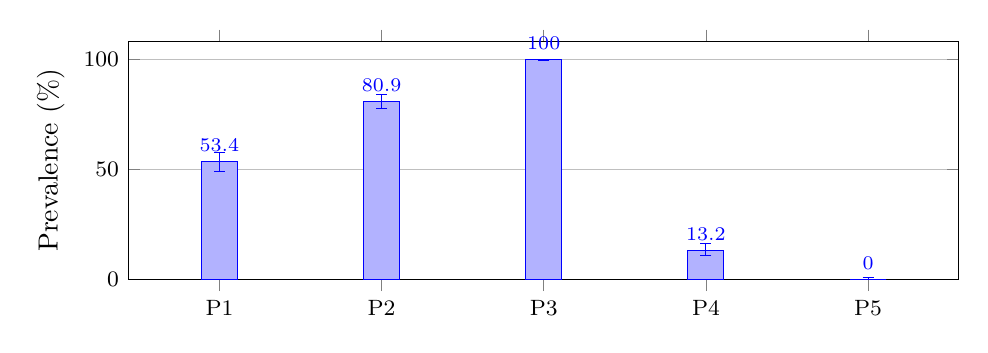
\begin{tikzpicture}
\begin{axis}[
  ybar, bar width=13pt,
  width=\linewidth, height=4.6cm,
  ymin=0, ymax=108, ylabel={Prevalence (\%)},
  symbolic x coords={P1,P2,P3,P4,P5},
  xtick=data, enlarge x limits=0.14,
  nodes near coords, nodes near coords align={vertical},
  every node near coord/.append style={font=\scriptsize},
  ymajorgrids, tick label style={font=\footnotesize},
]
% asymmetric explicit errors:  += (0, upper)  -= (0, lower)
\addplot+[error bars/.cd, y dir=both, y explicit]
coordinates {
  (P1,53.4)  += (0,4.2)  -= (0,4.3)
  (P2,80.9)  += (0,3.2)  -= (0,3.5)
  (P3,100.0) += (0,0.0)  -= (0,0.7)
  (P4,13.2)  += (0,3.2)  -= (0,2.6)
  (P5,0.0)   += (0,0.7)  -= (0,0.0)
};
\end{axis}
\end{tikzpicture}
\caption{Prevalence of cited verification weaknesses across 530 distinct
JWT-validating configurations, with Wilson 95\% confidence intervals.
P1 unbound audience; P2 no required claims; P3 no algorithm pinning \emph{in
configuration} (library-default caveat, \S\ref{sec:results}); P4 multi-issuer
(descriptive); P5 clock skew $>5$\,min (now read from Envoy
\texttt{clock\_skew\_seconds}; the widest observed is 60\,s). An independently
validated extractor; a hand-labelled gold standard is still pending
(\S\ref{sec:limitations}).}
\label{fig:prevalence}
\end{figure}

\noindent\textbf{Drift (RQ: how contracts change over time).}
Longitudinal analysis over commit history is future work. Today we validate the
drift \emph{classifier} on a 1{,}226-pair synthetic corpus at 100\% recall / 0\%
FPR, with mutation testing (24 mutants, 100\% killed) and a held-out adversarial
set at Youden 0.75. \gate{Drift in the wild, over real commit histories, is left to
the full study.}

\section{Limitations and threats to validity}\label{sec:limitations}
\textbf{Declared, not effective.} We measure the contract configuration declares,
not what the running verifier enforces. A configured check can still be skipped by
buggy verifier code, and a check absent from configuration can still hold because a
library default supplies it; conversely an implementation flaw (accepting
\texttt{alg=none}, RS/HS confusion) is invisible to us. We therefore report an
absent check as ``not set in configuration,'' not as a confirmed vulnerability, and
closing this gap needs live probing or a library-defaults database, which we leave
to future work. \textbf{Profile dependence.} Which checks are mandatory depends on
the token profile: audience and issuer validation are required for RFC~9068 access
tokens but optional for a bare RFC~7519 JWT, so an ``unbound audience'' is a
weakness only under a profile that requires binding; we measure the configured check
and name the profile where the corpus reveals it. \textbf{Templating:} $\approx$13\% of corpus files are
Helm-templated and $\approx$8\% carry kustomize/variable markers, so roughly one in
five configurations is under-resolved without rendering. \textbf{Selection bias:}
public configuration skews to samples, demos, and OSS and is not representative of
private enterprise deployments; this must be stated, not hidden. \textbf{Proxy
oracles:} \S\ref{sec:validation}'s recall/precision are automated approximations
pending human labels. \textbf{Ethics:} we use only public configuration, read
only; we do not probe third-party live endpoints and handle no real tokens;
identifiable high-severity findings follow responsible disclosure.

\section{Related work}\label{sec:related}
\noindent\textbf{In-the-wild web-authentication and SSO measurement.} The closest
line of work measures deployed authentication. Early studies inspect a small set of
sites by hand and show that SSO and OAuth failures are driven by deployment and
implementation choices rather than protocol flaws~\cite{authzmeas2012wangsignmein,authzmeas2012sunoauth}.
Later work makes this a population measurement: SSOScan automatically tests a fixed
catalog of five SSO vulnerabilities across the top 20{,}000 sites and finds that over
20\% of Facebook-SSO sites carry a serious flaw~\cite{authzmeas2014ssoscan}, and
subsequent studies measure sign-off and session handling, dual-window SSO, and SSO
adoption across the Tranco list~\cite{authzmeas2018singlesignoff,authzmeas2022distinct,authzmeas2023ssomonitor};
the OpenID Connect attack classes are systematized by Mainka et al.~\cite{authzmeas2017soksso}.
SSOScan is our closest methodological ancestor: automated detection of a fixed
weakness catalog over a crawled population. We keep that ambition but change the
object and the vantage point. We read the declared verification contract out of
static mesh and proxy configuration rather than driving a runtime login flow, which
reaches services no crawler can log into and separates what a service declares from
what it enforces.

\noindent\textbf{Large-scale misconfiguration measurement.} Our methodology follows
a well-established template: crawl a population, report the prevalence of a concrete
weakness, and quantify uncertainty. Studies of the HTTPS certificate ecosystem and
of Heartbleed turn repeated scans into a structured prevalence
picture~\cite{authzmeas2013httpsecosystem,authzmeas2014heartbleed}; the email-delivery
study measures adoption of \emph{declared} security policies (SPF, DKIM, DMARC)
across more than 700{,}000 servers~\cite{authzmeas2015emaildelivery}; and studies of
HTTPS adoption, Content Security Policy, CORS, and S3 buckets measure how a declared
per-service policy is set or fails at scale~\cite{authzmeas2017httpsadoption,authzmeas2016csp,authzmeas2018cors,authzmeas2018s3buckets}.
We adopt this template, including confidence intervals and a replication-style
validation of recall and precision, and apply it to a surface none of these touch,
the JWT authorization contract.

\noindent\textbf{IaC and configuration security.} Repository-mining studies quantify
security weaknesses in declarative infrastructure code: the Seven Sins study derives
smells from 1{,}726 scripts and counts occurrences across hundreds of
repositories~\cite{authzmeas2019sevensins}, replicated at larger scale and across
technologies~\cite{authzmeas2021iacreplication,authzmeas2022glitch}, and Kubernetes
security practice is systematized separately~\cite{authzmeas2020k8scommandments}.
Practitioner scanners (Checkov, KICS, Terrascan, Semgrep) and policy-as-code
engines~\cite{authzmeas2024checkov,authzmeas2024kics,authzmeas2024terrascan,authzmeas2024semgrep,authzmeas2024opa}
apply rule sets to individual files. These target generic hygiene (hard-coded
secrets, weak crypto) and check rules per file; we instead normalize heterogeneous
mesh and proxy configuration into one typed authorization contract per service and
measure its properties, and our negative control targets the attribution errors that
per-file pattern-matching is prone to.

\noindent\textbf{Formal analysis and config-as-contract.} A body of formal and
attack analysis establishes \emph{which} issuer, audience, algorithm, and endpoint
behaviours are load-bearing, for SAML, OAuth, and OpenID
Connect~\cite{authzmeas2008samlsso,authzmeas2012websanalysis,authzmeas2016oauthformal,authzmeas2017oidcformal};
the concrete JWT weaknesses we count (\texttt{alg=none}, RS/HS key confusion) are
documented by practitioners~\cite{authzmeas2015jwtlibs,authzmeas2024portswiggerjwt}
and codified in RFC~8725~\cite{rfc8725}. We cite these for the properties and then
measure how often deployments violate them rather than re-arguing relevance. The
idea of deriving a policy model from static configuration has a precedent in Batfish,
which parses heterogeneous device configuration into a vendor-independent model and
checks properties over it~\cite{authzmeas2015batfish}, and in ABAC policy
mining~\cite{authzmeas2015abacmining}; consumer-driven contract testing (Pact) shares
the ``contract'' framing~\cite{authzmeas2024pact}. None recovers a JWT authorization
contract or measures one across a population.

\noindent\textbf{Agent and MCP authorization.} Indirect prompt injection makes
token-scoped, verifiable authorization necessary for autonomous
agents~\cite{authzmeas2023promptinjection}, and recent measurements of live remote
MCP servers report widespread missing authentication and OAuth
flaws~\cite{authzmeas2026mcpauthmeas,authzmeas2026mcpexposed}. These show the same
population-measurement method reaching the agent frontier, where the declared-versus-effective
contract framing of this paper is the natural lens to carry forward.

\section{Future work}\label{sec:future}
Three extensions follow directly. (i) Pairing the static reading with live probing
would close the declared-vs-effective gap this paper is careful to leave open,
turning ``not set in configuration'' into a confirmed runtime behaviour. (ii) The
content-addressed contract makes \emph{drift} measurable over commit history: do
contracts widen more than they narrow, and are widenings tied to reviewable events?
(iii) The same instrument extends to the agent and MCP frontier, where OAuth/MCP
tokens carry the same issuer, audience, and claim checks on a faster-moving surface.

\section{Conclusion}
A service's decision to accept a token is configuration, declared across meshes,
proxies, and identity providers and rarely collected in one place. We make that
declared authorization contract an object that can be derived, measured, versioned,
and validated, we separate it from the effective enforcement that configuration
cannot show, and we measure it across 2{,}718 repositories with a methodology
honest about its own limits. The instrument and corpus are released so the
measurement is reproducible and extensible.

\section*{Ethics considerations}\label{sec:ethics}
This study measures only \emph{public} configuration, fetched read-only at pinned
commits, and never probes third-party live endpoints or handles real tokens; the
attack surface it characterises is exercised only against local, self-owned
negative-control fixtures. We report \emph{population} prevalence, never a verdict
on any single project, and we name no project as insecure. For any identifiable,
high-severity finding tied to a specific owner we follow coordinated responsible
disclosure before publication, allowing reasonable remediation time. The corpus
respects source licences (recorded per artifact) and robots/rate-limit norms of the
hosting platform. We see no human-subjects concerns; no personal data is collected.

\section*{Open science}\label{sec:openscience}
In keeping with open-science expectations, we release the discovery instrument, the
measurement harness (prevalence with Wilson CIs), the kind-aware validator, the
non-circular negative-control precision test, the analysis scripts, and the corpus
\emph{manifest} (repository + commit SHA + licence per artifact) so the measurement
is reproducible from public sources. \gate{At camera-ready we will add a DOI-pinned
archival snapshot and, where the venue offers it, Artifact-Evaluation ``Available'' and
``Reproduced'' badges.}

\section*{Artifact availability}\label{sec:artifact}
The instrument, harness, validator, negative-control test, and corpus manifest are
open source under the MIT licence. \gate{The archival DOI will be added at
camera-ready.}
 to bring
% back the loud [PENDING]/[NOTE] markers for internal tracking.
\ifdefined\ifsubmission\else\expandafter\newif\csname ifsubmission\endcsname\submissiontrue\fi
% \gate{...}: forward-looking text. Submission -> plain prose; draft -> [PENDING].
% Content is written to read as a finished future-work sentence either way.
\providecommand{\gate}[1]{\ifsubmission #1\else \textbf{[PENDING: #1]}\fi}
% \draftonly{...}: internal note. Submission -> nothing; draft -> [NOTE].
\providecommand{\draftonly}[1]{\ifsubmission\else \textbf{[NOTE: #1]}\fi}
% Let TeX relax line breaking on paragraphs with long unbreakable \texttt{} kind
% names (RequestAuthentication, AuthorizationPolicy) instead of overrunning the
% margin. Class-agnostic; applies under every venue wrapper.
\emergencystretch=3em

% The abstract lives in common/abstract.tex. acmart requires it BEFORE \maketitle,
% llncs/IEEEtran after, so an acmart wrapper \inputs it itself (and defines
% \keywayabstractdone); every other wrapper lets the body emit it here.
\ifdefined\keywayabstractdone\else\begin{abstract}
Whether a service accepts a JSON Web Token (JWT) is decided by configuration rather
than by application code: which token issuers it trusts, which audience a token must
name, which signing algorithms it accepts, and which claims it requires. In modern
deployments these settings are spread across a service mesh (e.g.\ Istio), an edge
proxy (e.g.\ Envoy), and an identity provider; they are rarely collected in one
place; and they change often, so a rotated signing key or a widened audience can
silently begin refusing valid requests or admitting tokens that should be rejected.
We call the resulting set of checks a service's implicit \emph{authorization
contract}. This paper makes that contract an object that can be \emph{derived} from
deployment configuration, measured, and compared across versions, and it separates
the \emph{declared} contract we extract from the \emph{effective} enforcement that
additionally depends on verifier code, library defaults, and software versions.

We derive authorization contracts from 2{,}718 public repositories and measure them
over 530 distinct JWT-validating configurations. None pins a signing algorithm in
configuration (each relies on a library default), 80.9\% require no claim beyond
issuer and audience, and 53.4\% leave the audience unbound; we report every figure
with a 95\% confidence interval. Because a measurement is only as sound as its
extractor, we validate discovery three ways and state the limit of each: recall
against an independent parse of the same configuration (issuers 96.0\%, audiences
98.2\%), precision against planted distractor values a correct extractor must
ignore, and a held-out split, labelled by an independent model that never sees the
extractor's output, that finds no over-attribution. We release the tool, the corpus
manifest, and the analysis.
\end{abstract}
\fi

\section{Introduction}
An engineer rotates a signing key on a Friday. No code changes; every test passes.
By Monday a downstream service is rejecting every valid user, because its verifier
cached the retired key longer than anyone realised. The same week, elsewhere, a
verifier quietly begins accepting a second audience nobody intended. Neither
failure lives in the code, and neither would be caught by reading it: both live in
the \emph{configuration} that actually decides whether a bearer token is accepted.

That configuration is an implicit specification: the issuers a verifier trusts,
the audiences it binds to, the algorithms it allows, the claims it requires, and
the JWKS behaviour of the library beneath it. We call it the \emph{authorization
contract}. It is spread across service meshes, proxies, identity providers, and
library defaults, it is almost never centralised, and it \emph{drifts}: a rotated
key, a widened audience, or a dropped claim turns valid users away (an outage) or
admits tokens that should be refused (a silent regression). As autonomous agents
begin carrying OAuth/MCP tokens on a user's behalf, the same contract now governs a
faster-moving, higher-stakes surface.

A caveat shapes the whole paper. What configuration states is the \emph{declared}
contract; whether a request is ultimately accepted is the \emph{effective}
behaviour, which also depends on the verifier's code, its library's defaults, and
its software version. A verifier may, for example, accept the \texttt{none}
algorithm because of an implementation flaw even where configuration says nothing,
and that is not visible in configuration at all. We measure the declared contract,
we say so throughout, and \S\ref{sec:background} and \S\ref{sec:limitations} make
the boundary between declared and effective explicit; where a declared value is
absent we distinguish ``not set in configuration'' from ``not enforced.''

This declared contract is where much of auth correctness is decided, and yet almost
nobody measures it at scale. Two kinds of tooling exist and neither answers ``what
do deployed authorization contracts look like across a population, and how healthy
are they?'' Static code scanners reason about source, not about which configured
verifier trusts which issuer; gateways and identity providers are the thing being
configured, so they do not tell an operator whether that configuration is healthy.

\noindent\textbf{Contributions.}
(i) We define the \emph{authorization contract} and give a method that derives it
from heterogeneous deployment configuration (Istio, Envoy, OIDC) with per-field
provenance and content-addressed versioning, separating the declared contract from
effective enforcement (\S\ref{sec:method}).
(ii) We measure how common concrete, normatively grounded weaknesses are across
2{,}718 public repositories and 530 JWT-validating configurations, with confidence
intervals and a co-occurrence analysis (\S\ref{sec:results}).
(iii) We give a validation methodology that is explicit about its own limits:
recall against an independent parse, a non-circular negative control for precision,
and a held-out over-attribution split, each with its failure mode stated
(\S\ref{sec:validation}).
(iv) We release the instrument, the corpus manifest, and the analysis so the study
is reproducible from public sources (\S\ref{sec:artifact}).

\section{Background}\label{sec:background}

\noindent\textbf{JWT verification.} A JSON Web Token is a signed statement of
claims: a header naming the signing algorithm, a payload of claims (including
\texttt{iss}, the issuer; \texttt{aud}, the intended audience; \texttt{exp}, the
expiry), and a signature. To accept a token, a verifier must (1) fetch the issuer's
public keys, in practice from a JSON Web Key Set (JWKS) endpoint, and verify the
signature; (2) check that \texttt{iss} is a trusted issuer; (3) check that
\texttt{aud} names this resource; (4) accept only an allow-list of signing
algorithms; and (5) enforce any additional required claims (roles, scopes, tenant).
Each step has a normative source. RFC~8725 (JSON Web Token Best Current Practices)
requires an explicit algorithm allow-list (\S3.1) and validation of all security
claims (\S3.9); RFC~9068 profiles JWT \emph{access tokens} and makes audience and
issuer validation mandatory for that profile; RFC~8707 (resource indicators) and
RFC~9728 (protected-resource metadata) bind a token to the resource it was minted
for. Which checks are mandatory therefore depends partly on the token profile in
use, a point we return to in \S\ref{sec:limitations}.

\noindent\textbf{Where the contract lives.} Few services implement these checks in
application code. In a service mesh the checks are declared as configuration and
enforced by a sidecar or gateway. Under Istio, a \texttt{RequestAuthentication}
resource declares the issuer, the JWKS source, and the accepted audiences, while an
\texttt{AuthorizationPolicy} declares required claims as \texttt{when} conditions on
\texttt{request.auth.claims[...]}; under Envoy, a \texttt{jwt\_authn} filter carries
the providers, audiences, and clock-skew tolerance. These resources usually live in
\emph{different files}, and the effective contract for one workload is their union.
Figure~\ref{fig:example} shows a minimal pair.

\begin{figure}[t]
\footnotesize
\begin{verbatim}
kind: RequestAuthentication      # issuer + audience
spec:
  selector: {matchLabels: {app: orders}}
  jwtRules:
  - issuer: "https://idp.example/realms/main"
    jwksUri: "https://idp.example/jwks.json"
    audiences: ["orders-api"]
---
kind: AuthorizationPolicy        # a required claim
spec:
  selector: {matchLabels: {app: orders}}
  rules:
  - when:
    - key: request.auth.claims[groups]
      values: ["ops"]
\end{verbatim}
\caption{The declared authorization contract for the \texttt{orders} workload,
spread across two resources: trust \texttt{idp.example}, require audience
\texttt{orders-api}, and require a \texttt{groups} claim of \texttt{ops}. No signing
algorithm is pinned, so the mesh applies its library default (\S\ref{sec:results}).}
\label{fig:example}
\end{figure}

\noindent\textbf{Declared vs.\ effective; terminology.} We measure the
\emph{declared} contract in resources like these. The \emph{effective} behaviour
can differ: a verifier might skip a check, honour a dangerous default, or carry an
implementation bug (accepting \texttt{alg=none}, confusing RS256 and HS256). Those
are code, not configuration, and outside the reach of a static reading; we flag the
absence of a configured check as ``not set in configuration,'' never as a confirmed
runtime vulnerability. We use \emph{consumer} for the verifying entity a contract
belongs to (an Istio workload, an Envoy route), and we restrict \emph{authorization
contract} to \emph{token validation} (is this token acceptable?), as distinct from
resource-level authorization (may this subject perform this action?), which is a
separate layer we do not measure.

\section{Deriving authorization contracts}\label{sec:method}
We derive one contract per \emph{consumer} (\S\ref{sec:background}) from the
configuration that governs it. Source-specific \emph{discoverers} parse each format
(Istio \texttt{RequestAuthentication} and \texttt{AuthorizationPolicy}, Envoy
\texttt{jwt\_authn}, and OIDC/Keycloak registries) into a common contract of
issuers, audiences, algorithms, required claims, and JWKS behaviour.

Deriving a contract is not a one-resource read, because the checks are split across
resources (\S\ref{sec:background}). For the pair in Figure~\ref{fig:example}, the
\texttt{RequestAuthentication} contributes the issuer, JWKS source, and audience,
and the \texttt{AuthorizationPolicy} contributes the required \texttt{groups} claim;
we join them by the workload they select (\texttt{app: orders}) into a single
consumer whose contract carries all three. Attribution follows the mesh's own
semantics: a selector-less policy applies to every workload in its namespace, and
in a namespace with a single JWT consumer a per-service claim policy attaches to
that consumer (the common edge-gateway pattern). The same join resolves audiences
declared in an \texttt{AuthorizationPolicy} condition on
\texttt{request.auth.audiences} rather than in the \texttt{RequestAuthentication}.

Every extracted field records \emph{provenance}: the source kind, the file
locator, and a confidence. Each measurement is therefore attributable to a line of
configuration and a human can check it (we use this in \S\ref{sec:validation}).
A library-defaults database records what a verifier does when configuration is
silent, kept separate from what configuration states so the two are never conflated.
Consumers are assembled into a content-addressed \texttt{ContractVersion}, which
makes change detection exact equality and lets us diff one deployment's contract
against another or against its own history.

\section{Corpus construction}\label{sec:corpus}
We crawl public GitHub read-only for real auth configuration (Istio
\texttt{RequestAuthentication}, Envoy \texttt{jwt\_authn}, Istio claim conditions),
recording repository, blob SHA, and licence for every artifact for reproducibility
and attribution. We fetch public repositories only, cap files per repository to
limit monorepo dominance, and analyse \emph{per repository} so a
\texttt{RequestAuthentication} and its \texttt{AuthorizationPolicy} (usually in
separate files) are resolved together while distinct repositories remain isolated.
Two cleaning steps address representativeness: we exclude tutorial/vendored copies
by path (matched against the full locator, so \texttt{testdata/}, \texttt{vendor/},
and \texttt{/e2e/} components are caught, not only basenames), and we deduplicate
identical configurations (a canonical sample pasted across repositories counts
once). The corpus is 5{,}214 files across 2{,}718 public repositories, yielding 778
JWT-validating configurations, or 530 after deduplication. \gate{A full study will
push the corpus further toward $10^4$ services, add OIDC/MCP sources, and report a
selection-bias analysis against the public-configuration population.}

\section{Validation methodology}\label{sec:validation}
Measurement is only as good as the extractor. We validate discovery three ways, for
recall, for precision, and for over-attribution, and are explicit about what each
can and cannot establish.

\noindent\textbf{Recall (kind-aware independent parse).} An independent YAML parse
of each repository yields the declared issuers/audiences/claims; we compare to what
discovery captured, per repository. The independent parser also
\emph{over-declares}: it scrapes \texttt{issuer:} keys and claim-like strings from
non-auth resources (a ConfigMap, an annotation). We therefore measure recall only
against values in \emph{genuine} auth resources (RequestAuthentication /
AuthorizationPolicy / Envoy JWT). Adjudicated recall is issuers 96.0\%, audiences
98.2\%, and claims 86.0\% (scoped to repositories where a JWT consumer exists;
claims declared in repositories whose RequestAuthentication is absent from the
corpus have no consumer to attach to). The adjudication removed 106 parser
over-declarations (65 issuers, 27 audiences, 14 claims), which both raises the
honest recall and demonstrates the proxy oracle is itself imperfect. The issuer
figure rose from an earlier 89.6\% once a document-splitting bug was fixed: a single
templated or malformed YAML document had been aborting the rest of its file, so the
earlier recall was depressed by the extractor, not by the corpus.

\noindent\textbf{Precision (non-circular negative control).} An independent-parse
oracle cannot honestly measure precision: it reads the same fields as the
extractor, so captures are almost always a subset and precision $\approx 100\%$
\emph{by construction}. We therefore use a negative control: configurations with
planted distractor values a correct discoverer must ignore: a commented-out
issuer, an \texttt{issuer:}/claim in a non-auth ConfigMap, a claim behind a
non-matching AuthorizationPolicy selector (the real attribution risk), and strings
in annotations. Result: 4 planted, 0 leaked, with real values still captured.

\noindent\textbf{Over-attribution (held-out split).} To measure how often discovery
\emph{adds} a value that is not really there, we take every captured/declared
disagreement, label each with an independent model that reads only the raw
configuration and never the extractor's output (so the grading is non-circular),
and split the labelled set 70/30 by repository so no repository informs both sides.
On the held-out test split, precision is 100\% and over-attribution is 0.0\% (0 of 6
captured-only values are spurious or mis-attributed); on the full labelled set,
precision 100\% and over-attribution 0.0\%. This split is what caught, and then
confirmed the fix for, an Envoy test-fixture leak and a claim mis-attribution during
development.

\noindent\textbf{Gold standard.} All three above are automated or model-assisted
proxies. For a population-level ground truth we draw a stratified random sample of
401 \mbox{(repo, field, value)} rows across the corpus, powered for a $\pm$1.8\%
precision and $\pm$2.4\% recall confidence interval, and have each adjudicated by
hand as real, correctly attributed, or spurious; a model drafts a first-pass label
that the human confirms or corrects, and a blind subset gives an un-anchored
inter-annotator agreement (Cohen's $\kappa$). \gate{We report the hand-validated
precision, recall, and $\kappa$ in the final version; the automated results above
are what the gold standard refines.}

\section{Results}\label{sec:results}
We report prevalence over the 530 deduplicated JWT-validating configurations, each
with a 95\% Wilson confidence interval (the Wilson interval is preferred over the
normal approximation for proportions near 0 or 1). These figures come from the
independently validated extractor of \S\ref{sec:validation}; the hand-validated
gold standard refines the \emph{validation} numbers, not the prevalence below.

\noindent\textbf{Prevalence.} Over 530 distinct JWT-validating configurations
(Wilson 95\% CIs): no algorithm pinning \emph{in configuration} 100\%
[99.3, 100]; no required claims 80.9\% [77.4, 84.1]; unbound audience 53.4\%
[49.1, 57.6]; multi-issuer trust 13.2\% [10.6, 16.4] (descriptive, not a weakness);
clock skew $>5$\,min 0.0\% [0.0, 0.7]. The algorithm-pinning figure reflects
reliance on the verifying \emph{library's default}, which configuration does not
restate. This is a static-vs-runtime gap, not a 100\% vulnerability rate; we report
it as ``not pinned in config.'' The clock-skew figure is now read directly from
Envoy \texttt{clock\_skew\_seconds} rather than assumed: of the configurations that
set it the widest is 60\,s, so the 0.0\% above the 5-minute threshold is measured,
not merely unobserved. The earlier draft's 42.2\% unbound-audience figure, over a
102-configuration pilot, rises to 53.4\% on this larger and more representative
corpus; the direction and the majority finding are unchanged.

\noindent\textbf{Co-occurrence.} Weaknesses travel together. No-required-claims and
no-algorithm-pinning co-occur in 80.9\% of configurations; unbound-audience with
no-algorithm-pinning in 53.4\%; unbound-audience with no-required-claims in 43.8\%
(lift $\approx$1.0, i.e. roughly independent rather than mutually reinforcing).

\noindent\textbf{Static/runtime frontier.} Four of the five check types are
conclusive from configuration alone; only algorithm pinning carries the
library-default caveat. Of 1{,}312 weakness flags raised, 782 (60\%) are
static-conclusive and 530 carry that caveat, quantifying how much of the contract a
purely static reading can settle.

% Prevalence figure (n=530 distinct JWT-validating configs, scaled corpus).
% Real values with Wilson 95% CIs (asymmetric). Requires pgfplots in the preamble
% (the wrappers add it). \input this inside the Results section.
\begin{figure}[t]
\centering
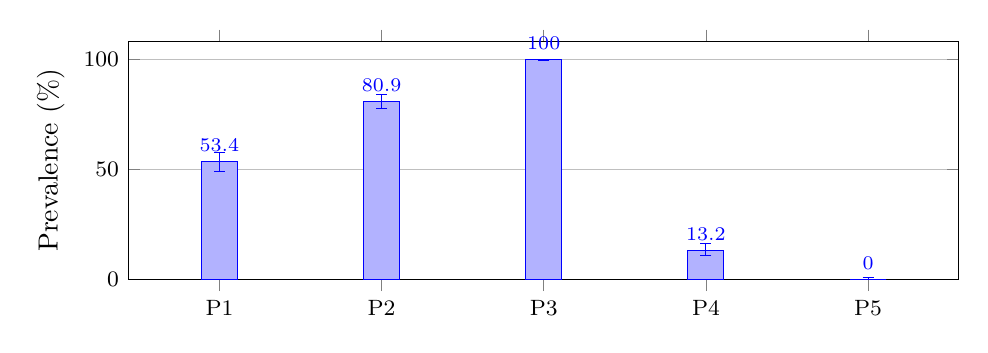
\begin{tikzpicture}
\begin{axis}[
  ybar, bar width=13pt,
  width=\linewidth, height=4.6cm,
  ymin=0, ymax=108, ylabel={Prevalence (\%)},
  symbolic x coords={P1,P2,P3,P4,P5},
  xtick=data, enlarge x limits=0.14,
  nodes near coords, nodes near coords align={vertical},
  every node near coord/.append style={font=\scriptsize},
  ymajorgrids, tick label style={font=\footnotesize},
]
% asymmetric explicit errors:  += (0, upper)  -= (0, lower)
\addplot+[error bars/.cd, y dir=both, y explicit]
coordinates {
  (P1,53.4)  += (0,4.2)  -= (0,4.3)
  (P2,80.9)  += (0,3.2)  -= (0,3.5)
  (P3,100.0) += (0,0.0)  -= (0,0.7)
  (P4,13.2)  += (0,3.2)  -= (0,2.6)
  (P5,0.0)   += (0,0.7)  -= (0,0.0)
};
\end{axis}
\end{tikzpicture}
\caption{Prevalence of cited verification weaknesses across 530 distinct
JWT-validating configurations, with Wilson 95\% confidence intervals.
P1 unbound audience; P2 no required claims; P3 no algorithm pinning \emph{in
configuration} (library-default caveat, \S\ref{sec:results}); P4 multi-issuer
(descriptive); P5 clock skew $>5$\,min (now read from Envoy
\texttt{clock\_skew\_seconds}; the widest observed is 60\,s). An independently
validated extractor; a hand-labelled gold standard is still pending
(\S\ref{sec:limitations}).}
\label{fig:prevalence}
\end{figure}

\noindent\textbf{Drift (RQ: how contracts change over time).}
Longitudinal analysis over commit history is future work. Today we validate the
drift \emph{classifier} on a 1{,}226-pair synthetic corpus at 100\% recall / 0\%
FPR, with mutation testing (24 mutants, 100\% killed) and a held-out adversarial
set at Youden 0.75. \gate{Drift in the wild, over real commit histories, is left to
the full study.}

\section{Limitations and threats to validity}\label{sec:limitations}
\textbf{Declared, not effective.} We measure the contract configuration declares,
not what the running verifier enforces. A configured check can still be skipped by
buggy verifier code, and a check absent from configuration can still hold because a
library default supplies it; conversely an implementation flaw (accepting
\texttt{alg=none}, RS/HS confusion) is invisible to us. We therefore report an
absent check as ``not set in configuration,'' not as a confirmed vulnerability, and
closing this gap needs live probing or a library-defaults database, which we leave
to future work. \textbf{Profile dependence.} Which checks are mandatory depends on
the token profile: audience and issuer validation are required for RFC~9068 access
tokens but optional for a bare RFC~7519 JWT, so an ``unbound audience'' is a
weakness only under a profile that requires binding; we measure the configured check
and name the profile where the corpus reveals it. \textbf{Templating:} $\approx$13\% of corpus files are
Helm-templated and $\approx$8\% carry kustomize/variable markers, so roughly one in
five configurations is under-resolved without rendering. \textbf{Selection bias:}
public configuration skews to samples, demos, and OSS and is not representative of
private enterprise deployments; this must be stated, not hidden. \textbf{Proxy
oracles:} \S\ref{sec:validation}'s recall/precision are automated approximations
pending human labels. \textbf{Ethics:} we use only public configuration, read
only; we do not probe third-party live endpoints and handle no real tokens;
identifiable high-severity findings follow responsible disclosure.

\section{Related work}\label{sec:related}
\noindent\textbf{In-the-wild web-authentication and SSO measurement.} The closest
line of work measures deployed authentication. Early studies inspect a small set of
sites by hand and show that SSO and OAuth failures are driven by deployment and
implementation choices rather than protocol flaws~\cite{authzmeas2012wangsignmein,authzmeas2012sunoauth}.
Later work makes this a population measurement: SSOScan automatically tests a fixed
catalog of five SSO vulnerabilities across the top 20{,}000 sites and finds that over
20\% of Facebook-SSO sites carry a serious flaw~\cite{authzmeas2014ssoscan}, and
subsequent studies measure sign-off and session handling, dual-window SSO, and SSO
adoption across the Tranco list~\cite{authzmeas2018singlesignoff,authzmeas2022distinct,authzmeas2023ssomonitor};
the OpenID Connect attack classes are systematized by Mainka et al.~\cite{authzmeas2017soksso}.
SSOScan is our closest methodological ancestor: automated detection of a fixed
weakness catalog over a crawled population. We keep that ambition but change the
object and the vantage point. We read the declared verification contract out of
static mesh and proxy configuration rather than driving a runtime login flow, which
reaches services no crawler can log into and separates what a service declares from
what it enforces.

\noindent\textbf{Large-scale misconfiguration measurement.} Our methodology follows
a well-established template: crawl a population, report the prevalence of a concrete
weakness, and quantify uncertainty. Studies of the HTTPS certificate ecosystem and
of Heartbleed turn repeated scans into a structured prevalence
picture~\cite{authzmeas2013httpsecosystem,authzmeas2014heartbleed}; the email-delivery
study measures adoption of \emph{declared} security policies (SPF, DKIM, DMARC)
across more than 700{,}000 servers~\cite{authzmeas2015emaildelivery}; and studies of
HTTPS adoption, Content Security Policy, CORS, and S3 buckets measure how a declared
per-service policy is set or fails at scale~\cite{authzmeas2017httpsadoption,authzmeas2016csp,authzmeas2018cors,authzmeas2018s3buckets}.
We adopt this template, including confidence intervals and a replication-style
validation of recall and precision, and apply it to a surface none of these touch,
the JWT authorization contract.

\noindent\textbf{IaC and configuration security.} Repository-mining studies quantify
security weaknesses in declarative infrastructure code: the Seven Sins study derives
smells from 1{,}726 scripts and counts occurrences across hundreds of
repositories~\cite{authzmeas2019sevensins}, replicated at larger scale and across
technologies~\cite{authzmeas2021iacreplication,authzmeas2022glitch}, and Kubernetes
security practice is systematized separately~\cite{authzmeas2020k8scommandments}.
Practitioner scanners (Checkov, KICS, Terrascan, Semgrep) and policy-as-code
engines~\cite{authzmeas2024checkov,authzmeas2024kics,authzmeas2024terrascan,authzmeas2024semgrep,authzmeas2024opa}
apply rule sets to individual files. These target generic hygiene (hard-coded
secrets, weak crypto) and check rules per file; we instead normalize heterogeneous
mesh and proxy configuration into one typed authorization contract per service and
measure its properties, and our negative control targets the attribution errors that
per-file pattern-matching is prone to.

\noindent\textbf{Formal analysis and config-as-contract.} A body of formal and
attack analysis establishes \emph{which} issuer, audience, algorithm, and endpoint
behaviours are load-bearing, for SAML, OAuth, and OpenID
Connect~\cite{authzmeas2008samlsso,authzmeas2012websanalysis,authzmeas2016oauthformal,authzmeas2017oidcformal};
the concrete JWT weaknesses we count (\texttt{alg=none}, RS/HS key confusion) are
documented by practitioners~\cite{authzmeas2015jwtlibs,authzmeas2024portswiggerjwt}
and codified in RFC~8725~\cite{rfc8725}. We cite these for the properties and then
measure how often deployments violate them rather than re-arguing relevance. The
idea of deriving a policy model from static configuration has a precedent in Batfish,
which parses heterogeneous device configuration into a vendor-independent model and
checks properties over it~\cite{authzmeas2015batfish}, and in ABAC policy
mining~\cite{authzmeas2015abacmining}; consumer-driven contract testing (Pact) shares
the ``contract'' framing~\cite{authzmeas2024pact}. None recovers a JWT authorization
contract or measures one across a population.

\noindent\textbf{Agent and MCP authorization.} Indirect prompt injection makes
token-scoped, verifiable authorization necessary for autonomous
agents~\cite{authzmeas2023promptinjection}, and recent measurements of live remote
MCP servers report widespread missing authentication and OAuth
flaws~\cite{authzmeas2026mcpauthmeas,authzmeas2026mcpexposed}. These show the same
population-measurement method reaching the agent frontier, where the declared-versus-effective
contract framing of this paper is the natural lens to carry forward.

\section{Future work}\label{sec:future}
Three extensions follow directly. (i) Pairing the static reading with live probing
would close the declared-vs-effective gap this paper is careful to leave open,
turning ``not set in configuration'' into a confirmed runtime behaviour. (ii) The
content-addressed contract makes \emph{drift} measurable over commit history: do
contracts widen more than they narrow, and are widenings tied to reviewable events?
(iii) The same instrument extends to the agent and MCP frontier, where OAuth/MCP
tokens carry the same issuer, audience, and claim checks on a faster-moving surface.

\section{Conclusion}
A service's decision to accept a token is configuration, declared across meshes,
proxies, and identity providers and rarely collected in one place. We make that
declared authorization contract an object that can be derived, measured, versioned,
and validated, we separate it from the effective enforcement that configuration
cannot show, and we measure it across 2{,}718 repositories with a methodology
honest about its own limits. The instrument and corpus are released so the
measurement is reproducible and extensible.

\section*{Ethics considerations}\label{sec:ethics}
This study measures only \emph{public} configuration, fetched read-only at pinned
commits, and never probes third-party live endpoints or handles real tokens; the
attack surface it characterises is exercised only against local, self-owned
negative-control fixtures. We report \emph{population} prevalence, never a verdict
on any single project, and we name no project as insecure. For any identifiable,
high-severity finding tied to a specific owner we follow coordinated responsible
disclosure before publication, allowing reasonable remediation time. The corpus
respects source licences (recorded per artifact) and robots/rate-limit norms of the
hosting platform. We see no human-subjects concerns; no personal data is collected.

\section*{Open science}\label{sec:openscience}
In keeping with open-science expectations, we release the discovery instrument, the
measurement harness (prevalence with Wilson CIs), the kind-aware validator, the
non-circular negative-control precision test, the analysis scripts, and the corpus
\emph{manifest} (repository + commit SHA + licence per artifact) so the measurement
is reproducible from public sources. \gate{At camera-ready we will add a DOI-pinned
archival snapshot and, where the venue offers it, Artifact-Evaluation ``Available'' and
``Reproduced'' badges.}

\section*{Artifact availability}\label{sec:artifact}
The instrument, harness, validator, negative-control test, and corpus manifest are
open source under the MIT licence. \gate{The archival DOI will be added at
camera-ready.}
. Every unfinished number is wrapped in \gate{...}.
% Submission vs. working-copy rendering. Default: submission (clean prose). A
% wrapper can predefine \submissionfalse before % Shared body for the Paper A measurement study. Class-agnostic: the per-venue
% main.tex sets \documentclass, title, authors, and \begin{document}, then
% % Shared body for the Paper A measurement study. Class-agnostic: the per-venue
% main.tex sets \documentclass, title, authors, and \begin{document}, then
% % Shared body for the Paper A measurement study. Class-agnostic: the per-venue
% main.tex sets \documentclass, title, authors, and \begin{document}, then
% \input{../common/body}. Every unfinished number is wrapped in \gate{...}.
% Submission vs. working-copy rendering. Default: submission (clean prose). A
% wrapper can predefine \submissionfalse before \input{../common/body} to bring
% back the loud [PENDING]/[NOTE] markers for internal tracking.
\ifdefined\ifsubmission\else\expandafter\newif\csname ifsubmission\endcsname\submissiontrue\fi
% \gate{...}: forward-looking text. Submission -> plain prose; draft -> [PENDING].
% Content is written to read as a finished future-work sentence either way.
\providecommand{\gate}[1]{\ifsubmission #1\else \textbf{[PENDING: #1]}\fi}
% \draftonly{...}: internal note. Submission -> nothing; draft -> [NOTE].
\providecommand{\draftonly}[1]{\ifsubmission\else \textbf{[NOTE: #1]}\fi}
% Let TeX relax line breaking on paragraphs with long unbreakable \texttt{} kind
% names (RequestAuthentication, AuthorizationPolicy) instead of overrunning the
% margin. Class-agnostic; applies under every venue wrapper.
\emergencystretch=3em

% The abstract lives in common/abstract.tex. acmart requires it BEFORE \maketitle,
% llncs/IEEEtran after, so an acmart wrapper \inputs it itself (and defines
% \keywayabstractdone); every other wrapper lets the body emit it here.
\ifdefined\keywayabstractdone\else\input{abstract}\fi

\section{Introduction}
An engineer rotates a signing key on a Friday. No code changes; every test passes.
By Monday a downstream service is rejecting every valid user, because its verifier
cached the retired key longer than anyone realised. The same week, elsewhere, a
verifier quietly begins accepting a second audience nobody intended. Neither
failure lives in the code, and neither would be caught by reading it: both live in
the \emph{configuration} that actually decides whether a bearer token is accepted.

That configuration is an implicit specification: the issuers a verifier trusts,
the audiences it binds to, the algorithms it allows, the claims it requires, and
the JWKS behaviour of the library beneath it. We call it the \emph{authorization
contract}. It is spread across service meshes, proxies, identity providers, and
library defaults, it is almost never centralised, and it \emph{drifts}: a rotated
key, a widened audience, or a dropped claim turns valid users away (an outage) or
admits tokens that should be refused (a silent regression). As autonomous agents
begin carrying OAuth/MCP tokens on a user's behalf, the same contract now governs a
faster-moving, higher-stakes surface.

A caveat shapes the whole paper. What configuration states is the \emph{declared}
contract; whether a request is ultimately accepted is the \emph{effective}
behaviour, which also depends on the verifier's code, its library's defaults, and
its software version. A verifier may, for example, accept the \texttt{none}
algorithm because of an implementation flaw even where configuration says nothing,
and that is not visible in configuration at all. We measure the declared contract,
we say so throughout, and \S\ref{sec:background} and \S\ref{sec:limitations} make
the boundary between declared and effective explicit; where a declared value is
absent we distinguish ``not set in configuration'' from ``not enforced.''

This declared contract is where much of auth correctness is decided, and yet almost
nobody measures it at scale. Two kinds of tooling exist and neither answers ``what
do deployed authorization contracts look like across a population, and how healthy
are they?'' Static code scanners reason about source, not about which configured
verifier trusts which issuer; gateways and identity providers are the thing being
configured, so they do not tell an operator whether that configuration is healthy.

\noindent\textbf{Contributions.}
(i) We define the \emph{authorization contract} and give a method that derives it
from heterogeneous deployment configuration (Istio, Envoy, OIDC) with per-field
provenance and content-addressed versioning, separating the declared contract from
effective enforcement (\S\ref{sec:method}).
(ii) We measure how common concrete, normatively grounded weaknesses are across
2{,}718 public repositories and 530 JWT-validating configurations, with confidence
intervals and a co-occurrence analysis (\S\ref{sec:results}).
(iii) We give a validation methodology that is explicit about its own limits:
recall against an independent parse, a non-circular negative control for precision,
and a held-out over-attribution split, each with its failure mode stated
(\S\ref{sec:validation}).
(iv) We release the instrument, the corpus manifest, and the analysis so the study
is reproducible from public sources (\S\ref{sec:artifact}).

\section{Background}\label{sec:background}

\noindent\textbf{JWT verification.} A JSON Web Token is a signed statement of
claims: a header naming the signing algorithm, a payload of claims (including
\texttt{iss}, the issuer; \texttt{aud}, the intended audience; \texttt{exp}, the
expiry), and a signature. To accept a token, a verifier must (1) fetch the issuer's
public keys, in practice from a JSON Web Key Set (JWKS) endpoint, and verify the
signature; (2) check that \texttt{iss} is a trusted issuer; (3) check that
\texttt{aud} names this resource; (4) accept only an allow-list of signing
algorithms; and (5) enforce any additional required claims (roles, scopes, tenant).
Each step has a normative source. RFC~8725 (JSON Web Token Best Current Practices)
requires an explicit algorithm allow-list (\S3.1) and validation of all security
claims (\S3.9); RFC~9068 profiles JWT \emph{access tokens} and makes audience and
issuer validation mandatory for that profile; RFC~8707 (resource indicators) and
RFC~9728 (protected-resource metadata) bind a token to the resource it was minted
for. Which checks are mandatory therefore depends partly on the token profile in
use, a point we return to in \S\ref{sec:limitations}.

\noindent\textbf{Where the contract lives.} Few services implement these checks in
application code. In a service mesh the checks are declared as configuration and
enforced by a sidecar or gateway. Under Istio, a \texttt{RequestAuthentication}
resource declares the issuer, the JWKS source, and the accepted audiences, while an
\texttt{AuthorizationPolicy} declares required claims as \texttt{when} conditions on
\texttt{request.auth.claims[...]}; under Envoy, a \texttt{jwt\_authn} filter carries
the providers, audiences, and clock-skew tolerance. These resources usually live in
\emph{different files}, and the effective contract for one workload is their union.
Figure~\ref{fig:example} shows a minimal pair.

\begin{figure}[t]
\footnotesize
\begin{verbatim}
kind: RequestAuthentication      # issuer + audience
spec:
  selector: {matchLabels: {app: orders}}
  jwtRules:
  - issuer: "https://idp.example/realms/main"
    jwksUri: "https://idp.example/jwks.json"
    audiences: ["orders-api"]
---
kind: AuthorizationPolicy        # a required claim
spec:
  selector: {matchLabels: {app: orders}}
  rules:
  - when:
    - key: request.auth.claims[groups]
      values: ["ops"]
\end{verbatim}
\caption{The declared authorization contract for the \texttt{orders} workload,
spread across two resources: trust \texttt{idp.example}, require audience
\texttt{orders-api}, and require a \texttt{groups} claim of \texttt{ops}. No signing
algorithm is pinned, so the mesh applies its library default (\S\ref{sec:results}).}
\label{fig:example}
\end{figure}

\noindent\textbf{Declared vs.\ effective; terminology.} We measure the
\emph{declared} contract in resources like these. The \emph{effective} behaviour
can differ: a verifier might skip a check, honour a dangerous default, or carry an
implementation bug (accepting \texttt{alg=none}, confusing RS256 and HS256). Those
are code, not configuration, and outside the reach of a static reading; we flag the
absence of a configured check as ``not set in configuration,'' never as a confirmed
runtime vulnerability. We use \emph{consumer} for the verifying entity a contract
belongs to (an Istio workload, an Envoy route), and we restrict \emph{authorization
contract} to \emph{token validation} (is this token acceptable?), as distinct from
resource-level authorization (may this subject perform this action?), which is a
separate layer we do not measure.

\section{Deriving authorization contracts}\label{sec:method}
We derive one contract per \emph{consumer} (\S\ref{sec:background}) from the
configuration that governs it. Source-specific \emph{discoverers} parse each format
(Istio \texttt{RequestAuthentication} and \texttt{AuthorizationPolicy}, Envoy
\texttt{jwt\_authn}, and OIDC/Keycloak registries) into a common contract of
issuers, audiences, algorithms, required claims, and JWKS behaviour.

Deriving a contract is not a one-resource read, because the checks are split across
resources (\S\ref{sec:background}). For the pair in Figure~\ref{fig:example}, the
\texttt{RequestAuthentication} contributes the issuer, JWKS source, and audience,
and the \texttt{AuthorizationPolicy} contributes the required \texttt{groups} claim;
we join them by the workload they select (\texttt{app: orders}) into a single
consumer whose contract carries all three. Attribution follows the mesh's own
semantics: a selector-less policy applies to every workload in its namespace, and
in a namespace with a single JWT consumer a per-service claim policy attaches to
that consumer (the common edge-gateway pattern). The same join resolves audiences
declared in an \texttt{AuthorizationPolicy} condition on
\texttt{request.auth.audiences} rather than in the \texttt{RequestAuthentication}.

Every extracted field records \emph{provenance}: the source kind, the file
locator, and a confidence. Each measurement is therefore attributable to a line of
configuration and a human can check it (we use this in \S\ref{sec:validation}).
A library-defaults database records what a verifier does when configuration is
silent, kept separate from what configuration states so the two are never conflated.
Consumers are assembled into a content-addressed \texttt{ContractVersion}, which
makes change detection exact equality and lets us diff one deployment's contract
against another or against its own history.

\section{Corpus construction}\label{sec:corpus}
We crawl public GitHub read-only for real auth configuration (Istio
\texttt{RequestAuthentication}, Envoy \texttt{jwt\_authn}, Istio claim conditions),
recording repository, blob SHA, and licence for every artifact for reproducibility
and attribution. We fetch public repositories only, cap files per repository to
limit monorepo dominance, and analyse \emph{per repository} so a
\texttt{RequestAuthentication} and its \texttt{AuthorizationPolicy} (usually in
separate files) are resolved together while distinct repositories remain isolated.
Two cleaning steps address representativeness: we exclude tutorial/vendored copies
by path (matched against the full locator, so \texttt{testdata/}, \texttt{vendor/},
and \texttt{/e2e/} components are caught, not only basenames), and we deduplicate
identical configurations (a canonical sample pasted across repositories counts
once). The corpus is 5{,}214 files across 2{,}718 public repositories, yielding 778
JWT-validating configurations, or 530 after deduplication. \gate{A full study will
push the corpus further toward $10^4$ services, add OIDC/MCP sources, and report a
selection-bias analysis against the public-configuration population.}

\section{Validation methodology}\label{sec:validation}
Measurement is only as good as the extractor. We validate discovery three ways, for
recall, for precision, and for over-attribution, and are explicit about what each
can and cannot establish.

\noindent\textbf{Recall (kind-aware independent parse).} An independent YAML parse
of each repository yields the declared issuers/audiences/claims; we compare to what
discovery captured, per repository. The independent parser also
\emph{over-declares}: it scrapes \texttt{issuer:} keys and claim-like strings from
non-auth resources (a ConfigMap, an annotation). We therefore measure recall only
against values in \emph{genuine} auth resources (RequestAuthentication /
AuthorizationPolicy / Envoy JWT). Adjudicated recall is issuers 96.0\%, audiences
98.2\%, and claims 86.0\% (scoped to repositories where a JWT consumer exists;
claims declared in repositories whose RequestAuthentication is absent from the
corpus have no consumer to attach to). The adjudication removed 106 parser
over-declarations (65 issuers, 27 audiences, 14 claims), which both raises the
honest recall and demonstrates the proxy oracle is itself imperfect. The issuer
figure rose from an earlier 89.6\% once a document-splitting bug was fixed: a single
templated or malformed YAML document had been aborting the rest of its file, so the
earlier recall was depressed by the extractor, not by the corpus.

\noindent\textbf{Precision (non-circular negative control).} An independent-parse
oracle cannot honestly measure precision: it reads the same fields as the
extractor, so captures are almost always a subset and precision $\approx 100\%$
\emph{by construction}. We therefore use a negative control: configurations with
planted distractor values a correct discoverer must ignore: a commented-out
issuer, an \texttt{issuer:}/claim in a non-auth ConfigMap, a claim behind a
non-matching AuthorizationPolicy selector (the real attribution risk), and strings
in annotations. Result: 4 planted, 0 leaked, with real values still captured.

\noindent\textbf{Over-attribution (held-out split).} To measure how often discovery
\emph{adds} a value that is not really there, we take every captured/declared
disagreement, label each with an independent model that reads only the raw
configuration and never the extractor's output (so the grading is non-circular),
and split the labelled set 70/30 by repository so no repository informs both sides.
On the held-out test split, precision is 100\% and over-attribution is 0.0\% (0 of 6
captured-only values are spurious or mis-attributed); on the full labelled set,
precision 100\% and over-attribution 0.0\%. This split is what caught, and then
confirmed the fix for, an Envoy test-fixture leak and a claim mis-attribution during
development.

\noindent\textbf{Gold standard.} All three above are automated or model-assisted
proxies. For a population-level ground truth we draw a stratified random sample of
401 \mbox{(repo, field, value)} rows across the corpus, powered for a $\pm$1.8\%
precision and $\pm$2.4\% recall confidence interval, and have each adjudicated by
hand as real, correctly attributed, or spurious; a model drafts a first-pass label
that the human confirms or corrects, and a blind subset gives an un-anchored
inter-annotator agreement (Cohen's $\kappa$). \gate{We report the hand-validated
precision, recall, and $\kappa$ in the final version; the automated results above
are what the gold standard refines.}

\section{Results}\label{sec:results}
We report prevalence over the 530 deduplicated JWT-validating configurations, each
with a 95\% Wilson confidence interval (the Wilson interval is preferred over the
normal approximation for proportions near 0 or 1). These figures come from the
independently validated extractor of \S\ref{sec:validation}; the hand-validated
gold standard refines the \emph{validation} numbers, not the prevalence below.

\noindent\textbf{Prevalence.} Over 530 distinct JWT-validating configurations
(Wilson 95\% CIs): no algorithm pinning \emph{in configuration} 100\%
[99.3, 100]; no required claims 80.9\% [77.4, 84.1]; unbound audience 53.4\%
[49.1, 57.6]; multi-issuer trust 13.2\% [10.6, 16.4] (descriptive, not a weakness);
clock skew $>5$\,min 0.0\% [0.0, 0.7]. The algorithm-pinning figure reflects
reliance on the verifying \emph{library's default}, which configuration does not
restate. This is a static-vs-runtime gap, not a 100\% vulnerability rate; we report
it as ``not pinned in config.'' The clock-skew figure is now read directly from
Envoy \texttt{clock\_skew\_seconds} rather than assumed: of the configurations that
set it the widest is 60\,s, so the 0.0\% above the 5-minute threshold is measured,
not merely unobserved. The earlier draft's 42.2\% unbound-audience figure, over a
102-configuration pilot, rises to 53.4\% on this larger and more representative
corpus; the direction and the majority finding are unchanged.

\noindent\textbf{Co-occurrence.} Weaknesses travel together. No-required-claims and
no-algorithm-pinning co-occur in 80.9\% of configurations; unbound-audience with
no-algorithm-pinning in 53.4\%; unbound-audience with no-required-claims in 43.8\%
(lift $\approx$1.0, i.e. roughly independent rather than mutually reinforcing).

\noindent\textbf{Static/runtime frontier.} Four of the five check types are
conclusive from configuration alone; only algorithm pinning carries the
library-default caveat. Of 1{,}312 weakness flags raised, 782 (60\%) are
static-conclusive and 530 carry that caveat, quantifying how much of the contract a
purely static reading can settle.

\input{../common/fig-prevalence}

\noindent\textbf{Drift (RQ: how contracts change over time).}
Longitudinal analysis over commit history is future work. Today we validate the
drift \emph{classifier} on a 1{,}226-pair synthetic corpus at 100\% recall / 0\%
FPR, with mutation testing (24 mutants, 100\% killed) and a held-out adversarial
set at Youden 0.75. \gate{Drift in the wild, over real commit histories, is left to
the full study.}

\section{Limitations and threats to validity}\label{sec:limitations}
\textbf{Declared, not effective.} We measure the contract configuration declares,
not what the running verifier enforces. A configured check can still be skipped by
buggy verifier code, and a check absent from configuration can still hold because a
library default supplies it; conversely an implementation flaw (accepting
\texttt{alg=none}, RS/HS confusion) is invisible to us. We therefore report an
absent check as ``not set in configuration,'' not as a confirmed vulnerability, and
closing this gap needs live probing or a library-defaults database, which we leave
to future work. \textbf{Profile dependence.} Which checks are mandatory depends on
the token profile: audience and issuer validation are required for RFC~9068 access
tokens but optional for a bare RFC~7519 JWT, so an ``unbound audience'' is a
weakness only under a profile that requires binding; we measure the configured check
and name the profile where the corpus reveals it. \textbf{Templating:} $\approx$13\% of corpus files are
Helm-templated and $\approx$8\% carry kustomize/variable markers, so roughly one in
five configurations is under-resolved without rendering. \textbf{Selection bias:}
public configuration skews to samples, demos, and OSS and is not representative of
private enterprise deployments; this must be stated, not hidden. \textbf{Proxy
oracles:} \S\ref{sec:validation}'s recall/precision are automated approximations
pending human labels. \textbf{Ethics:} we use only public configuration, read
only; we do not probe third-party live endpoints and handle no real tokens;
identifiable high-severity findings follow responsible disclosure.

\section{Related work}\label{sec:related}
\noindent\textbf{In-the-wild web-authentication and SSO measurement.} The closest
line of work measures deployed authentication. Early studies inspect a small set of
sites by hand and show that SSO and OAuth failures are driven by deployment and
implementation choices rather than protocol flaws~\cite{authzmeas2012wangsignmein,authzmeas2012sunoauth}.
Later work makes this a population measurement: SSOScan automatically tests a fixed
catalog of five SSO vulnerabilities across the top 20{,}000 sites and finds that over
20\% of Facebook-SSO sites carry a serious flaw~\cite{authzmeas2014ssoscan}, and
subsequent studies measure sign-off and session handling, dual-window SSO, and SSO
adoption across the Tranco list~\cite{authzmeas2018singlesignoff,authzmeas2022distinct,authzmeas2023ssomonitor};
the OpenID Connect attack classes are systematized by Mainka et al.~\cite{authzmeas2017soksso}.
SSOScan is our closest methodological ancestor: automated detection of a fixed
weakness catalog over a crawled population. We keep that ambition but change the
object and the vantage point. We read the declared verification contract out of
static mesh and proxy configuration rather than driving a runtime login flow, which
reaches services no crawler can log into and separates what a service declares from
what it enforces.

\noindent\textbf{Large-scale misconfiguration measurement.} Our methodology follows
a well-established template: crawl a population, report the prevalence of a concrete
weakness, and quantify uncertainty. Studies of the HTTPS certificate ecosystem and
of Heartbleed turn repeated scans into a structured prevalence
picture~\cite{authzmeas2013httpsecosystem,authzmeas2014heartbleed}; the email-delivery
study measures adoption of \emph{declared} security policies (SPF, DKIM, DMARC)
across more than 700{,}000 servers~\cite{authzmeas2015emaildelivery}; and studies of
HTTPS adoption, Content Security Policy, CORS, and S3 buckets measure how a declared
per-service policy is set or fails at scale~\cite{authzmeas2017httpsadoption,authzmeas2016csp,authzmeas2018cors,authzmeas2018s3buckets}.
We adopt this template, including confidence intervals and a replication-style
validation of recall and precision, and apply it to a surface none of these touch,
the JWT authorization contract.

\noindent\textbf{IaC and configuration security.} Repository-mining studies quantify
security weaknesses in declarative infrastructure code: the Seven Sins study derives
smells from 1{,}726 scripts and counts occurrences across hundreds of
repositories~\cite{authzmeas2019sevensins}, replicated at larger scale and across
technologies~\cite{authzmeas2021iacreplication,authzmeas2022glitch}, and Kubernetes
security practice is systematized separately~\cite{authzmeas2020k8scommandments}.
Practitioner scanners (Checkov, KICS, Terrascan, Semgrep) and policy-as-code
engines~\cite{authzmeas2024checkov,authzmeas2024kics,authzmeas2024terrascan,authzmeas2024semgrep,authzmeas2024opa}
apply rule sets to individual files. These target generic hygiene (hard-coded
secrets, weak crypto) and check rules per file; we instead normalize heterogeneous
mesh and proxy configuration into one typed authorization contract per service and
measure its properties, and our negative control targets the attribution errors that
per-file pattern-matching is prone to.

\noindent\textbf{Formal analysis and config-as-contract.} A body of formal and
attack analysis establishes \emph{which} issuer, audience, algorithm, and endpoint
behaviours are load-bearing, for SAML, OAuth, and OpenID
Connect~\cite{authzmeas2008samlsso,authzmeas2012websanalysis,authzmeas2016oauthformal,authzmeas2017oidcformal};
the concrete JWT weaknesses we count (\texttt{alg=none}, RS/HS key confusion) are
documented by practitioners~\cite{authzmeas2015jwtlibs,authzmeas2024portswiggerjwt}
and codified in RFC~8725~\cite{rfc8725}. We cite these for the properties and then
measure how often deployments violate them rather than re-arguing relevance. The
idea of deriving a policy model from static configuration has a precedent in Batfish,
which parses heterogeneous device configuration into a vendor-independent model and
checks properties over it~\cite{authzmeas2015batfish}, and in ABAC policy
mining~\cite{authzmeas2015abacmining}; consumer-driven contract testing (Pact) shares
the ``contract'' framing~\cite{authzmeas2024pact}. None recovers a JWT authorization
contract or measures one across a population.

\noindent\textbf{Agent and MCP authorization.} Indirect prompt injection makes
token-scoped, verifiable authorization necessary for autonomous
agents~\cite{authzmeas2023promptinjection}, and recent measurements of live remote
MCP servers report widespread missing authentication and OAuth
flaws~\cite{authzmeas2026mcpauthmeas,authzmeas2026mcpexposed}. These show the same
population-measurement method reaching the agent frontier, where the declared-versus-effective
contract framing of this paper is the natural lens to carry forward.

\section{Future work}\label{sec:future}
Three extensions follow directly. (i) Pairing the static reading with live probing
would close the declared-vs-effective gap this paper is careful to leave open,
turning ``not set in configuration'' into a confirmed runtime behaviour. (ii) The
content-addressed contract makes \emph{drift} measurable over commit history: do
contracts widen more than they narrow, and are widenings tied to reviewable events?
(iii) The same instrument extends to the agent and MCP frontier, where OAuth/MCP
tokens carry the same issuer, audience, and claim checks on a faster-moving surface.

\section{Conclusion}
A service's decision to accept a token is configuration, declared across meshes,
proxies, and identity providers and rarely collected in one place. We make that
declared authorization contract an object that can be derived, measured, versioned,
and validated, we separate it from the effective enforcement that configuration
cannot show, and we measure it across 2{,}718 repositories with a methodology
honest about its own limits. The instrument and corpus are released so the
measurement is reproducible and extensible.

\section*{Ethics considerations}\label{sec:ethics}
This study measures only \emph{public} configuration, fetched read-only at pinned
commits, and never probes third-party live endpoints or handles real tokens; the
attack surface it characterises is exercised only against local, self-owned
negative-control fixtures. We report \emph{population} prevalence, never a verdict
on any single project, and we name no project as insecure. For any identifiable,
high-severity finding tied to a specific owner we follow coordinated responsible
disclosure before publication, allowing reasonable remediation time. The corpus
respects source licences (recorded per artifact) and robots/rate-limit norms of the
hosting platform. We see no human-subjects concerns; no personal data is collected.

\section*{Open science}\label{sec:openscience}
In keeping with open-science expectations, we release the discovery instrument, the
measurement harness (prevalence with Wilson CIs), the kind-aware validator, the
non-circular negative-control precision test, the analysis scripts, and the corpus
\emph{manifest} (repository + commit SHA + licence per artifact) so the measurement
is reproducible from public sources. \gate{At camera-ready we will add a DOI-pinned
archival snapshot and, where the venue offers it, Artifact-Evaluation ``Available'' and
``Reproduced'' badges.}

\section*{Artifact availability}\label{sec:artifact}
The instrument, harness, validator, negative-control test, and corpus manifest are
open source under the MIT licence. \gate{The archival DOI will be added at
camera-ready.}
. Every unfinished number is wrapped in \gate{...}.
% Submission vs. working-copy rendering. Default: submission (clean prose). A
% wrapper can predefine \submissionfalse before % Shared body for the Paper A measurement study. Class-agnostic: the per-venue
% main.tex sets \documentclass, title, authors, and \begin{document}, then
% \input{../common/body}. Every unfinished number is wrapped in \gate{...}.
% Submission vs. working-copy rendering. Default: submission (clean prose). A
% wrapper can predefine \submissionfalse before \input{../common/body} to bring
% back the loud [PENDING]/[NOTE] markers for internal tracking.
\ifdefined\ifsubmission\else\expandafter\newif\csname ifsubmission\endcsname\submissiontrue\fi
% \gate{...}: forward-looking text. Submission -> plain prose; draft -> [PENDING].
% Content is written to read as a finished future-work sentence either way.
\providecommand{\gate}[1]{\ifsubmission #1\else \textbf{[PENDING: #1]}\fi}
% \draftonly{...}: internal note. Submission -> nothing; draft -> [NOTE].
\providecommand{\draftonly}[1]{\ifsubmission\else \textbf{[NOTE: #1]}\fi}
% Let TeX relax line breaking on paragraphs with long unbreakable \texttt{} kind
% names (RequestAuthentication, AuthorizationPolicy) instead of overrunning the
% margin. Class-agnostic; applies under every venue wrapper.
\emergencystretch=3em

% The abstract lives in common/abstract.tex. acmart requires it BEFORE \maketitle,
% llncs/IEEEtran after, so an acmart wrapper \inputs it itself (and defines
% \keywayabstractdone); every other wrapper lets the body emit it here.
\ifdefined\keywayabstractdone\else\input{abstract}\fi

\section{Introduction}
An engineer rotates a signing key on a Friday. No code changes; every test passes.
By Monday a downstream service is rejecting every valid user, because its verifier
cached the retired key longer than anyone realised. The same week, elsewhere, a
verifier quietly begins accepting a second audience nobody intended. Neither
failure lives in the code, and neither would be caught by reading it: both live in
the \emph{configuration} that actually decides whether a bearer token is accepted.

That configuration is an implicit specification: the issuers a verifier trusts,
the audiences it binds to, the algorithms it allows, the claims it requires, and
the JWKS behaviour of the library beneath it. We call it the \emph{authorization
contract}. It is spread across service meshes, proxies, identity providers, and
library defaults, it is almost never centralised, and it \emph{drifts}: a rotated
key, a widened audience, or a dropped claim turns valid users away (an outage) or
admits tokens that should be refused (a silent regression). As autonomous agents
begin carrying OAuth/MCP tokens on a user's behalf, the same contract now governs a
faster-moving, higher-stakes surface.

A caveat shapes the whole paper. What configuration states is the \emph{declared}
contract; whether a request is ultimately accepted is the \emph{effective}
behaviour, which also depends on the verifier's code, its library's defaults, and
its software version. A verifier may, for example, accept the \texttt{none}
algorithm because of an implementation flaw even where configuration says nothing,
and that is not visible in configuration at all. We measure the declared contract,
we say so throughout, and \S\ref{sec:background} and \S\ref{sec:limitations} make
the boundary between declared and effective explicit; where a declared value is
absent we distinguish ``not set in configuration'' from ``not enforced.''

This declared contract is where much of auth correctness is decided, and yet almost
nobody measures it at scale. Two kinds of tooling exist and neither answers ``what
do deployed authorization contracts look like across a population, and how healthy
are they?'' Static code scanners reason about source, not about which configured
verifier trusts which issuer; gateways and identity providers are the thing being
configured, so they do not tell an operator whether that configuration is healthy.

\noindent\textbf{Contributions.}
(i) We define the \emph{authorization contract} and give a method that derives it
from heterogeneous deployment configuration (Istio, Envoy, OIDC) with per-field
provenance and content-addressed versioning, separating the declared contract from
effective enforcement (\S\ref{sec:method}).
(ii) We measure how common concrete, normatively grounded weaknesses are across
2{,}718 public repositories and 530 JWT-validating configurations, with confidence
intervals and a co-occurrence analysis (\S\ref{sec:results}).
(iii) We give a validation methodology that is explicit about its own limits:
recall against an independent parse, a non-circular negative control for precision,
and a held-out over-attribution split, each with its failure mode stated
(\S\ref{sec:validation}).
(iv) We release the instrument, the corpus manifest, and the analysis so the study
is reproducible from public sources (\S\ref{sec:artifact}).

\section{Background}\label{sec:background}

\noindent\textbf{JWT verification.} A JSON Web Token is a signed statement of
claims: a header naming the signing algorithm, a payload of claims (including
\texttt{iss}, the issuer; \texttt{aud}, the intended audience; \texttt{exp}, the
expiry), and a signature. To accept a token, a verifier must (1) fetch the issuer's
public keys, in practice from a JSON Web Key Set (JWKS) endpoint, and verify the
signature; (2) check that \texttt{iss} is a trusted issuer; (3) check that
\texttt{aud} names this resource; (4) accept only an allow-list of signing
algorithms; and (5) enforce any additional required claims (roles, scopes, tenant).
Each step has a normative source. RFC~8725 (JSON Web Token Best Current Practices)
requires an explicit algorithm allow-list (\S3.1) and validation of all security
claims (\S3.9); RFC~9068 profiles JWT \emph{access tokens} and makes audience and
issuer validation mandatory for that profile; RFC~8707 (resource indicators) and
RFC~9728 (protected-resource metadata) bind a token to the resource it was minted
for. Which checks are mandatory therefore depends partly on the token profile in
use, a point we return to in \S\ref{sec:limitations}.

\noindent\textbf{Where the contract lives.} Few services implement these checks in
application code. In a service mesh the checks are declared as configuration and
enforced by a sidecar or gateway. Under Istio, a \texttt{RequestAuthentication}
resource declares the issuer, the JWKS source, and the accepted audiences, while an
\texttt{AuthorizationPolicy} declares required claims as \texttt{when} conditions on
\texttt{request.auth.claims[...]}; under Envoy, a \texttt{jwt\_authn} filter carries
the providers, audiences, and clock-skew tolerance. These resources usually live in
\emph{different files}, and the effective contract for one workload is their union.
Figure~\ref{fig:example} shows a minimal pair.

\begin{figure}[t]
\footnotesize
\begin{verbatim}
kind: RequestAuthentication      # issuer + audience
spec:
  selector: {matchLabels: {app: orders}}
  jwtRules:
  - issuer: "https://idp.example/realms/main"
    jwksUri: "https://idp.example/jwks.json"
    audiences: ["orders-api"]
---
kind: AuthorizationPolicy        # a required claim
spec:
  selector: {matchLabels: {app: orders}}
  rules:
  - when:
    - key: request.auth.claims[groups]
      values: ["ops"]
\end{verbatim}
\caption{The declared authorization contract for the \texttt{orders} workload,
spread across two resources: trust \texttt{idp.example}, require audience
\texttt{orders-api}, and require a \texttt{groups} claim of \texttt{ops}. No signing
algorithm is pinned, so the mesh applies its library default (\S\ref{sec:results}).}
\label{fig:example}
\end{figure}

\noindent\textbf{Declared vs.\ effective; terminology.} We measure the
\emph{declared} contract in resources like these. The \emph{effective} behaviour
can differ: a verifier might skip a check, honour a dangerous default, or carry an
implementation bug (accepting \texttt{alg=none}, confusing RS256 and HS256). Those
are code, not configuration, and outside the reach of a static reading; we flag the
absence of a configured check as ``not set in configuration,'' never as a confirmed
runtime vulnerability. We use \emph{consumer} for the verifying entity a contract
belongs to (an Istio workload, an Envoy route), and we restrict \emph{authorization
contract} to \emph{token validation} (is this token acceptable?), as distinct from
resource-level authorization (may this subject perform this action?), which is a
separate layer we do not measure.

\section{Deriving authorization contracts}\label{sec:method}
We derive one contract per \emph{consumer} (\S\ref{sec:background}) from the
configuration that governs it. Source-specific \emph{discoverers} parse each format
(Istio \texttt{RequestAuthentication} and \texttt{AuthorizationPolicy}, Envoy
\texttt{jwt\_authn}, and OIDC/Keycloak registries) into a common contract of
issuers, audiences, algorithms, required claims, and JWKS behaviour.

Deriving a contract is not a one-resource read, because the checks are split across
resources (\S\ref{sec:background}). For the pair in Figure~\ref{fig:example}, the
\texttt{RequestAuthentication} contributes the issuer, JWKS source, and audience,
and the \texttt{AuthorizationPolicy} contributes the required \texttt{groups} claim;
we join them by the workload they select (\texttt{app: orders}) into a single
consumer whose contract carries all three. Attribution follows the mesh's own
semantics: a selector-less policy applies to every workload in its namespace, and
in a namespace with a single JWT consumer a per-service claim policy attaches to
that consumer (the common edge-gateway pattern). The same join resolves audiences
declared in an \texttt{AuthorizationPolicy} condition on
\texttt{request.auth.audiences} rather than in the \texttt{RequestAuthentication}.

Every extracted field records \emph{provenance}: the source kind, the file
locator, and a confidence. Each measurement is therefore attributable to a line of
configuration and a human can check it (we use this in \S\ref{sec:validation}).
A library-defaults database records what a verifier does when configuration is
silent, kept separate from what configuration states so the two are never conflated.
Consumers are assembled into a content-addressed \texttt{ContractVersion}, which
makes change detection exact equality and lets us diff one deployment's contract
against another or against its own history.

\section{Corpus construction}\label{sec:corpus}
We crawl public GitHub read-only for real auth configuration (Istio
\texttt{RequestAuthentication}, Envoy \texttt{jwt\_authn}, Istio claim conditions),
recording repository, blob SHA, and licence for every artifact for reproducibility
and attribution. We fetch public repositories only, cap files per repository to
limit monorepo dominance, and analyse \emph{per repository} so a
\texttt{RequestAuthentication} and its \texttt{AuthorizationPolicy} (usually in
separate files) are resolved together while distinct repositories remain isolated.
Two cleaning steps address representativeness: we exclude tutorial/vendored copies
by path (matched against the full locator, so \texttt{testdata/}, \texttt{vendor/},
and \texttt{/e2e/} components are caught, not only basenames), and we deduplicate
identical configurations (a canonical sample pasted across repositories counts
once). The corpus is 5{,}214 files across 2{,}718 public repositories, yielding 778
JWT-validating configurations, or 530 after deduplication. \gate{A full study will
push the corpus further toward $10^4$ services, add OIDC/MCP sources, and report a
selection-bias analysis against the public-configuration population.}

\section{Validation methodology}\label{sec:validation}
Measurement is only as good as the extractor. We validate discovery three ways, for
recall, for precision, and for over-attribution, and are explicit about what each
can and cannot establish.

\noindent\textbf{Recall (kind-aware independent parse).} An independent YAML parse
of each repository yields the declared issuers/audiences/claims; we compare to what
discovery captured, per repository. The independent parser also
\emph{over-declares}: it scrapes \texttt{issuer:} keys and claim-like strings from
non-auth resources (a ConfigMap, an annotation). We therefore measure recall only
against values in \emph{genuine} auth resources (RequestAuthentication /
AuthorizationPolicy / Envoy JWT). Adjudicated recall is issuers 96.0\%, audiences
98.2\%, and claims 86.0\% (scoped to repositories where a JWT consumer exists;
claims declared in repositories whose RequestAuthentication is absent from the
corpus have no consumer to attach to). The adjudication removed 106 parser
over-declarations (65 issuers, 27 audiences, 14 claims), which both raises the
honest recall and demonstrates the proxy oracle is itself imperfect. The issuer
figure rose from an earlier 89.6\% once a document-splitting bug was fixed: a single
templated or malformed YAML document had been aborting the rest of its file, so the
earlier recall was depressed by the extractor, not by the corpus.

\noindent\textbf{Precision (non-circular negative control).} An independent-parse
oracle cannot honestly measure precision: it reads the same fields as the
extractor, so captures are almost always a subset and precision $\approx 100\%$
\emph{by construction}. We therefore use a negative control: configurations with
planted distractor values a correct discoverer must ignore: a commented-out
issuer, an \texttt{issuer:}/claim in a non-auth ConfigMap, a claim behind a
non-matching AuthorizationPolicy selector (the real attribution risk), and strings
in annotations. Result: 4 planted, 0 leaked, with real values still captured.

\noindent\textbf{Over-attribution (held-out split).} To measure how often discovery
\emph{adds} a value that is not really there, we take every captured/declared
disagreement, label each with an independent model that reads only the raw
configuration and never the extractor's output (so the grading is non-circular),
and split the labelled set 70/30 by repository so no repository informs both sides.
On the held-out test split, precision is 100\% and over-attribution is 0.0\% (0 of 6
captured-only values are spurious or mis-attributed); on the full labelled set,
precision 100\% and over-attribution 0.0\%. This split is what caught, and then
confirmed the fix for, an Envoy test-fixture leak and a claim mis-attribution during
development.

\noindent\textbf{Gold standard.} All three above are automated or model-assisted
proxies. For a population-level ground truth we draw a stratified random sample of
401 \mbox{(repo, field, value)} rows across the corpus, powered for a $\pm$1.8\%
precision and $\pm$2.4\% recall confidence interval, and have each adjudicated by
hand as real, correctly attributed, or spurious; a model drafts a first-pass label
that the human confirms or corrects, and a blind subset gives an un-anchored
inter-annotator agreement (Cohen's $\kappa$). \gate{We report the hand-validated
precision, recall, and $\kappa$ in the final version; the automated results above
are what the gold standard refines.}

\section{Results}\label{sec:results}
We report prevalence over the 530 deduplicated JWT-validating configurations, each
with a 95\% Wilson confidence interval (the Wilson interval is preferred over the
normal approximation for proportions near 0 or 1). These figures come from the
independently validated extractor of \S\ref{sec:validation}; the hand-validated
gold standard refines the \emph{validation} numbers, not the prevalence below.

\noindent\textbf{Prevalence.} Over 530 distinct JWT-validating configurations
(Wilson 95\% CIs): no algorithm pinning \emph{in configuration} 100\%
[99.3, 100]; no required claims 80.9\% [77.4, 84.1]; unbound audience 53.4\%
[49.1, 57.6]; multi-issuer trust 13.2\% [10.6, 16.4] (descriptive, not a weakness);
clock skew $>5$\,min 0.0\% [0.0, 0.7]. The algorithm-pinning figure reflects
reliance on the verifying \emph{library's default}, which configuration does not
restate. This is a static-vs-runtime gap, not a 100\% vulnerability rate; we report
it as ``not pinned in config.'' The clock-skew figure is now read directly from
Envoy \texttt{clock\_skew\_seconds} rather than assumed: of the configurations that
set it the widest is 60\,s, so the 0.0\% above the 5-minute threshold is measured,
not merely unobserved. The earlier draft's 42.2\% unbound-audience figure, over a
102-configuration pilot, rises to 53.4\% on this larger and more representative
corpus; the direction and the majority finding are unchanged.

\noindent\textbf{Co-occurrence.} Weaknesses travel together. No-required-claims and
no-algorithm-pinning co-occur in 80.9\% of configurations; unbound-audience with
no-algorithm-pinning in 53.4\%; unbound-audience with no-required-claims in 43.8\%
(lift $\approx$1.0, i.e. roughly independent rather than mutually reinforcing).

\noindent\textbf{Static/runtime frontier.} Four of the five check types are
conclusive from configuration alone; only algorithm pinning carries the
library-default caveat. Of 1{,}312 weakness flags raised, 782 (60\%) are
static-conclusive and 530 carry that caveat, quantifying how much of the contract a
purely static reading can settle.

\input{../common/fig-prevalence}

\noindent\textbf{Drift (RQ: how contracts change over time).}
Longitudinal analysis over commit history is future work. Today we validate the
drift \emph{classifier} on a 1{,}226-pair synthetic corpus at 100\% recall / 0\%
FPR, with mutation testing (24 mutants, 100\% killed) and a held-out adversarial
set at Youden 0.75. \gate{Drift in the wild, over real commit histories, is left to
the full study.}

\section{Limitations and threats to validity}\label{sec:limitations}
\textbf{Declared, not effective.} We measure the contract configuration declares,
not what the running verifier enforces. A configured check can still be skipped by
buggy verifier code, and a check absent from configuration can still hold because a
library default supplies it; conversely an implementation flaw (accepting
\texttt{alg=none}, RS/HS confusion) is invisible to us. We therefore report an
absent check as ``not set in configuration,'' not as a confirmed vulnerability, and
closing this gap needs live probing or a library-defaults database, which we leave
to future work. \textbf{Profile dependence.} Which checks are mandatory depends on
the token profile: audience and issuer validation are required for RFC~9068 access
tokens but optional for a bare RFC~7519 JWT, so an ``unbound audience'' is a
weakness only under a profile that requires binding; we measure the configured check
and name the profile where the corpus reveals it. \textbf{Templating:} $\approx$13\% of corpus files are
Helm-templated and $\approx$8\% carry kustomize/variable markers, so roughly one in
five configurations is under-resolved without rendering. \textbf{Selection bias:}
public configuration skews to samples, demos, and OSS and is not representative of
private enterprise deployments; this must be stated, not hidden. \textbf{Proxy
oracles:} \S\ref{sec:validation}'s recall/precision are automated approximations
pending human labels. \textbf{Ethics:} we use only public configuration, read
only; we do not probe third-party live endpoints and handle no real tokens;
identifiable high-severity findings follow responsible disclosure.

\section{Related work}\label{sec:related}
\noindent\textbf{In-the-wild web-authentication and SSO measurement.} The closest
line of work measures deployed authentication. Early studies inspect a small set of
sites by hand and show that SSO and OAuth failures are driven by deployment and
implementation choices rather than protocol flaws~\cite{authzmeas2012wangsignmein,authzmeas2012sunoauth}.
Later work makes this a population measurement: SSOScan automatically tests a fixed
catalog of five SSO vulnerabilities across the top 20{,}000 sites and finds that over
20\% of Facebook-SSO sites carry a serious flaw~\cite{authzmeas2014ssoscan}, and
subsequent studies measure sign-off and session handling, dual-window SSO, and SSO
adoption across the Tranco list~\cite{authzmeas2018singlesignoff,authzmeas2022distinct,authzmeas2023ssomonitor};
the OpenID Connect attack classes are systematized by Mainka et al.~\cite{authzmeas2017soksso}.
SSOScan is our closest methodological ancestor: automated detection of a fixed
weakness catalog over a crawled population. We keep that ambition but change the
object and the vantage point. We read the declared verification contract out of
static mesh and proxy configuration rather than driving a runtime login flow, which
reaches services no crawler can log into and separates what a service declares from
what it enforces.

\noindent\textbf{Large-scale misconfiguration measurement.} Our methodology follows
a well-established template: crawl a population, report the prevalence of a concrete
weakness, and quantify uncertainty. Studies of the HTTPS certificate ecosystem and
of Heartbleed turn repeated scans into a structured prevalence
picture~\cite{authzmeas2013httpsecosystem,authzmeas2014heartbleed}; the email-delivery
study measures adoption of \emph{declared} security policies (SPF, DKIM, DMARC)
across more than 700{,}000 servers~\cite{authzmeas2015emaildelivery}; and studies of
HTTPS adoption, Content Security Policy, CORS, and S3 buckets measure how a declared
per-service policy is set or fails at scale~\cite{authzmeas2017httpsadoption,authzmeas2016csp,authzmeas2018cors,authzmeas2018s3buckets}.
We adopt this template, including confidence intervals and a replication-style
validation of recall and precision, and apply it to a surface none of these touch,
the JWT authorization contract.

\noindent\textbf{IaC and configuration security.} Repository-mining studies quantify
security weaknesses in declarative infrastructure code: the Seven Sins study derives
smells from 1{,}726 scripts and counts occurrences across hundreds of
repositories~\cite{authzmeas2019sevensins}, replicated at larger scale and across
technologies~\cite{authzmeas2021iacreplication,authzmeas2022glitch}, and Kubernetes
security practice is systematized separately~\cite{authzmeas2020k8scommandments}.
Practitioner scanners (Checkov, KICS, Terrascan, Semgrep) and policy-as-code
engines~\cite{authzmeas2024checkov,authzmeas2024kics,authzmeas2024terrascan,authzmeas2024semgrep,authzmeas2024opa}
apply rule sets to individual files. These target generic hygiene (hard-coded
secrets, weak crypto) and check rules per file; we instead normalize heterogeneous
mesh and proxy configuration into one typed authorization contract per service and
measure its properties, and our negative control targets the attribution errors that
per-file pattern-matching is prone to.

\noindent\textbf{Formal analysis and config-as-contract.} A body of formal and
attack analysis establishes \emph{which} issuer, audience, algorithm, and endpoint
behaviours are load-bearing, for SAML, OAuth, and OpenID
Connect~\cite{authzmeas2008samlsso,authzmeas2012websanalysis,authzmeas2016oauthformal,authzmeas2017oidcformal};
the concrete JWT weaknesses we count (\texttt{alg=none}, RS/HS key confusion) are
documented by practitioners~\cite{authzmeas2015jwtlibs,authzmeas2024portswiggerjwt}
and codified in RFC~8725~\cite{rfc8725}. We cite these for the properties and then
measure how often deployments violate them rather than re-arguing relevance. The
idea of deriving a policy model from static configuration has a precedent in Batfish,
which parses heterogeneous device configuration into a vendor-independent model and
checks properties over it~\cite{authzmeas2015batfish}, and in ABAC policy
mining~\cite{authzmeas2015abacmining}; consumer-driven contract testing (Pact) shares
the ``contract'' framing~\cite{authzmeas2024pact}. None recovers a JWT authorization
contract or measures one across a population.

\noindent\textbf{Agent and MCP authorization.} Indirect prompt injection makes
token-scoped, verifiable authorization necessary for autonomous
agents~\cite{authzmeas2023promptinjection}, and recent measurements of live remote
MCP servers report widespread missing authentication and OAuth
flaws~\cite{authzmeas2026mcpauthmeas,authzmeas2026mcpexposed}. These show the same
population-measurement method reaching the agent frontier, where the declared-versus-effective
contract framing of this paper is the natural lens to carry forward.

\section{Future work}\label{sec:future}
Three extensions follow directly. (i) Pairing the static reading with live probing
would close the declared-vs-effective gap this paper is careful to leave open,
turning ``not set in configuration'' into a confirmed runtime behaviour. (ii) The
content-addressed contract makes \emph{drift} measurable over commit history: do
contracts widen more than they narrow, and are widenings tied to reviewable events?
(iii) The same instrument extends to the agent and MCP frontier, where OAuth/MCP
tokens carry the same issuer, audience, and claim checks on a faster-moving surface.

\section{Conclusion}
A service's decision to accept a token is configuration, declared across meshes,
proxies, and identity providers and rarely collected in one place. We make that
declared authorization contract an object that can be derived, measured, versioned,
and validated, we separate it from the effective enforcement that configuration
cannot show, and we measure it across 2{,}718 repositories with a methodology
honest about its own limits. The instrument and corpus are released so the
measurement is reproducible and extensible.

\section*{Ethics considerations}\label{sec:ethics}
This study measures only \emph{public} configuration, fetched read-only at pinned
commits, and never probes third-party live endpoints or handles real tokens; the
attack surface it characterises is exercised only against local, self-owned
negative-control fixtures. We report \emph{population} prevalence, never a verdict
on any single project, and we name no project as insecure. For any identifiable,
high-severity finding tied to a specific owner we follow coordinated responsible
disclosure before publication, allowing reasonable remediation time. The corpus
respects source licences (recorded per artifact) and robots/rate-limit norms of the
hosting platform. We see no human-subjects concerns; no personal data is collected.

\section*{Open science}\label{sec:openscience}
In keeping with open-science expectations, we release the discovery instrument, the
measurement harness (prevalence with Wilson CIs), the kind-aware validator, the
non-circular negative-control precision test, the analysis scripts, and the corpus
\emph{manifest} (repository + commit SHA + licence per artifact) so the measurement
is reproducible from public sources. \gate{At camera-ready we will add a DOI-pinned
archival snapshot and, where the venue offers it, Artifact-Evaluation ``Available'' and
``Reproduced'' badges.}

\section*{Artifact availability}\label{sec:artifact}
The instrument, harness, validator, negative-control test, and corpus manifest are
open source under the MIT licence. \gate{The archival DOI will be added at
camera-ready.}
 to bring
% back the loud [PENDING]/[NOTE] markers for internal tracking.
\ifdefined\ifsubmission\else\expandafter\newif\csname ifsubmission\endcsname\submissiontrue\fi
% \gate{...}: forward-looking text. Submission -> plain prose; draft -> [PENDING].
% Content is written to read as a finished future-work sentence either way.
\providecommand{\gate}[1]{\ifsubmission #1\else \textbf{[PENDING: #1]}\fi}
% \draftonly{...}: internal note. Submission -> nothing; draft -> [NOTE].
\providecommand{\draftonly}[1]{\ifsubmission\else \textbf{[NOTE: #1]}\fi}
% Let TeX relax line breaking on paragraphs with long unbreakable \texttt{} kind
% names (RequestAuthentication, AuthorizationPolicy) instead of overrunning the
% margin. Class-agnostic; applies under every venue wrapper.
\emergencystretch=3em

% The abstract lives in common/abstract.tex. acmart requires it BEFORE \maketitle,
% llncs/IEEEtran after, so an acmart wrapper \inputs it itself (and defines
% \keywayabstractdone); every other wrapper lets the body emit it here.
\ifdefined\keywayabstractdone\else\begin{abstract}
Whether a service accepts a JSON Web Token (JWT) is decided by configuration rather
than by application code: which token issuers it trusts, which audience a token must
name, which signing algorithms it accepts, and which claims it requires. In modern
deployments these settings are spread across a service mesh (e.g.\ Istio), an edge
proxy (e.g.\ Envoy), and an identity provider; they are rarely collected in one
place; and they change often, so a rotated signing key or a widened audience can
silently begin refusing valid requests or admitting tokens that should be rejected.
We call the resulting set of checks a service's implicit \emph{authorization
contract}. This paper makes that contract an object that can be \emph{derived} from
deployment configuration, measured, and compared across versions, and it separates
the \emph{declared} contract we extract from the \emph{effective} enforcement that
additionally depends on verifier code, library defaults, and software versions.

We derive authorization contracts from 2{,}718 public repositories and measure them
over 530 distinct JWT-validating configurations. None pins a signing algorithm in
configuration (each relies on a library default), 80.9\% require no claim beyond
issuer and audience, and 53.4\% leave the audience unbound; we report every figure
with a 95\% confidence interval. Because a measurement is only as sound as its
extractor, we validate discovery three ways and state the limit of each: recall
against an independent parse of the same configuration (issuers 96.0\%, audiences
98.2\%), precision against planted distractor values a correct extractor must
ignore, and a held-out split, labelled by an independent model that never sees the
extractor's output, that finds no over-attribution. We release the tool, the corpus
manifest, and the analysis.
\end{abstract}
\fi

\section{Introduction}
An engineer rotates a signing key on a Friday. No code changes; every test passes.
By Monday a downstream service is rejecting every valid user, because its verifier
cached the retired key longer than anyone realised. The same week, elsewhere, a
verifier quietly begins accepting a second audience nobody intended. Neither
failure lives in the code, and neither would be caught by reading it: both live in
the \emph{configuration} that actually decides whether a bearer token is accepted.

That configuration is an implicit specification: the issuers a verifier trusts,
the audiences it binds to, the algorithms it allows, the claims it requires, and
the JWKS behaviour of the library beneath it. We call it the \emph{authorization
contract}. It is spread across service meshes, proxies, identity providers, and
library defaults, it is almost never centralised, and it \emph{drifts}: a rotated
key, a widened audience, or a dropped claim turns valid users away (an outage) or
admits tokens that should be refused (a silent regression). As autonomous agents
begin carrying OAuth/MCP tokens on a user's behalf, the same contract now governs a
faster-moving, higher-stakes surface.

A caveat shapes the whole paper. What configuration states is the \emph{declared}
contract; whether a request is ultimately accepted is the \emph{effective}
behaviour, which also depends on the verifier's code, its library's defaults, and
its software version. A verifier may, for example, accept the \texttt{none}
algorithm because of an implementation flaw even where configuration says nothing,
and that is not visible in configuration at all. We measure the declared contract,
we say so throughout, and \S\ref{sec:background} and \S\ref{sec:limitations} make
the boundary between declared and effective explicit; where a declared value is
absent we distinguish ``not set in configuration'' from ``not enforced.''

This declared contract is where much of auth correctness is decided, and yet almost
nobody measures it at scale. Two kinds of tooling exist and neither answers ``what
do deployed authorization contracts look like across a population, and how healthy
are they?'' Static code scanners reason about source, not about which configured
verifier trusts which issuer; gateways and identity providers are the thing being
configured, so they do not tell an operator whether that configuration is healthy.

\noindent\textbf{Contributions.}
(i) We define the \emph{authorization contract} and give a method that derives it
from heterogeneous deployment configuration (Istio, Envoy, OIDC) with per-field
provenance and content-addressed versioning, separating the declared contract from
effective enforcement (\S\ref{sec:method}).
(ii) We measure how common concrete, normatively grounded weaknesses are across
2{,}718 public repositories and 530 JWT-validating configurations, with confidence
intervals and a co-occurrence analysis (\S\ref{sec:results}).
(iii) We give a validation methodology that is explicit about its own limits:
recall against an independent parse, a non-circular negative control for precision,
and a held-out over-attribution split, each with its failure mode stated
(\S\ref{sec:validation}).
(iv) We release the instrument, the corpus manifest, and the analysis so the study
is reproducible from public sources (\S\ref{sec:artifact}).

\section{Background}\label{sec:background}

\noindent\textbf{JWT verification.} A JSON Web Token is a signed statement of
claims: a header naming the signing algorithm, a payload of claims (including
\texttt{iss}, the issuer; \texttt{aud}, the intended audience; \texttt{exp}, the
expiry), and a signature. To accept a token, a verifier must (1) fetch the issuer's
public keys, in practice from a JSON Web Key Set (JWKS) endpoint, and verify the
signature; (2) check that \texttt{iss} is a trusted issuer; (3) check that
\texttt{aud} names this resource; (4) accept only an allow-list of signing
algorithms; and (5) enforce any additional required claims (roles, scopes, tenant).
Each step has a normative source. RFC~8725 (JSON Web Token Best Current Practices)
requires an explicit algorithm allow-list (\S3.1) and validation of all security
claims (\S3.9); RFC~9068 profiles JWT \emph{access tokens} and makes audience and
issuer validation mandatory for that profile; RFC~8707 (resource indicators) and
RFC~9728 (protected-resource metadata) bind a token to the resource it was minted
for. Which checks are mandatory therefore depends partly on the token profile in
use, a point we return to in \S\ref{sec:limitations}.

\noindent\textbf{Where the contract lives.} Few services implement these checks in
application code. In a service mesh the checks are declared as configuration and
enforced by a sidecar or gateway. Under Istio, a \texttt{RequestAuthentication}
resource declares the issuer, the JWKS source, and the accepted audiences, while an
\texttt{AuthorizationPolicy} declares required claims as \texttt{when} conditions on
\texttt{request.auth.claims[...]}; under Envoy, a \texttt{jwt\_authn} filter carries
the providers, audiences, and clock-skew tolerance. These resources usually live in
\emph{different files}, and the effective contract for one workload is their union.
Figure~\ref{fig:example} shows a minimal pair.

\begin{figure}[t]
\footnotesize
\begin{verbatim}
kind: RequestAuthentication      # issuer + audience
spec:
  selector: {matchLabels: {app: orders}}
  jwtRules:
  - issuer: "https://idp.example/realms/main"
    jwksUri: "https://idp.example/jwks.json"
    audiences: ["orders-api"]
---
kind: AuthorizationPolicy        # a required claim
spec:
  selector: {matchLabels: {app: orders}}
  rules:
  - when:
    - key: request.auth.claims[groups]
      values: ["ops"]
\end{verbatim}
\caption{The declared authorization contract for the \texttt{orders} workload,
spread across two resources: trust \texttt{idp.example}, require audience
\texttt{orders-api}, and require a \texttt{groups} claim of \texttt{ops}. No signing
algorithm is pinned, so the mesh applies its library default (\S\ref{sec:results}).}
\label{fig:example}
\end{figure}

\noindent\textbf{Declared vs.\ effective; terminology.} We measure the
\emph{declared} contract in resources like these. The \emph{effective} behaviour
can differ: a verifier might skip a check, honour a dangerous default, or carry an
implementation bug (accepting \texttt{alg=none}, confusing RS256 and HS256). Those
are code, not configuration, and outside the reach of a static reading; we flag the
absence of a configured check as ``not set in configuration,'' never as a confirmed
runtime vulnerability. We use \emph{consumer} for the verifying entity a contract
belongs to (an Istio workload, an Envoy route), and we restrict \emph{authorization
contract} to \emph{token validation} (is this token acceptable?), as distinct from
resource-level authorization (may this subject perform this action?), which is a
separate layer we do not measure.

\section{Deriving authorization contracts}\label{sec:method}
We derive one contract per \emph{consumer} (\S\ref{sec:background}) from the
configuration that governs it. Source-specific \emph{discoverers} parse each format
(Istio \texttt{RequestAuthentication} and \texttt{AuthorizationPolicy}, Envoy
\texttt{jwt\_authn}, and OIDC/Keycloak registries) into a common contract of
issuers, audiences, algorithms, required claims, and JWKS behaviour.

Deriving a contract is not a one-resource read, because the checks are split across
resources (\S\ref{sec:background}). For the pair in Figure~\ref{fig:example}, the
\texttt{RequestAuthentication} contributes the issuer, JWKS source, and audience,
and the \texttt{AuthorizationPolicy} contributes the required \texttt{groups} claim;
we join them by the workload they select (\texttt{app: orders}) into a single
consumer whose contract carries all three. Attribution follows the mesh's own
semantics: a selector-less policy applies to every workload in its namespace, and
in a namespace with a single JWT consumer a per-service claim policy attaches to
that consumer (the common edge-gateway pattern). The same join resolves audiences
declared in an \texttt{AuthorizationPolicy} condition on
\texttt{request.auth.audiences} rather than in the \texttt{RequestAuthentication}.

Every extracted field records \emph{provenance}: the source kind, the file
locator, and a confidence. Each measurement is therefore attributable to a line of
configuration and a human can check it (we use this in \S\ref{sec:validation}).
A library-defaults database records what a verifier does when configuration is
silent, kept separate from what configuration states so the two are never conflated.
Consumers are assembled into a content-addressed \texttt{ContractVersion}, which
makes change detection exact equality and lets us diff one deployment's contract
against another or against its own history.

\section{Corpus construction}\label{sec:corpus}
We crawl public GitHub read-only for real auth configuration (Istio
\texttt{RequestAuthentication}, Envoy \texttt{jwt\_authn}, Istio claim conditions),
recording repository, blob SHA, and licence for every artifact for reproducibility
and attribution. We fetch public repositories only, cap files per repository to
limit monorepo dominance, and analyse \emph{per repository} so a
\texttt{RequestAuthentication} and its \texttt{AuthorizationPolicy} (usually in
separate files) are resolved together while distinct repositories remain isolated.
Two cleaning steps address representativeness: we exclude tutorial/vendored copies
by path (matched against the full locator, so \texttt{testdata/}, \texttt{vendor/},
and \texttt{/e2e/} components are caught, not only basenames), and we deduplicate
identical configurations (a canonical sample pasted across repositories counts
once). The corpus is 5{,}214 files across 2{,}718 public repositories, yielding 778
JWT-validating configurations, or 530 after deduplication. \gate{A full study will
push the corpus further toward $10^4$ services, add OIDC/MCP sources, and report a
selection-bias analysis against the public-configuration population.}

\section{Validation methodology}\label{sec:validation}
Measurement is only as good as the extractor. We validate discovery three ways, for
recall, for precision, and for over-attribution, and are explicit about what each
can and cannot establish.

\noindent\textbf{Recall (kind-aware independent parse).} An independent YAML parse
of each repository yields the declared issuers/audiences/claims; we compare to what
discovery captured, per repository. The independent parser also
\emph{over-declares}: it scrapes \texttt{issuer:} keys and claim-like strings from
non-auth resources (a ConfigMap, an annotation). We therefore measure recall only
against values in \emph{genuine} auth resources (RequestAuthentication /
AuthorizationPolicy / Envoy JWT). Adjudicated recall is issuers 96.0\%, audiences
98.2\%, and claims 86.0\% (scoped to repositories where a JWT consumer exists;
claims declared in repositories whose RequestAuthentication is absent from the
corpus have no consumer to attach to). The adjudication removed 106 parser
over-declarations (65 issuers, 27 audiences, 14 claims), which both raises the
honest recall and demonstrates the proxy oracle is itself imperfect. The issuer
figure rose from an earlier 89.6\% once a document-splitting bug was fixed: a single
templated or malformed YAML document had been aborting the rest of its file, so the
earlier recall was depressed by the extractor, not by the corpus.

\noindent\textbf{Precision (non-circular negative control).} An independent-parse
oracle cannot honestly measure precision: it reads the same fields as the
extractor, so captures are almost always a subset and precision $\approx 100\%$
\emph{by construction}. We therefore use a negative control: configurations with
planted distractor values a correct discoverer must ignore: a commented-out
issuer, an \texttt{issuer:}/claim in a non-auth ConfigMap, a claim behind a
non-matching AuthorizationPolicy selector (the real attribution risk), and strings
in annotations. Result: 4 planted, 0 leaked, with real values still captured.

\noindent\textbf{Over-attribution (held-out split).} To measure how often discovery
\emph{adds} a value that is not really there, we take every captured/declared
disagreement, label each with an independent model that reads only the raw
configuration and never the extractor's output (so the grading is non-circular),
and split the labelled set 70/30 by repository so no repository informs both sides.
On the held-out test split, precision is 100\% and over-attribution is 0.0\% (0 of 6
captured-only values are spurious or mis-attributed); on the full labelled set,
precision 100\% and over-attribution 0.0\%. This split is what caught, and then
confirmed the fix for, an Envoy test-fixture leak and a claim mis-attribution during
development.

\noindent\textbf{Gold standard.} All three above are automated or model-assisted
proxies. For a population-level ground truth we draw a stratified random sample of
401 \mbox{(repo, field, value)} rows across the corpus, powered for a $\pm$1.8\%
precision and $\pm$2.4\% recall confidence interval, and have each adjudicated by
hand as real, correctly attributed, or spurious; a model drafts a first-pass label
that the human confirms or corrects, and a blind subset gives an un-anchored
inter-annotator agreement (Cohen's $\kappa$). \gate{We report the hand-validated
precision, recall, and $\kappa$ in the final version; the automated results above
are what the gold standard refines.}

\section{Results}\label{sec:results}
We report prevalence over the 530 deduplicated JWT-validating configurations, each
with a 95\% Wilson confidence interval (the Wilson interval is preferred over the
normal approximation for proportions near 0 or 1). These figures come from the
independently validated extractor of \S\ref{sec:validation}; the hand-validated
gold standard refines the \emph{validation} numbers, not the prevalence below.

\noindent\textbf{Prevalence.} Over 530 distinct JWT-validating configurations
(Wilson 95\% CIs): no algorithm pinning \emph{in configuration} 100\%
[99.3, 100]; no required claims 80.9\% [77.4, 84.1]; unbound audience 53.4\%
[49.1, 57.6]; multi-issuer trust 13.2\% [10.6, 16.4] (descriptive, not a weakness);
clock skew $>5$\,min 0.0\% [0.0, 0.7]. The algorithm-pinning figure reflects
reliance on the verifying \emph{library's default}, which configuration does not
restate. This is a static-vs-runtime gap, not a 100\% vulnerability rate; we report
it as ``not pinned in config.'' The clock-skew figure is now read directly from
Envoy \texttt{clock\_skew\_seconds} rather than assumed: of the configurations that
set it the widest is 60\,s, so the 0.0\% above the 5-minute threshold is measured,
not merely unobserved. The earlier draft's 42.2\% unbound-audience figure, over a
102-configuration pilot, rises to 53.4\% on this larger and more representative
corpus; the direction and the majority finding are unchanged.

\noindent\textbf{Co-occurrence.} Weaknesses travel together. No-required-claims and
no-algorithm-pinning co-occur in 80.9\% of configurations; unbound-audience with
no-algorithm-pinning in 53.4\%; unbound-audience with no-required-claims in 43.8\%
(lift $\approx$1.0, i.e. roughly independent rather than mutually reinforcing).

\noindent\textbf{Static/runtime frontier.} Four of the five check types are
conclusive from configuration alone; only algorithm pinning carries the
library-default caveat. Of 1{,}312 weakness flags raised, 782 (60\%) are
static-conclusive and 530 carry that caveat, quantifying how much of the contract a
purely static reading can settle.

% Prevalence figure (n=530 distinct JWT-validating configs, scaled corpus).
% Real values with Wilson 95% CIs (asymmetric). Requires pgfplots in the preamble
% (the wrappers add it). \input this inside the Results section.
\begin{figure}[t]
\centering
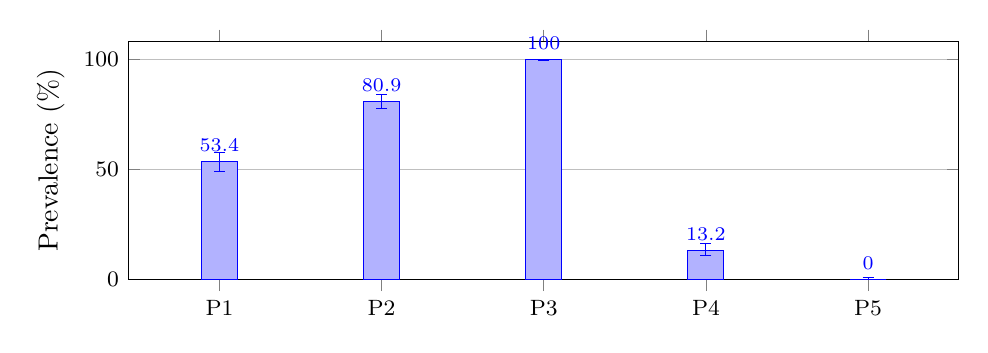
\begin{tikzpicture}
\begin{axis}[
  ybar, bar width=13pt,
  width=\linewidth, height=4.6cm,
  ymin=0, ymax=108, ylabel={Prevalence (\%)},
  symbolic x coords={P1,P2,P3,P4,P5},
  xtick=data, enlarge x limits=0.14,
  nodes near coords, nodes near coords align={vertical},
  every node near coord/.append style={font=\scriptsize},
  ymajorgrids, tick label style={font=\footnotesize},
]
% asymmetric explicit errors:  += (0, upper)  -= (0, lower)
\addplot+[error bars/.cd, y dir=both, y explicit]
coordinates {
  (P1,53.4)  += (0,4.2)  -= (0,4.3)
  (P2,80.9)  += (0,3.2)  -= (0,3.5)
  (P3,100.0) += (0,0.0)  -= (0,0.7)
  (P4,13.2)  += (0,3.2)  -= (0,2.6)
  (P5,0.0)   += (0,0.7)  -= (0,0.0)
};
\end{axis}
\end{tikzpicture}
\caption{Prevalence of cited verification weaknesses across 530 distinct
JWT-validating configurations, with Wilson 95\% confidence intervals.
P1 unbound audience; P2 no required claims; P3 no algorithm pinning \emph{in
configuration} (library-default caveat, \S\ref{sec:results}); P4 multi-issuer
(descriptive); P5 clock skew $>5$\,min (now read from Envoy
\texttt{clock\_skew\_seconds}; the widest observed is 60\,s). An independently
validated extractor; a hand-labelled gold standard is still pending
(\S\ref{sec:limitations}).}
\label{fig:prevalence}
\end{figure}

\noindent\textbf{Drift (RQ: how contracts change over time).}
Longitudinal analysis over commit history is future work. Today we validate the
drift \emph{classifier} on a 1{,}226-pair synthetic corpus at 100\% recall / 0\%
FPR, with mutation testing (24 mutants, 100\% killed) and a held-out adversarial
set at Youden 0.75. \gate{Drift in the wild, over real commit histories, is left to
the full study.}

\section{Limitations and threats to validity}\label{sec:limitations}
\textbf{Declared, not effective.} We measure the contract configuration declares,
not what the running verifier enforces. A configured check can still be skipped by
buggy verifier code, and a check absent from configuration can still hold because a
library default supplies it; conversely an implementation flaw (accepting
\texttt{alg=none}, RS/HS confusion) is invisible to us. We therefore report an
absent check as ``not set in configuration,'' not as a confirmed vulnerability, and
closing this gap needs live probing or a library-defaults database, which we leave
to future work. \textbf{Profile dependence.} Which checks are mandatory depends on
the token profile: audience and issuer validation are required for RFC~9068 access
tokens but optional for a bare RFC~7519 JWT, so an ``unbound audience'' is a
weakness only under a profile that requires binding; we measure the configured check
and name the profile where the corpus reveals it. \textbf{Templating:} $\approx$13\% of corpus files are
Helm-templated and $\approx$8\% carry kustomize/variable markers, so roughly one in
five configurations is under-resolved without rendering. \textbf{Selection bias:}
public configuration skews to samples, demos, and OSS and is not representative of
private enterprise deployments; this must be stated, not hidden. \textbf{Proxy
oracles:} \S\ref{sec:validation}'s recall/precision are automated approximations
pending human labels. \textbf{Ethics:} we use only public configuration, read
only; we do not probe third-party live endpoints and handle no real tokens;
identifiable high-severity findings follow responsible disclosure.

\section{Related work}\label{sec:related}
\noindent\textbf{In-the-wild web-authentication and SSO measurement.} The closest
line of work measures deployed authentication. Early studies inspect a small set of
sites by hand and show that SSO and OAuth failures are driven by deployment and
implementation choices rather than protocol flaws~\cite{authzmeas2012wangsignmein,authzmeas2012sunoauth}.
Later work makes this a population measurement: SSOScan automatically tests a fixed
catalog of five SSO vulnerabilities across the top 20{,}000 sites and finds that over
20\% of Facebook-SSO sites carry a serious flaw~\cite{authzmeas2014ssoscan}, and
subsequent studies measure sign-off and session handling, dual-window SSO, and SSO
adoption across the Tranco list~\cite{authzmeas2018singlesignoff,authzmeas2022distinct,authzmeas2023ssomonitor};
the OpenID Connect attack classes are systematized by Mainka et al.~\cite{authzmeas2017soksso}.
SSOScan is our closest methodological ancestor: automated detection of a fixed
weakness catalog over a crawled population. We keep that ambition but change the
object and the vantage point. We read the declared verification contract out of
static mesh and proxy configuration rather than driving a runtime login flow, which
reaches services no crawler can log into and separates what a service declares from
what it enforces.

\noindent\textbf{Large-scale misconfiguration measurement.} Our methodology follows
a well-established template: crawl a population, report the prevalence of a concrete
weakness, and quantify uncertainty. Studies of the HTTPS certificate ecosystem and
of Heartbleed turn repeated scans into a structured prevalence
picture~\cite{authzmeas2013httpsecosystem,authzmeas2014heartbleed}; the email-delivery
study measures adoption of \emph{declared} security policies (SPF, DKIM, DMARC)
across more than 700{,}000 servers~\cite{authzmeas2015emaildelivery}; and studies of
HTTPS adoption, Content Security Policy, CORS, and S3 buckets measure how a declared
per-service policy is set or fails at scale~\cite{authzmeas2017httpsadoption,authzmeas2016csp,authzmeas2018cors,authzmeas2018s3buckets}.
We adopt this template, including confidence intervals and a replication-style
validation of recall and precision, and apply it to a surface none of these touch,
the JWT authorization contract.

\noindent\textbf{IaC and configuration security.} Repository-mining studies quantify
security weaknesses in declarative infrastructure code: the Seven Sins study derives
smells from 1{,}726 scripts and counts occurrences across hundreds of
repositories~\cite{authzmeas2019sevensins}, replicated at larger scale and across
technologies~\cite{authzmeas2021iacreplication,authzmeas2022glitch}, and Kubernetes
security practice is systematized separately~\cite{authzmeas2020k8scommandments}.
Practitioner scanners (Checkov, KICS, Terrascan, Semgrep) and policy-as-code
engines~\cite{authzmeas2024checkov,authzmeas2024kics,authzmeas2024terrascan,authzmeas2024semgrep,authzmeas2024opa}
apply rule sets to individual files. These target generic hygiene (hard-coded
secrets, weak crypto) and check rules per file; we instead normalize heterogeneous
mesh and proxy configuration into one typed authorization contract per service and
measure its properties, and our negative control targets the attribution errors that
per-file pattern-matching is prone to.

\noindent\textbf{Formal analysis and config-as-contract.} A body of formal and
attack analysis establishes \emph{which} issuer, audience, algorithm, and endpoint
behaviours are load-bearing, for SAML, OAuth, and OpenID
Connect~\cite{authzmeas2008samlsso,authzmeas2012websanalysis,authzmeas2016oauthformal,authzmeas2017oidcformal};
the concrete JWT weaknesses we count (\texttt{alg=none}, RS/HS key confusion) are
documented by practitioners~\cite{authzmeas2015jwtlibs,authzmeas2024portswiggerjwt}
and codified in RFC~8725~\cite{rfc8725}. We cite these for the properties and then
measure how often deployments violate them rather than re-arguing relevance. The
idea of deriving a policy model from static configuration has a precedent in Batfish,
which parses heterogeneous device configuration into a vendor-independent model and
checks properties over it~\cite{authzmeas2015batfish}, and in ABAC policy
mining~\cite{authzmeas2015abacmining}; consumer-driven contract testing (Pact) shares
the ``contract'' framing~\cite{authzmeas2024pact}. None recovers a JWT authorization
contract or measures one across a population.

\noindent\textbf{Agent and MCP authorization.} Indirect prompt injection makes
token-scoped, verifiable authorization necessary for autonomous
agents~\cite{authzmeas2023promptinjection}, and recent measurements of live remote
MCP servers report widespread missing authentication and OAuth
flaws~\cite{authzmeas2026mcpauthmeas,authzmeas2026mcpexposed}. These show the same
population-measurement method reaching the agent frontier, where the declared-versus-effective
contract framing of this paper is the natural lens to carry forward.

\section{Future work}\label{sec:future}
Three extensions follow directly. (i) Pairing the static reading with live probing
would close the declared-vs-effective gap this paper is careful to leave open,
turning ``not set in configuration'' into a confirmed runtime behaviour. (ii) The
content-addressed contract makes \emph{drift} measurable over commit history: do
contracts widen more than they narrow, and are widenings tied to reviewable events?
(iii) The same instrument extends to the agent and MCP frontier, where OAuth/MCP
tokens carry the same issuer, audience, and claim checks on a faster-moving surface.

\section{Conclusion}
A service's decision to accept a token is configuration, declared across meshes,
proxies, and identity providers and rarely collected in one place. We make that
declared authorization contract an object that can be derived, measured, versioned,
and validated, we separate it from the effective enforcement that configuration
cannot show, and we measure it across 2{,}718 repositories with a methodology
honest about its own limits. The instrument and corpus are released so the
measurement is reproducible and extensible.

\section*{Ethics considerations}\label{sec:ethics}
This study measures only \emph{public} configuration, fetched read-only at pinned
commits, and never probes third-party live endpoints or handles real tokens; the
attack surface it characterises is exercised only against local, self-owned
negative-control fixtures. We report \emph{population} prevalence, never a verdict
on any single project, and we name no project as insecure. For any identifiable,
high-severity finding tied to a specific owner we follow coordinated responsible
disclosure before publication, allowing reasonable remediation time. The corpus
respects source licences (recorded per artifact) and robots/rate-limit norms of the
hosting platform. We see no human-subjects concerns; no personal data is collected.

\section*{Open science}\label{sec:openscience}
In keeping with open-science expectations, we release the discovery instrument, the
measurement harness (prevalence with Wilson CIs), the kind-aware validator, the
non-circular negative-control precision test, the analysis scripts, and the corpus
\emph{manifest} (repository + commit SHA + licence per artifact) so the measurement
is reproducible from public sources. \gate{At camera-ready we will add a DOI-pinned
archival snapshot and, where the venue offers it, Artifact-Evaluation ``Available'' and
``Reproduced'' badges.}

\section*{Artifact availability}\label{sec:artifact}
The instrument, harness, validator, negative-control test, and corpus manifest are
open source under the MIT licence. \gate{The archival DOI will be added at
camera-ready.}
. Every unfinished number is wrapped in \gate{...}.
% Submission vs. working-copy rendering. Default: submission (clean prose). A
% wrapper can predefine \submissionfalse before % Shared body for the Paper A measurement study. Class-agnostic: the per-venue
% main.tex sets \documentclass, title, authors, and \begin{document}, then
% % Shared body for the Paper A measurement study. Class-agnostic: the per-venue
% main.tex sets \documentclass, title, authors, and \begin{document}, then
% \input{../common/body}. Every unfinished number is wrapped in \gate{...}.
% Submission vs. working-copy rendering. Default: submission (clean prose). A
% wrapper can predefine \submissionfalse before \input{../common/body} to bring
% back the loud [PENDING]/[NOTE] markers for internal tracking.
\ifdefined\ifsubmission\else\expandafter\newif\csname ifsubmission\endcsname\submissiontrue\fi
% \gate{...}: forward-looking text. Submission -> plain prose; draft -> [PENDING].
% Content is written to read as a finished future-work sentence either way.
\providecommand{\gate}[1]{\ifsubmission #1\else \textbf{[PENDING: #1]}\fi}
% \draftonly{...}: internal note. Submission -> nothing; draft -> [NOTE].
\providecommand{\draftonly}[1]{\ifsubmission\else \textbf{[NOTE: #1]}\fi}
% Let TeX relax line breaking on paragraphs with long unbreakable \texttt{} kind
% names (RequestAuthentication, AuthorizationPolicy) instead of overrunning the
% margin. Class-agnostic; applies under every venue wrapper.
\emergencystretch=3em

% The abstract lives in common/abstract.tex. acmart requires it BEFORE \maketitle,
% llncs/IEEEtran after, so an acmart wrapper \inputs it itself (and defines
% \keywayabstractdone); every other wrapper lets the body emit it here.
\ifdefined\keywayabstractdone\else\input{abstract}\fi

\section{Introduction}
An engineer rotates a signing key on a Friday. No code changes; every test passes.
By Monday a downstream service is rejecting every valid user, because its verifier
cached the retired key longer than anyone realised. The same week, elsewhere, a
verifier quietly begins accepting a second audience nobody intended. Neither
failure lives in the code, and neither would be caught by reading it: both live in
the \emph{configuration} that actually decides whether a bearer token is accepted.

That configuration is an implicit specification: the issuers a verifier trusts,
the audiences it binds to, the algorithms it allows, the claims it requires, and
the JWKS behaviour of the library beneath it. We call it the \emph{authorization
contract}. It is spread across service meshes, proxies, identity providers, and
library defaults, it is almost never centralised, and it \emph{drifts}: a rotated
key, a widened audience, or a dropped claim turns valid users away (an outage) or
admits tokens that should be refused (a silent regression). As autonomous agents
begin carrying OAuth/MCP tokens on a user's behalf, the same contract now governs a
faster-moving, higher-stakes surface.

A caveat shapes the whole paper. What configuration states is the \emph{declared}
contract; whether a request is ultimately accepted is the \emph{effective}
behaviour, which also depends on the verifier's code, its library's defaults, and
its software version. A verifier may, for example, accept the \texttt{none}
algorithm because of an implementation flaw even where configuration says nothing,
and that is not visible in configuration at all. We measure the declared contract,
we say so throughout, and \S\ref{sec:background} and \S\ref{sec:limitations} make
the boundary between declared and effective explicit; where a declared value is
absent we distinguish ``not set in configuration'' from ``not enforced.''

This declared contract is where much of auth correctness is decided, and yet almost
nobody measures it at scale. Two kinds of tooling exist and neither answers ``what
do deployed authorization contracts look like across a population, and how healthy
are they?'' Static code scanners reason about source, not about which configured
verifier trusts which issuer; gateways and identity providers are the thing being
configured, so they do not tell an operator whether that configuration is healthy.

\noindent\textbf{Contributions.}
(i) We define the \emph{authorization contract} and give a method that derives it
from heterogeneous deployment configuration (Istio, Envoy, OIDC) with per-field
provenance and content-addressed versioning, separating the declared contract from
effective enforcement (\S\ref{sec:method}).
(ii) We measure how common concrete, normatively grounded weaknesses are across
2{,}718 public repositories and 530 JWT-validating configurations, with confidence
intervals and a co-occurrence analysis (\S\ref{sec:results}).
(iii) We give a validation methodology that is explicit about its own limits:
recall against an independent parse, a non-circular negative control for precision,
and a held-out over-attribution split, each with its failure mode stated
(\S\ref{sec:validation}).
(iv) We release the instrument, the corpus manifest, and the analysis so the study
is reproducible from public sources (\S\ref{sec:artifact}).

\section{Background}\label{sec:background}

\noindent\textbf{JWT verification.} A JSON Web Token is a signed statement of
claims: a header naming the signing algorithm, a payload of claims (including
\texttt{iss}, the issuer; \texttt{aud}, the intended audience; \texttt{exp}, the
expiry), and a signature. To accept a token, a verifier must (1) fetch the issuer's
public keys, in practice from a JSON Web Key Set (JWKS) endpoint, and verify the
signature; (2) check that \texttt{iss} is a trusted issuer; (3) check that
\texttt{aud} names this resource; (4) accept only an allow-list of signing
algorithms; and (5) enforce any additional required claims (roles, scopes, tenant).
Each step has a normative source. RFC~8725 (JSON Web Token Best Current Practices)
requires an explicit algorithm allow-list (\S3.1) and validation of all security
claims (\S3.9); RFC~9068 profiles JWT \emph{access tokens} and makes audience and
issuer validation mandatory for that profile; RFC~8707 (resource indicators) and
RFC~9728 (protected-resource metadata) bind a token to the resource it was minted
for. Which checks are mandatory therefore depends partly on the token profile in
use, a point we return to in \S\ref{sec:limitations}.

\noindent\textbf{Where the contract lives.} Few services implement these checks in
application code. In a service mesh the checks are declared as configuration and
enforced by a sidecar or gateway. Under Istio, a \texttt{RequestAuthentication}
resource declares the issuer, the JWKS source, and the accepted audiences, while an
\texttt{AuthorizationPolicy} declares required claims as \texttt{when} conditions on
\texttt{request.auth.claims[...]}; under Envoy, a \texttt{jwt\_authn} filter carries
the providers, audiences, and clock-skew tolerance. These resources usually live in
\emph{different files}, and the effective contract for one workload is their union.
Figure~\ref{fig:example} shows a minimal pair.

\begin{figure}[t]
\footnotesize
\begin{verbatim}
kind: RequestAuthentication      # issuer + audience
spec:
  selector: {matchLabels: {app: orders}}
  jwtRules:
  - issuer: "https://idp.example/realms/main"
    jwksUri: "https://idp.example/jwks.json"
    audiences: ["orders-api"]
---
kind: AuthorizationPolicy        # a required claim
spec:
  selector: {matchLabels: {app: orders}}
  rules:
  - when:
    - key: request.auth.claims[groups]
      values: ["ops"]
\end{verbatim}
\caption{The declared authorization contract for the \texttt{orders} workload,
spread across two resources: trust \texttt{idp.example}, require audience
\texttt{orders-api}, and require a \texttt{groups} claim of \texttt{ops}. No signing
algorithm is pinned, so the mesh applies its library default (\S\ref{sec:results}).}
\label{fig:example}
\end{figure}

\noindent\textbf{Declared vs.\ effective; terminology.} We measure the
\emph{declared} contract in resources like these. The \emph{effective} behaviour
can differ: a verifier might skip a check, honour a dangerous default, or carry an
implementation bug (accepting \texttt{alg=none}, confusing RS256 and HS256). Those
are code, not configuration, and outside the reach of a static reading; we flag the
absence of a configured check as ``not set in configuration,'' never as a confirmed
runtime vulnerability. We use \emph{consumer} for the verifying entity a contract
belongs to (an Istio workload, an Envoy route), and we restrict \emph{authorization
contract} to \emph{token validation} (is this token acceptable?), as distinct from
resource-level authorization (may this subject perform this action?), which is a
separate layer we do not measure.

\section{Deriving authorization contracts}\label{sec:method}
We derive one contract per \emph{consumer} (\S\ref{sec:background}) from the
configuration that governs it. Source-specific \emph{discoverers} parse each format
(Istio \texttt{RequestAuthentication} and \texttt{AuthorizationPolicy}, Envoy
\texttt{jwt\_authn}, and OIDC/Keycloak registries) into a common contract of
issuers, audiences, algorithms, required claims, and JWKS behaviour.

Deriving a contract is not a one-resource read, because the checks are split across
resources (\S\ref{sec:background}). For the pair in Figure~\ref{fig:example}, the
\texttt{RequestAuthentication} contributes the issuer, JWKS source, and audience,
and the \texttt{AuthorizationPolicy} contributes the required \texttt{groups} claim;
we join them by the workload they select (\texttt{app: orders}) into a single
consumer whose contract carries all three. Attribution follows the mesh's own
semantics: a selector-less policy applies to every workload in its namespace, and
in a namespace with a single JWT consumer a per-service claim policy attaches to
that consumer (the common edge-gateway pattern). The same join resolves audiences
declared in an \texttt{AuthorizationPolicy} condition on
\texttt{request.auth.audiences} rather than in the \texttt{RequestAuthentication}.

Every extracted field records \emph{provenance}: the source kind, the file
locator, and a confidence. Each measurement is therefore attributable to a line of
configuration and a human can check it (we use this in \S\ref{sec:validation}).
A library-defaults database records what a verifier does when configuration is
silent, kept separate from what configuration states so the two are never conflated.
Consumers are assembled into a content-addressed \texttt{ContractVersion}, which
makes change detection exact equality and lets us diff one deployment's contract
against another or against its own history.

\section{Corpus construction}\label{sec:corpus}
We crawl public GitHub read-only for real auth configuration (Istio
\texttt{RequestAuthentication}, Envoy \texttt{jwt\_authn}, Istio claim conditions),
recording repository, blob SHA, and licence for every artifact for reproducibility
and attribution. We fetch public repositories only, cap files per repository to
limit monorepo dominance, and analyse \emph{per repository} so a
\texttt{RequestAuthentication} and its \texttt{AuthorizationPolicy} (usually in
separate files) are resolved together while distinct repositories remain isolated.
Two cleaning steps address representativeness: we exclude tutorial/vendored copies
by path (matched against the full locator, so \texttt{testdata/}, \texttt{vendor/},
and \texttt{/e2e/} components are caught, not only basenames), and we deduplicate
identical configurations (a canonical sample pasted across repositories counts
once). The corpus is 5{,}214 files across 2{,}718 public repositories, yielding 778
JWT-validating configurations, or 530 after deduplication. \gate{A full study will
push the corpus further toward $10^4$ services, add OIDC/MCP sources, and report a
selection-bias analysis against the public-configuration population.}

\section{Validation methodology}\label{sec:validation}
Measurement is only as good as the extractor. We validate discovery three ways, for
recall, for precision, and for over-attribution, and are explicit about what each
can and cannot establish.

\noindent\textbf{Recall (kind-aware independent parse).} An independent YAML parse
of each repository yields the declared issuers/audiences/claims; we compare to what
discovery captured, per repository. The independent parser also
\emph{over-declares}: it scrapes \texttt{issuer:} keys and claim-like strings from
non-auth resources (a ConfigMap, an annotation). We therefore measure recall only
against values in \emph{genuine} auth resources (RequestAuthentication /
AuthorizationPolicy / Envoy JWT). Adjudicated recall is issuers 96.0\%, audiences
98.2\%, and claims 86.0\% (scoped to repositories where a JWT consumer exists;
claims declared in repositories whose RequestAuthentication is absent from the
corpus have no consumer to attach to). The adjudication removed 106 parser
over-declarations (65 issuers, 27 audiences, 14 claims), which both raises the
honest recall and demonstrates the proxy oracle is itself imperfect. The issuer
figure rose from an earlier 89.6\% once a document-splitting bug was fixed: a single
templated or malformed YAML document had been aborting the rest of its file, so the
earlier recall was depressed by the extractor, not by the corpus.

\noindent\textbf{Precision (non-circular negative control).} An independent-parse
oracle cannot honestly measure precision: it reads the same fields as the
extractor, so captures are almost always a subset and precision $\approx 100\%$
\emph{by construction}. We therefore use a negative control: configurations with
planted distractor values a correct discoverer must ignore: a commented-out
issuer, an \texttt{issuer:}/claim in a non-auth ConfigMap, a claim behind a
non-matching AuthorizationPolicy selector (the real attribution risk), and strings
in annotations. Result: 4 planted, 0 leaked, with real values still captured.

\noindent\textbf{Over-attribution (held-out split).} To measure how often discovery
\emph{adds} a value that is not really there, we take every captured/declared
disagreement, label each with an independent model that reads only the raw
configuration and never the extractor's output (so the grading is non-circular),
and split the labelled set 70/30 by repository so no repository informs both sides.
On the held-out test split, precision is 100\% and over-attribution is 0.0\% (0 of 6
captured-only values are spurious or mis-attributed); on the full labelled set,
precision 100\% and over-attribution 0.0\%. This split is what caught, and then
confirmed the fix for, an Envoy test-fixture leak and a claim mis-attribution during
development.

\noindent\textbf{Gold standard.} All three above are automated or model-assisted
proxies. For a population-level ground truth we draw a stratified random sample of
401 \mbox{(repo, field, value)} rows across the corpus, powered for a $\pm$1.8\%
precision and $\pm$2.4\% recall confidence interval, and have each adjudicated by
hand as real, correctly attributed, or spurious; a model drafts a first-pass label
that the human confirms or corrects, and a blind subset gives an un-anchored
inter-annotator agreement (Cohen's $\kappa$). \gate{We report the hand-validated
precision, recall, and $\kappa$ in the final version; the automated results above
are what the gold standard refines.}

\section{Results}\label{sec:results}
We report prevalence over the 530 deduplicated JWT-validating configurations, each
with a 95\% Wilson confidence interval (the Wilson interval is preferred over the
normal approximation for proportions near 0 or 1). These figures come from the
independently validated extractor of \S\ref{sec:validation}; the hand-validated
gold standard refines the \emph{validation} numbers, not the prevalence below.

\noindent\textbf{Prevalence.} Over 530 distinct JWT-validating configurations
(Wilson 95\% CIs): no algorithm pinning \emph{in configuration} 100\%
[99.3, 100]; no required claims 80.9\% [77.4, 84.1]; unbound audience 53.4\%
[49.1, 57.6]; multi-issuer trust 13.2\% [10.6, 16.4] (descriptive, not a weakness);
clock skew $>5$\,min 0.0\% [0.0, 0.7]. The algorithm-pinning figure reflects
reliance on the verifying \emph{library's default}, which configuration does not
restate. This is a static-vs-runtime gap, not a 100\% vulnerability rate; we report
it as ``not pinned in config.'' The clock-skew figure is now read directly from
Envoy \texttt{clock\_skew\_seconds} rather than assumed: of the configurations that
set it the widest is 60\,s, so the 0.0\% above the 5-minute threshold is measured,
not merely unobserved. The earlier draft's 42.2\% unbound-audience figure, over a
102-configuration pilot, rises to 53.4\% on this larger and more representative
corpus; the direction and the majority finding are unchanged.

\noindent\textbf{Co-occurrence.} Weaknesses travel together. No-required-claims and
no-algorithm-pinning co-occur in 80.9\% of configurations; unbound-audience with
no-algorithm-pinning in 53.4\%; unbound-audience with no-required-claims in 43.8\%
(lift $\approx$1.0, i.e. roughly independent rather than mutually reinforcing).

\noindent\textbf{Static/runtime frontier.} Four of the five check types are
conclusive from configuration alone; only algorithm pinning carries the
library-default caveat. Of 1{,}312 weakness flags raised, 782 (60\%) are
static-conclusive and 530 carry that caveat, quantifying how much of the contract a
purely static reading can settle.

\input{../common/fig-prevalence}

\noindent\textbf{Drift (RQ: how contracts change over time).}
Longitudinal analysis over commit history is future work. Today we validate the
drift \emph{classifier} on a 1{,}226-pair synthetic corpus at 100\% recall / 0\%
FPR, with mutation testing (24 mutants, 100\% killed) and a held-out adversarial
set at Youden 0.75. \gate{Drift in the wild, over real commit histories, is left to
the full study.}

\section{Limitations and threats to validity}\label{sec:limitations}
\textbf{Declared, not effective.} We measure the contract configuration declares,
not what the running verifier enforces. A configured check can still be skipped by
buggy verifier code, and a check absent from configuration can still hold because a
library default supplies it; conversely an implementation flaw (accepting
\texttt{alg=none}, RS/HS confusion) is invisible to us. We therefore report an
absent check as ``not set in configuration,'' not as a confirmed vulnerability, and
closing this gap needs live probing or a library-defaults database, which we leave
to future work. \textbf{Profile dependence.} Which checks are mandatory depends on
the token profile: audience and issuer validation are required for RFC~9068 access
tokens but optional for a bare RFC~7519 JWT, so an ``unbound audience'' is a
weakness only under a profile that requires binding; we measure the configured check
and name the profile where the corpus reveals it. \textbf{Templating:} $\approx$13\% of corpus files are
Helm-templated and $\approx$8\% carry kustomize/variable markers, so roughly one in
five configurations is under-resolved without rendering. \textbf{Selection bias:}
public configuration skews to samples, demos, and OSS and is not representative of
private enterprise deployments; this must be stated, not hidden. \textbf{Proxy
oracles:} \S\ref{sec:validation}'s recall/precision are automated approximations
pending human labels. \textbf{Ethics:} we use only public configuration, read
only; we do not probe third-party live endpoints and handle no real tokens;
identifiable high-severity findings follow responsible disclosure.

\section{Related work}\label{sec:related}
\noindent\textbf{In-the-wild web-authentication and SSO measurement.} The closest
line of work measures deployed authentication. Early studies inspect a small set of
sites by hand and show that SSO and OAuth failures are driven by deployment and
implementation choices rather than protocol flaws~\cite{authzmeas2012wangsignmein,authzmeas2012sunoauth}.
Later work makes this a population measurement: SSOScan automatically tests a fixed
catalog of five SSO vulnerabilities across the top 20{,}000 sites and finds that over
20\% of Facebook-SSO sites carry a serious flaw~\cite{authzmeas2014ssoscan}, and
subsequent studies measure sign-off and session handling, dual-window SSO, and SSO
adoption across the Tranco list~\cite{authzmeas2018singlesignoff,authzmeas2022distinct,authzmeas2023ssomonitor};
the OpenID Connect attack classes are systematized by Mainka et al.~\cite{authzmeas2017soksso}.
SSOScan is our closest methodological ancestor: automated detection of a fixed
weakness catalog over a crawled population. We keep that ambition but change the
object and the vantage point. We read the declared verification contract out of
static mesh and proxy configuration rather than driving a runtime login flow, which
reaches services no crawler can log into and separates what a service declares from
what it enforces.

\noindent\textbf{Large-scale misconfiguration measurement.} Our methodology follows
a well-established template: crawl a population, report the prevalence of a concrete
weakness, and quantify uncertainty. Studies of the HTTPS certificate ecosystem and
of Heartbleed turn repeated scans into a structured prevalence
picture~\cite{authzmeas2013httpsecosystem,authzmeas2014heartbleed}; the email-delivery
study measures adoption of \emph{declared} security policies (SPF, DKIM, DMARC)
across more than 700{,}000 servers~\cite{authzmeas2015emaildelivery}; and studies of
HTTPS adoption, Content Security Policy, CORS, and S3 buckets measure how a declared
per-service policy is set or fails at scale~\cite{authzmeas2017httpsadoption,authzmeas2016csp,authzmeas2018cors,authzmeas2018s3buckets}.
We adopt this template, including confidence intervals and a replication-style
validation of recall and precision, and apply it to a surface none of these touch,
the JWT authorization contract.

\noindent\textbf{IaC and configuration security.} Repository-mining studies quantify
security weaknesses in declarative infrastructure code: the Seven Sins study derives
smells from 1{,}726 scripts and counts occurrences across hundreds of
repositories~\cite{authzmeas2019sevensins}, replicated at larger scale and across
technologies~\cite{authzmeas2021iacreplication,authzmeas2022glitch}, and Kubernetes
security practice is systematized separately~\cite{authzmeas2020k8scommandments}.
Practitioner scanners (Checkov, KICS, Terrascan, Semgrep) and policy-as-code
engines~\cite{authzmeas2024checkov,authzmeas2024kics,authzmeas2024terrascan,authzmeas2024semgrep,authzmeas2024opa}
apply rule sets to individual files. These target generic hygiene (hard-coded
secrets, weak crypto) and check rules per file; we instead normalize heterogeneous
mesh and proxy configuration into one typed authorization contract per service and
measure its properties, and our negative control targets the attribution errors that
per-file pattern-matching is prone to.

\noindent\textbf{Formal analysis and config-as-contract.} A body of formal and
attack analysis establishes \emph{which} issuer, audience, algorithm, and endpoint
behaviours are load-bearing, for SAML, OAuth, and OpenID
Connect~\cite{authzmeas2008samlsso,authzmeas2012websanalysis,authzmeas2016oauthformal,authzmeas2017oidcformal};
the concrete JWT weaknesses we count (\texttt{alg=none}, RS/HS key confusion) are
documented by practitioners~\cite{authzmeas2015jwtlibs,authzmeas2024portswiggerjwt}
and codified in RFC~8725~\cite{rfc8725}. We cite these for the properties and then
measure how often deployments violate them rather than re-arguing relevance. The
idea of deriving a policy model from static configuration has a precedent in Batfish,
which parses heterogeneous device configuration into a vendor-independent model and
checks properties over it~\cite{authzmeas2015batfish}, and in ABAC policy
mining~\cite{authzmeas2015abacmining}; consumer-driven contract testing (Pact) shares
the ``contract'' framing~\cite{authzmeas2024pact}. None recovers a JWT authorization
contract or measures one across a population.

\noindent\textbf{Agent and MCP authorization.} Indirect prompt injection makes
token-scoped, verifiable authorization necessary for autonomous
agents~\cite{authzmeas2023promptinjection}, and recent measurements of live remote
MCP servers report widespread missing authentication and OAuth
flaws~\cite{authzmeas2026mcpauthmeas,authzmeas2026mcpexposed}. These show the same
population-measurement method reaching the agent frontier, where the declared-versus-effective
contract framing of this paper is the natural lens to carry forward.

\section{Future work}\label{sec:future}
Three extensions follow directly. (i) Pairing the static reading with live probing
would close the declared-vs-effective gap this paper is careful to leave open,
turning ``not set in configuration'' into a confirmed runtime behaviour. (ii) The
content-addressed contract makes \emph{drift} measurable over commit history: do
contracts widen more than they narrow, and are widenings tied to reviewable events?
(iii) The same instrument extends to the agent and MCP frontier, where OAuth/MCP
tokens carry the same issuer, audience, and claim checks on a faster-moving surface.

\section{Conclusion}
A service's decision to accept a token is configuration, declared across meshes,
proxies, and identity providers and rarely collected in one place. We make that
declared authorization contract an object that can be derived, measured, versioned,
and validated, we separate it from the effective enforcement that configuration
cannot show, and we measure it across 2{,}718 repositories with a methodology
honest about its own limits. The instrument and corpus are released so the
measurement is reproducible and extensible.

\section*{Ethics considerations}\label{sec:ethics}
This study measures only \emph{public} configuration, fetched read-only at pinned
commits, and never probes third-party live endpoints or handles real tokens; the
attack surface it characterises is exercised only against local, self-owned
negative-control fixtures. We report \emph{population} prevalence, never a verdict
on any single project, and we name no project as insecure. For any identifiable,
high-severity finding tied to a specific owner we follow coordinated responsible
disclosure before publication, allowing reasonable remediation time. The corpus
respects source licences (recorded per artifact) and robots/rate-limit norms of the
hosting platform. We see no human-subjects concerns; no personal data is collected.

\section*{Open science}\label{sec:openscience}
In keeping with open-science expectations, we release the discovery instrument, the
measurement harness (prevalence with Wilson CIs), the kind-aware validator, the
non-circular negative-control precision test, the analysis scripts, and the corpus
\emph{manifest} (repository + commit SHA + licence per artifact) so the measurement
is reproducible from public sources. \gate{At camera-ready we will add a DOI-pinned
archival snapshot and, where the venue offers it, Artifact-Evaluation ``Available'' and
``Reproduced'' badges.}

\section*{Artifact availability}\label{sec:artifact}
The instrument, harness, validator, negative-control test, and corpus manifest are
open source under the MIT licence. \gate{The archival DOI will be added at
camera-ready.}
. Every unfinished number is wrapped in \gate{...}.
% Submission vs. working-copy rendering. Default: submission (clean prose). A
% wrapper can predefine \submissionfalse before % Shared body for the Paper A measurement study. Class-agnostic: the per-venue
% main.tex sets \documentclass, title, authors, and \begin{document}, then
% \input{../common/body}. Every unfinished number is wrapped in \gate{...}.
% Submission vs. working-copy rendering. Default: submission (clean prose). A
% wrapper can predefine \submissionfalse before \input{../common/body} to bring
% back the loud [PENDING]/[NOTE] markers for internal tracking.
\ifdefined\ifsubmission\else\expandafter\newif\csname ifsubmission\endcsname\submissiontrue\fi
% \gate{...}: forward-looking text. Submission -> plain prose; draft -> [PENDING].
% Content is written to read as a finished future-work sentence either way.
\providecommand{\gate}[1]{\ifsubmission #1\else \textbf{[PENDING: #1]}\fi}
% \draftonly{...}: internal note. Submission -> nothing; draft -> [NOTE].
\providecommand{\draftonly}[1]{\ifsubmission\else \textbf{[NOTE: #1]}\fi}
% Let TeX relax line breaking on paragraphs with long unbreakable \texttt{} kind
% names (RequestAuthentication, AuthorizationPolicy) instead of overrunning the
% margin. Class-agnostic; applies under every venue wrapper.
\emergencystretch=3em

% The abstract lives in common/abstract.tex. acmart requires it BEFORE \maketitle,
% llncs/IEEEtran after, so an acmart wrapper \inputs it itself (and defines
% \keywayabstractdone); every other wrapper lets the body emit it here.
\ifdefined\keywayabstractdone\else\input{abstract}\fi

\section{Introduction}
An engineer rotates a signing key on a Friday. No code changes; every test passes.
By Monday a downstream service is rejecting every valid user, because its verifier
cached the retired key longer than anyone realised. The same week, elsewhere, a
verifier quietly begins accepting a second audience nobody intended. Neither
failure lives in the code, and neither would be caught by reading it: both live in
the \emph{configuration} that actually decides whether a bearer token is accepted.

That configuration is an implicit specification: the issuers a verifier trusts,
the audiences it binds to, the algorithms it allows, the claims it requires, and
the JWKS behaviour of the library beneath it. We call it the \emph{authorization
contract}. It is spread across service meshes, proxies, identity providers, and
library defaults, it is almost never centralised, and it \emph{drifts}: a rotated
key, a widened audience, or a dropped claim turns valid users away (an outage) or
admits tokens that should be refused (a silent regression). As autonomous agents
begin carrying OAuth/MCP tokens on a user's behalf, the same contract now governs a
faster-moving, higher-stakes surface.

A caveat shapes the whole paper. What configuration states is the \emph{declared}
contract; whether a request is ultimately accepted is the \emph{effective}
behaviour, which also depends on the verifier's code, its library's defaults, and
its software version. A verifier may, for example, accept the \texttt{none}
algorithm because of an implementation flaw even where configuration says nothing,
and that is not visible in configuration at all. We measure the declared contract,
we say so throughout, and \S\ref{sec:background} and \S\ref{sec:limitations} make
the boundary between declared and effective explicit; where a declared value is
absent we distinguish ``not set in configuration'' from ``not enforced.''

This declared contract is where much of auth correctness is decided, and yet almost
nobody measures it at scale. Two kinds of tooling exist and neither answers ``what
do deployed authorization contracts look like across a population, and how healthy
are they?'' Static code scanners reason about source, not about which configured
verifier trusts which issuer; gateways and identity providers are the thing being
configured, so they do not tell an operator whether that configuration is healthy.

\noindent\textbf{Contributions.}
(i) We define the \emph{authorization contract} and give a method that derives it
from heterogeneous deployment configuration (Istio, Envoy, OIDC) with per-field
provenance and content-addressed versioning, separating the declared contract from
effective enforcement (\S\ref{sec:method}).
(ii) We measure how common concrete, normatively grounded weaknesses are across
2{,}718 public repositories and 530 JWT-validating configurations, with confidence
intervals and a co-occurrence analysis (\S\ref{sec:results}).
(iii) We give a validation methodology that is explicit about its own limits:
recall against an independent parse, a non-circular negative control for precision,
and a held-out over-attribution split, each with its failure mode stated
(\S\ref{sec:validation}).
(iv) We release the instrument, the corpus manifest, and the analysis so the study
is reproducible from public sources (\S\ref{sec:artifact}).

\section{Background}\label{sec:background}

\noindent\textbf{JWT verification.} A JSON Web Token is a signed statement of
claims: a header naming the signing algorithm, a payload of claims (including
\texttt{iss}, the issuer; \texttt{aud}, the intended audience; \texttt{exp}, the
expiry), and a signature. To accept a token, a verifier must (1) fetch the issuer's
public keys, in practice from a JSON Web Key Set (JWKS) endpoint, and verify the
signature; (2) check that \texttt{iss} is a trusted issuer; (3) check that
\texttt{aud} names this resource; (4) accept only an allow-list of signing
algorithms; and (5) enforce any additional required claims (roles, scopes, tenant).
Each step has a normative source. RFC~8725 (JSON Web Token Best Current Practices)
requires an explicit algorithm allow-list (\S3.1) and validation of all security
claims (\S3.9); RFC~9068 profiles JWT \emph{access tokens} and makes audience and
issuer validation mandatory for that profile; RFC~8707 (resource indicators) and
RFC~9728 (protected-resource metadata) bind a token to the resource it was minted
for. Which checks are mandatory therefore depends partly on the token profile in
use, a point we return to in \S\ref{sec:limitations}.

\noindent\textbf{Where the contract lives.} Few services implement these checks in
application code. In a service mesh the checks are declared as configuration and
enforced by a sidecar or gateway. Under Istio, a \texttt{RequestAuthentication}
resource declares the issuer, the JWKS source, and the accepted audiences, while an
\texttt{AuthorizationPolicy} declares required claims as \texttt{when} conditions on
\texttt{request.auth.claims[...]}; under Envoy, a \texttt{jwt\_authn} filter carries
the providers, audiences, and clock-skew tolerance. These resources usually live in
\emph{different files}, and the effective contract for one workload is their union.
Figure~\ref{fig:example} shows a minimal pair.

\begin{figure}[t]
\footnotesize
\begin{verbatim}
kind: RequestAuthentication      # issuer + audience
spec:
  selector: {matchLabels: {app: orders}}
  jwtRules:
  - issuer: "https://idp.example/realms/main"
    jwksUri: "https://idp.example/jwks.json"
    audiences: ["orders-api"]
---
kind: AuthorizationPolicy        # a required claim
spec:
  selector: {matchLabels: {app: orders}}
  rules:
  - when:
    - key: request.auth.claims[groups]
      values: ["ops"]
\end{verbatim}
\caption{The declared authorization contract for the \texttt{orders} workload,
spread across two resources: trust \texttt{idp.example}, require audience
\texttt{orders-api}, and require a \texttt{groups} claim of \texttt{ops}. No signing
algorithm is pinned, so the mesh applies its library default (\S\ref{sec:results}).}
\label{fig:example}
\end{figure}

\noindent\textbf{Declared vs.\ effective; terminology.} We measure the
\emph{declared} contract in resources like these. The \emph{effective} behaviour
can differ: a verifier might skip a check, honour a dangerous default, or carry an
implementation bug (accepting \texttt{alg=none}, confusing RS256 and HS256). Those
are code, not configuration, and outside the reach of a static reading; we flag the
absence of a configured check as ``not set in configuration,'' never as a confirmed
runtime vulnerability. We use \emph{consumer} for the verifying entity a contract
belongs to (an Istio workload, an Envoy route), and we restrict \emph{authorization
contract} to \emph{token validation} (is this token acceptable?), as distinct from
resource-level authorization (may this subject perform this action?), which is a
separate layer we do not measure.

\section{Deriving authorization contracts}\label{sec:method}
We derive one contract per \emph{consumer} (\S\ref{sec:background}) from the
configuration that governs it. Source-specific \emph{discoverers} parse each format
(Istio \texttt{RequestAuthentication} and \texttt{AuthorizationPolicy}, Envoy
\texttt{jwt\_authn}, and OIDC/Keycloak registries) into a common contract of
issuers, audiences, algorithms, required claims, and JWKS behaviour.

Deriving a contract is not a one-resource read, because the checks are split across
resources (\S\ref{sec:background}). For the pair in Figure~\ref{fig:example}, the
\texttt{RequestAuthentication} contributes the issuer, JWKS source, and audience,
and the \texttt{AuthorizationPolicy} contributes the required \texttt{groups} claim;
we join them by the workload they select (\texttt{app: orders}) into a single
consumer whose contract carries all three. Attribution follows the mesh's own
semantics: a selector-less policy applies to every workload in its namespace, and
in a namespace with a single JWT consumer a per-service claim policy attaches to
that consumer (the common edge-gateway pattern). The same join resolves audiences
declared in an \texttt{AuthorizationPolicy} condition on
\texttt{request.auth.audiences} rather than in the \texttt{RequestAuthentication}.

Every extracted field records \emph{provenance}: the source kind, the file
locator, and a confidence. Each measurement is therefore attributable to a line of
configuration and a human can check it (we use this in \S\ref{sec:validation}).
A library-defaults database records what a verifier does when configuration is
silent, kept separate from what configuration states so the two are never conflated.
Consumers are assembled into a content-addressed \texttt{ContractVersion}, which
makes change detection exact equality and lets us diff one deployment's contract
against another or against its own history.

\section{Corpus construction}\label{sec:corpus}
We crawl public GitHub read-only for real auth configuration (Istio
\texttt{RequestAuthentication}, Envoy \texttt{jwt\_authn}, Istio claim conditions),
recording repository, blob SHA, and licence for every artifact for reproducibility
and attribution. We fetch public repositories only, cap files per repository to
limit monorepo dominance, and analyse \emph{per repository} so a
\texttt{RequestAuthentication} and its \texttt{AuthorizationPolicy} (usually in
separate files) are resolved together while distinct repositories remain isolated.
Two cleaning steps address representativeness: we exclude tutorial/vendored copies
by path (matched against the full locator, so \texttt{testdata/}, \texttt{vendor/},
and \texttt{/e2e/} components are caught, not only basenames), and we deduplicate
identical configurations (a canonical sample pasted across repositories counts
once). The corpus is 5{,}214 files across 2{,}718 public repositories, yielding 778
JWT-validating configurations, or 530 after deduplication. \gate{A full study will
push the corpus further toward $10^4$ services, add OIDC/MCP sources, and report a
selection-bias analysis against the public-configuration population.}

\section{Validation methodology}\label{sec:validation}
Measurement is only as good as the extractor. We validate discovery three ways, for
recall, for precision, and for over-attribution, and are explicit about what each
can and cannot establish.

\noindent\textbf{Recall (kind-aware independent parse).} An independent YAML parse
of each repository yields the declared issuers/audiences/claims; we compare to what
discovery captured, per repository. The independent parser also
\emph{over-declares}: it scrapes \texttt{issuer:} keys and claim-like strings from
non-auth resources (a ConfigMap, an annotation). We therefore measure recall only
against values in \emph{genuine} auth resources (RequestAuthentication /
AuthorizationPolicy / Envoy JWT). Adjudicated recall is issuers 96.0\%, audiences
98.2\%, and claims 86.0\% (scoped to repositories where a JWT consumer exists;
claims declared in repositories whose RequestAuthentication is absent from the
corpus have no consumer to attach to). The adjudication removed 106 parser
over-declarations (65 issuers, 27 audiences, 14 claims), which both raises the
honest recall and demonstrates the proxy oracle is itself imperfect. The issuer
figure rose from an earlier 89.6\% once a document-splitting bug was fixed: a single
templated or malformed YAML document had been aborting the rest of its file, so the
earlier recall was depressed by the extractor, not by the corpus.

\noindent\textbf{Precision (non-circular negative control).} An independent-parse
oracle cannot honestly measure precision: it reads the same fields as the
extractor, so captures are almost always a subset and precision $\approx 100\%$
\emph{by construction}. We therefore use a negative control: configurations with
planted distractor values a correct discoverer must ignore: a commented-out
issuer, an \texttt{issuer:}/claim in a non-auth ConfigMap, a claim behind a
non-matching AuthorizationPolicy selector (the real attribution risk), and strings
in annotations. Result: 4 planted, 0 leaked, with real values still captured.

\noindent\textbf{Over-attribution (held-out split).} To measure how often discovery
\emph{adds} a value that is not really there, we take every captured/declared
disagreement, label each with an independent model that reads only the raw
configuration and never the extractor's output (so the grading is non-circular),
and split the labelled set 70/30 by repository so no repository informs both sides.
On the held-out test split, precision is 100\% and over-attribution is 0.0\% (0 of 6
captured-only values are spurious or mis-attributed); on the full labelled set,
precision 100\% and over-attribution 0.0\%. This split is what caught, and then
confirmed the fix for, an Envoy test-fixture leak and a claim mis-attribution during
development.

\noindent\textbf{Gold standard.} All three above are automated or model-assisted
proxies. For a population-level ground truth we draw a stratified random sample of
401 \mbox{(repo, field, value)} rows across the corpus, powered for a $\pm$1.8\%
precision and $\pm$2.4\% recall confidence interval, and have each adjudicated by
hand as real, correctly attributed, or spurious; a model drafts a first-pass label
that the human confirms or corrects, and a blind subset gives an un-anchored
inter-annotator agreement (Cohen's $\kappa$). \gate{We report the hand-validated
precision, recall, and $\kappa$ in the final version; the automated results above
are what the gold standard refines.}

\section{Results}\label{sec:results}
We report prevalence over the 530 deduplicated JWT-validating configurations, each
with a 95\% Wilson confidence interval (the Wilson interval is preferred over the
normal approximation for proportions near 0 or 1). These figures come from the
independently validated extractor of \S\ref{sec:validation}; the hand-validated
gold standard refines the \emph{validation} numbers, not the prevalence below.

\noindent\textbf{Prevalence.} Over 530 distinct JWT-validating configurations
(Wilson 95\% CIs): no algorithm pinning \emph{in configuration} 100\%
[99.3, 100]; no required claims 80.9\% [77.4, 84.1]; unbound audience 53.4\%
[49.1, 57.6]; multi-issuer trust 13.2\% [10.6, 16.4] (descriptive, not a weakness);
clock skew $>5$\,min 0.0\% [0.0, 0.7]. The algorithm-pinning figure reflects
reliance on the verifying \emph{library's default}, which configuration does not
restate. This is a static-vs-runtime gap, not a 100\% vulnerability rate; we report
it as ``not pinned in config.'' The clock-skew figure is now read directly from
Envoy \texttt{clock\_skew\_seconds} rather than assumed: of the configurations that
set it the widest is 60\,s, so the 0.0\% above the 5-minute threshold is measured,
not merely unobserved. The earlier draft's 42.2\% unbound-audience figure, over a
102-configuration pilot, rises to 53.4\% on this larger and more representative
corpus; the direction and the majority finding are unchanged.

\noindent\textbf{Co-occurrence.} Weaknesses travel together. No-required-claims and
no-algorithm-pinning co-occur in 80.9\% of configurations; unbound-audience with
no-algorithm-pinning in 53.4\%; unbound-audience with no-required-claims in 43.8\%
(lift $\approx$1.0, i.e. roughly independent rather than mutually reinforcing).

\noindent\textbf{Static/runtime frontier.} Four of the five check types are
conclusive from configuration alone; only algorithm pinning carries the
library-default caveat. Of 1{,}312 weakness flags raised, 782 (60\%) are
static-conclusive and 530 carry that caveat, quantifying how much of the contract a
purely static reading can settle.

\input{../common/fig-prevalence}

\noindent\textbf{Drift (RQ: how contracts change over time).}
Longitudinal analysis over commit history is future work. Today we validate the
drift \emph{classifier} on a 1{,}226-pair synthetic corpus at 100\% recall / 0\%
FPR, with mutation testing (24 mutants, 100\% killed) and a held-out adversarial
set at Youden 0.75. \gate{Drift in the wild, over real commit histories, is left to
the full study.}

\section{Limitations and threats to validity}\label{sec:limitations}
\textbf{Declared, not effective.} We measure the contract configuration declares,
not what the running verifier enforces. A configured check can still be skipped by
buggy verifier code, and a check absent from configuration can still hold because a
library default supplies it; conversely an implementation flaw (accepting
\texttt{alg=none}, RS/HS confusion) is invisible to us. We therefore report an
absent check as ``not set in configuration,'' not as a confirmed vulnerability, and
closing this gap needs live probing or a library-defaults database, which we leave
to future work. \textbf{Profile dependence.} Which checks are mandatory depends on
the token profile: audience and issuer validation are required for RFC~9068 access
tokens but optional for a bare RFC~7519 JWT, so an ``unbound audience'' is a
weakness only under a profile that requires binding; we measure the configured check
and name the profile where the corpus reveals it. \textbf{Templating:} $\approx$13\% of corpus files are
Helm-templated and $\approx$8\% carry kustomize/variable markers, so roughly one in
five configurations is under-resolved without rendering. \textbf{Selection bias:}
public configuration skews to samples, demos, and OSS and is not representative of
private enterprise deployments; this must be stated, not hidden. \textbf{Proxy
oracles:} \S\ref{sec:validation}'s recall/precision are automated approximations
pending human labels. \textbf{Ethics:} we use only public configuration, read
only; we do not probe third-party live endpoints and handle no real tokens;
identifiable high-severity findings follow responsible disclosure.

\section{Related work}\label{sec:related}
\noindent\textbf{In-the-wild web-authentication and SSO measurement.} The closest
line of work measures deployed authentication. Early studies inspect a small set of
sites by hand and show that SSO and OAuth failures are driven by deployment and
implementation choices rather than protocol flaws~\cite{authzmeas2012wangsignmein,authzmeas2012sunoauth}.
Later work makes this a population measurement: SSOScan automatically tests a fixed
catalog of five SSO vulnerabilities across the top 20{,}000 sites and finds that over
20\% of Facebook-SSO sites carry a serious flaw~\cite{authzmeas2014ssoscan}, and
subsequent studies measure sign-off and session handling, dual-window SSO, and SSO
adoption across the Tranco list~\cite{authzmeas2018singlesignoff,authzmeas2022distinct,authzmeas2023ssomonitor};
the OpenID Connect attack classes are systematized by Mainka et al.~\cite{authzmeas2017soksso}.
SSOScan is our closest methodological ancestor: automated detection of a fixed
weakness catalog over a crawled population. We keep that ambition but change the
object and the vantage point. We read the declared verification contract out of
static mesh and proxy configuration rather than driving a runtime login flow, which
reaches services no crawler can log into and separates what a service declares from
what it enforces.

\noindent\textbf{Large-scale misconfiguration measurement.} Our methodology follows
a well-established template: crawl a population, report the prevalence of a concrete
weakness, and quantify uncertainty. Studies of the HTTPS certificate ecosystem and
of Heartbleed turn repeated scans into a structured prevalence
picture~\cite{authzmeas2013httpsecosystem,authzmeas2014heartbleed}; the email-delivery
study measures adoption of \emph{declared} security policies (SPF, DKIM, DMARC)
across more than 700{,}000 servers~\cite{authzmeas2015emaildelivery}; and studies of
HTTPS adoption, Content Security Policy, CORS, and S3 buckets measure how a declared
per-service policy is set or fails at scale~\cite{authzmeas2017httpsadoption,authzmeas2016csp,authzmeas2018cors,authzmeas2018s3buckets}.
We adopt this template, including confidence intervals and a replication-style
validation of recall and precision, and apply it to a surface none of these touch,
the JWT authorization contract.

\noindent\textbf{IaC and configuration security.} Repository-mining studies quantify
security weaknesses in declarative infrastructure code: the Seven Sins study derives
smells from 1{,}726 scripts and counts occurrences across hundreds of
repositories~\cite{authzmeas2019sevensins}, replicated at larger scale and across
technologies~\cite{authzmeas2021iacreplication,authzmeas2022glitch}, and Kubernetes
security practice is systematized separately~\cite{authzmeas2020k8scommandments}.
Practitioner scanners (Checkov, KICS, Terrascan, Semgrep) and policy-as-code
engines~\cite{authzmeas2024checkov,authzmeas2024kics,authzmeas2024terrascan,authzmeas2024semgrep,authzmeas2024opa}
apply rule sets to individual files. These target generic hygiene (hard-coded
secrets, weak crypto) and check rules per file; we instead normalize heterogeneous
mesh and proxy configuration into one typed authorization contract per service and
measure its properties, and our negative control targets the attribution errors that
per-file pattern-matching is prone to.

\noindent\textbf{Formal analysis and config-as-contract.} A body of formal and
attack analysis establishes \emph{which} issuer, audience, algorithm, and endpoint
behaviours are load-bearing, for SAML, OAuth, and OpenID
Connect~\cite{authzmeas2008samlsso,authzmeas2012websanalysis,authzmeas2016oauthformal,authzmeas2017oidcformal};
the concrete JWT weaknesses we count (\texttt{alg=none}, RS/HS key confusion) are
documented by practitioners~\cite{authzmeas2015jwtlibs,authzmeas2024portswiggerjwt}
and codified in RFC~8725~\cite{rfc8725}. We cite these for the properties and then
measure how often deployments violate them rather than re-arguing relevance. The
idea of deriving a policy model from static configuration has a precedent in Batfish,
which parses heterogeneous device configuration into a vendor-independent model and
checks properties over it~\cite{authzmeas2015batfish}, and in ABAC policy
mining~\cite{authzmeas2015abacmining}; consumer-driven contract testing (Pact) shares
the ``contract'' framing~\cite{authzmeas2024pact}. None recovers a JWT authorization
contract or measures one across a population.

\noindent\textbf{Agent and MCP authorization.} Indirect prompt injection makes
token-scoped, verifiable authorization necessary for autonomous
agents~\cite{authzmeas2023promptinjection}, and recent measurements of live remote
MCP servers report widespread missing authentication and OAuth
flaws~\cite{authzmeas2026mcpauthmeas,authzmeas2026mcpexposed}. These show the same
population-measurement method reaching the agent frontier, where the declared-versus-effective
contract framing of this paper is the natural lens to carry forward.

\section{Future work}\label{sec:future}
Three extensions follow directly. (i) Pairing the static reading with live probing
would close the declared-vs-effective gap this paper is careful to leave open,
turning ``not set in configuration'' into a confirmed runtime behaviour. (ii) The
content-addressed contract makes \emph{drift} measurable over commit history: do
contracts widen more than they narrow, and are widenings tied to reviewable events?
(iii) The same instrument extends to the agent and MCP frontier, where OAuth/MCP
tokens carry the same issuer, audience, and claim checks on a faster-moving surface.

\section{Conclusion}
A service's decision to accept a token is configuration, declared across meshes,
proxies, and identity providers and rarely collected in one place. We make that
declared authorization contract an object that can be derived, measured, versioned,
and validated, we separate it from the effective enforcement that configuration
cannot show, and we measure it across 2{,}718 repositories with a methodology
honest about its own limits. The instrument and corpus are released so the
measurement is reproducible and extensible.

\section*{Ethics considerations}\label{sec:ethics}
This study measures only \emph{public} configuration, fetched read-only at pinned
commits, and never probes third-party live endpoints or handles real tokens; the
attack surface it characterises is exercised only against local, self-owned
negative-control fixtures. We report \emph{population} prevalence, never a verdict
on any single project, and we name no project as insecure. For any identifiable,
high-severity finding tied to a specific owner we follow coordinated responsible
disclosure before publication, allowing reasonable remediation time. The corpus
respects source licences (recorded per artifact) and robots/rate-limit norms of the
hosting platform. We see no human-subjects concerns; no personal data is collected.

\section*{Open science}\label{sec:openscience}
In keeping with open-science expectations, we release the discovery instrument, the
measurement harness (prevalence with Wilson CIs), the kind-aware validator, the
non-circular negative-control precision test, the analysis scripts, and the corpus
\emph{manifest} (repository + commit SHA + licence per artifact) so the measurement
is reproducible from public sources. \gate{At camera-ready we will add a DOI-pinned
archival snapshot and, where the venue offers it, Artifact-Evaluation ``Available'' and
``Reproduced'' badges.}

\section*{Artifact availability}\label{sec:artifact}
The instrument, harness, validator, negative-control test, and corpus manifest are
open source under the MIT licence. \gate{The archival DOI will be added at
camera-ready.}
 to bring
% back the loud [PENDING]/[NOTE] markers for internal tracking.
\ifdefined\ifsubmission\else\expandafter\newif\csname ifsubmission\endcsname\submissiontrue\fi
% \gate{...}: forward-looking text. Submission -> plain prose; draft -> [PENDING].
% Content is written to read as a finished future-work sentence either way.
\providecommand{\gate}[1]{\ifsubmission #1\else \textbf{[PENDING: #1]}\fi}
% \draftonly{...}: internal note. Submission -> nothing; draft -> [NOTE].
\providecommand{\draftonly}[1]{\ifsubmission\else \textbf{[NOTE: #1]}\fi}
% Let TeX relax line breaking on paragraphs with long unbreakable \texttt{} kind
% names (RequestAuthentication, AuthorizationPolicy) instead of overrunning the
% margin. Class-agnostic; applies under every venue wrapper.
\emergencystretch=3em

% The abstract lives in common/abstract.tex. acmart requires it BEFORE \maketitle,
% llncs/IEEEtran after, so an acmart wrapper \inputs it itself (and defines
% \keywayabstractdone); every other wrapper lets the body emit it here.
\ifdefined\keywayabstractdone\else\begin{abstract}
Whether a service accepts a JSON Web Token (JWT) is decided by configuration rather
than by application code: which token issuers it trusts, which audience a token must
name, which signing algorithms it accepts, and which claims it requires. In modern
deployments these settings are spread across a service mesh (e.g.\ Istio), an edge
proxy (e.g.\ Envoy), and an identity provider; they are rarely collected in one
place; and they change often, so a rotated signing key or a widened audience can
silently begin refusing valid requests or admitting tokens that should be rejected.
We call the resulting set of checks a service's implicit \emph{authorization
contract}. This paper makes that contract an object that can be \emph{derived} from
deployment configuration, measured, and compared across versions, and it separates
the \emph{declared} contract we extract from the \emph{effective} enforcement that
additionally depends on verifier code, library defaults, and software versions.

We derive authorization contracts from 2{,}718 public repositories and measure them
over 530 distinct JWT-validating configurations. None pins a signing algorithm in
configuration (each relies on a library default), 80.9\% require no claim beyond
issuer and audience, and 53.4\% leave the audience unbound; we report every figure
with a 95\% confidence interval. Because a measurement is only as sound as its
extractor, we validate discovery three ways and state the limit of each: recall
against an independent parse of the same configuration (issuers 96.0\%, audiences
98.2\%), precision against planted distractor values a correct extractor must
ignore, and a held-out split, labelled by an independent model that never sees the
extractor's output, that finds no over-attribution. We release the tool, the corpus
manifest, and the analysis.
\end{abstract}
\fi

\section{Introduction}
An engineer rotates a signing key on a Friday. No code changes; every test passes.
By Monday a downstream service is rejecting every valid user, because its verifier
cached the retired key longer than anyone realised. The same week, elsewhere, a
verifier quietly begins accepting a second audience nobody intended. Neither
failure lives in the code, and neither would be caught by reading it: both live in
the \emph{configuration} that actually decides whether a bearer token is accepted.

That configuration is an implicit specification: the issuers a verifier trusts,
the audiences it binds to, the algorithms it allows, the claims it requires, and
the JWKS behaviour of the library beneath it. We call it the \emph{authorization
contract}. It is spread across service meshes, proxies, identity providers, and
library defaults, it is almost never centralised, and it \emph{drifts}: a rotated
key, a widened audience, or a dropped claim turns valid users away (an outage) or
admits tokens that should be refused (a silent regression). As autonomous agents
begin carrying OAuth/MCP tokens on a user's behalf, the same contract now governs a
faster-moving, higher-stakes surface.

A caveat shapes the whole paper. What configuration states is the \emph{declared}
contract; whether a request is ultimately accepted is the \emph{effective}
behaviour, which also depends on the verifier's code, its library's defaults, and
its software version. A verifier may, for example, accept the \texttt{none}
algorithm because of an implementation flaw even where configuration says nothing,
and that is not visible in configuration at all. We measure the declared contract,
we say so throughout, and \S\ref{sec:background} and \S\ref{sec:limitations} make
the boundary between declared and effective explicit; where a declared value is
absent we distinguish ``not set in configuration'' from ``not enforced.''

This declared contract is where much of auth correctness is decided, and yet almost
nobody measures it at scale. Two kinds of tooling exist and neither answers ``what
do deployed authorization contracts look like across a population, and how healthy
are they?'' Static code scanners reason about source, not about which configured
verifier trusts which issuer; gateways and identity providers are the thing being
configured, so they do not tell an operator whether that configuration is healthy.

\noindent\textbf{Contributions.}
(i) We define the \emph{authorization contract} and give a method that derives it
from heterogeneous deployment configuration (Istio, Envoy, OIDC) with per-field
provenance and content-addressed versioning, separating the declared contract from
effective enforcement (\S\ref{sec:method}).
(ii) We measure how common concrete, normatively grounded weaknesses are across
2{,}718 public repositories and 530 JWT-validating configurations, with confidence
intervals and a co-occurrence analysis (\S\ref{sec:results}).
(iii) We give a validation methodology that is explicit about its own limits:
recall against an independent parse, a non-circular negative control for precision,
and a held-out over-attribution split, each with its failure mode stated
(\S\ref{sec:validation}).
(iv) We release the instrument, the corpus manifest, and the analysis so the study
is reproducible from public sources (\S\ref{sec:artifact}).

\section{Background}\label{sec:background}

\noindent\textbf{JWT verification.} A JSON Web Token is a signed statement of
claims: a header naming the signing algorithm, a payload of claims (including
\texttt{iss}, the issuer; \texttt{aud}, the intended audience; \texttt{exp}, the
expiry), and a signature. To accept a token, a verifier must (1) fetch the issuer's
public keys, in practice from a JSON Web Key Set (JWKS) endpoint, and verify the
signature; (2) check that \texttt{iss} is a trusted issuer; (3) check that
\texttt{aud} names this resource; (4) accept only an allow-list of signing
algorithms; and (5) enforce any additional required claims (roles, scopes, tenant).
Each step has a normative source. RFC~8725 (JSON Web Token Best Current Practices)
requires an explicit algorithm allow-list (\S3.1) and validation of all security
claims (\S3.9); RFC~9068 profiles JWT \emph{access tokens} and makes audience and
issuer validation mandatory for that profile; RFC~8707 (resource indicators) and
RFC~9728 (protected-resource metadata) bind a token to the resource it was minted
for. Which checks are mandatory therefore depends partly on the token profile in
use, a point we return to in \S\ref{sec:limitations}.

\noindent\textbf{Where the contract lives.} Few services implement these checks in
application code. In a service mesh the checks are declared as configuration and
enforced by a sidecar or gateway. Under Istio, a \texttt{RequestAuthentication}
resource declares the issuer, the JWKS source, and the accepted audiences, while an
\texttt{AuthorizationPolicy} declares required claims as \texttt{when} conditions on
\texttt{request.auth.claims[...]}; under Envoy, a \texttt{jwt\_authn} filter carries
the providers, audiences, and clock-skew tolerance. These resources usually live in
\emph{different files}, and the effective contract for one workload is their union.
Figure~\ref{fig:example} shows a minimal pair.

\begin{figure}[t]
\footnotesize
\begin{verbatim}
kind: RequestAuthentication      # issuer + audience
spec:
  selector: {matchLabels: {app: orders}}
  jwtRules:
  - issuer: "https://idp.example/realms/main"
    jwksUri: "https://idp.example/jwks.json"
    audiences: ["orders-api"]
---
kind: AuthorizationPolicy        # a required claim
spec:
  selector: {matchLabels: {app: orders}}
  rules:
  - when:
    - key: request.auth.claims[groups]
      values: ["ops"]
\end{verbatim}
\caption{The declared authorization contract for the \texttt{orders} workload,
spread across two resources: trust \texttt{idp.example}, require audience
\texttt{orders-api}, and require a \texttt{groups} claim of \texttt{ops}. No signing
algorithm is pinned, so the mesh applies its library default (\S\ref{sec:results}).}
\label{fig:example}
\end{figure}

\noindent\textbf{Declared vs.\ effective; terminology.} We measure the
\emph{declared} contract in resources like these. The \emph{effective} behaviour
can differ: a verifier might skip a check, honour a dangerous default, or carry an
implementation bug (accepting \texttt{alg=none}, confusing RS256 and HS256). Those
are code, not configuration, and outside the reach of a static reading; we flag the
absence of a configured check as ``not set in configuration,'' never as a confirmed
runtime vulnerability. We use \emph{consumer} for the verifying entity a contract
belongs to (an Istio workload, an Envoy route), and we restrict \emph{authorization
contract} to \emph{token validation} (is this token acceptable?), as distinct from
resource-level authorization (may this subject perform this action?), which is a
separate layer we do not measure.

\section{Deriving authorization contracts}\label{sec:method}
We derive one contract per \emph{consumer} (\S\ref{sec:background}) from the
configuration that governs it. Source-specific \emph{discoverers} parse each format
(Istio \texttt{RequestAuthentication} and \texttt{AuthorizationPolicy}, Envoy
\texttt{jwt\_authn}, and OIDC/Keycloak registries) into a common contract of
issuers, audiences, algorithms, required claims, and JWKS behaviour.

Deriving a contract is not a one-resource read, because the checks are split across
resources (\S\ref{sec:background}). For the pair in Figure~\ref{fig:example}, the
\texttt{RequestAuthentication} contributes the issuer, JWKS source, and audience,
and the \texttt{AuthorizationPolicy} contributes the required \texttt{groups} claim;
we join them by the workload they select (\texttt{app: orders}) into a single
consumer whose contract carries all three. Attribution follows the mesh's own
semantics: a selector-less policy applies to every workload in its namespace, and
in a namespace with a single JWT consumer a per-service claim policy attaches to
that consumer (the common edge-gateway pattern). The same join resolves audiences
declared in an \texttt{AuthorizationPolicy} condition on
\texttt{request.auth.audiences} rather than in the \texttt{RequestAuthentication}.

Every extracted field records \emph{provenance}: the source kind, the file
locator, and a confidence. Each measurement is therefore attributable to a line of
configuration and a human can check it (we use this in \S\ref{sec:validation}).
A library-defaults database records what a verifier does when configuration is
silent, kept separate from what configuration states so the two are never conflated.
Consumers are assembled into a content-addressed \texttt{ContractVersion}, which
makes change detection exact equality and lets us diff one deployment's contract
against another or against its own history.

\section{Corpus construction}\label{sec:corpus}
We crawl public GitHub read-only for real auth configuration (Istio
\texttt{RequestAuthentication}, Envoy \texttt{jwt\_authn}, Istio claim conditions),
recording repository, blob SHA, and licence for every artifact for reproducibility
and attribution. We fetch public repositories only, cap files per repository to
limit monorepo dominance, and analyse \emph{per repository} so a
\texttt{RequestAuthentication} and its \texttt{AuthorizationPolicy} (usually in
separate files) are resolved together while distinct repositories remain isolated.
Two cleaning steps address representativeness: we exclude tutorial/vendored copies
by path (matched against the full locator, so \texttt{testdata/}, \texttt{vendor/},
and \texttt{/e2e/} components are caught, not only basenames), and we deduplicate
identical configurations (a canonical sample pasted across repositories counts
once). The corpus is 5{,}214 files across 2{,}718 public repositories, yielding 778
JWT-validating configurations, or 530 after deduplication. \gate{A full study will
push the corpus further toward $10^4$ services, add OIDC/MCP sources, and report a
selection-bias analysis against the public-configuration population.}

\section{Validation methodology}\label{sec:validation}
Measurement is only as good as the extractor. We validate discovery three ways, for
recall, for precision, and for over-attribution, and are explicit about what each
can and cannot establish.

\noindent\textbf{Recall (kind-aware independent parse).} An independent YAML parse
of each repository yields the declared issuers/audiences/claims; we compare to what
discovery captured, per repository. The independent parser also
\emph{over-declares}: it scrapes \texttt{issuer:} keys and claim-like strings from
non-auth resources (a ConfigMap, an annotation). We therefore measure recall only
against values in \emph{genuine} auth resources (RequestAuthentication /
AuthorizationPolicy / Envoy JWT). Adjudicated recall is issuers 96.0\%, audiences
98.2\%, and claims 86.0\% (scoped to repositories where a JWT consumer exists;
claims declared in repositories whose RequestAuthentication is absent from the
corpus have no consumer to attach to). The adjudication removed 106 parser
over-declarations (65 issuers, 27 audiences, 14 claims), which both raises the
honest recall and demonstrates the proxy oracle is itself imperfect. The issuer
figure rose from an earlier 89.6\% once a document-splitting bug was fixed: a single
templated or malformed YAML document had been aborting the rest of its file, so the
earlier recall was depressed by the extractor, not by the corpus.

\noindent\textbf{Precision (non-circular negative control).} An independent-parse
oracle cannot honestly measure precision: it reads the same fields as the
extractor, so captures are almost always a subset and precision $\approx 100\%$
\emph{by construction}. We therefore use a negative control: configurations with
planted distractor values a correct discoverer must ignore: a commented-out
issuer, an \texttt{issuer:}/claim in a non-auth ConfigMap, a claim behind a
non-matching AuthorizationPolicy selector (the real attribution risk), and strings
in annotations. Result: 4 planted, 0 leaked, with real values still captured.

\noindent\textbf{Over-attribution (held-out split).} To measure how often discovery
\emph{adds} a value that is not really there, we take every captured/declared
disagreement, label each with an independent model that reads only the raw
configuration and never the extractor's output (so the grading is non-circular),
and split the labelled set 70/30 by repository so no repository informs both sides.
On the held-out test split, precision is 100\% and over-attribution is 0.0\% (0 of 6
captured-only values are spurious or mis-attributed); on the full labelled set,
precision 100\% and over-attribution 0.0\%. This split is what caught, and then
confirmed the fix for, an Envoy test-fixture leak and a claim mis-attribution during
development.

\noindent\textbf{Gold standard.} All three above are automated or model-assisted
proxies. For a population-level ground truth we draw a stratified random sample of
401 \mbox{(repo, field, value)} rows across the corpus, powered for a $\pm$1.8\%
precision and $\pm$2.4\% recall confidence interval, and have each adjudicated by
hand as real, correctly attributed, or spurious; a model drafts a first-pass label
that the human confirms or corrects, and a blind subset gives an un-anchored
inter-annotator agreement (Cohen's $\kappa$). \gate{We report the hand-validated
precision, recall, and $\kappa$ in the final version; the automated results above
are what the gold standard refines.}

\section{Results}\label{sec:results}
We report prevalence over the 530 deduplicated JWT-validating configurations, each
with a 95\% Wilson confidence interval (the Wilson interval is preferred over the
normal approximation for proportions near 0 or 1). These figures come from the
independently validated extractor of \S\ref{sec:validation}; the hand-validated
gold standard refines the \emph{validation} numbers, not the prevalence below.

\noindent\textbf{Prevalence.} Over 530 distinct JWT-validating configurations
(Wilson 95\% CIs): no algorithm pinning \emph{in configuration} 100\%
[99.3, 100]; no required claims 80.9\% [77.4, 84.1]; unbound audience 53.4\%
[49.1, 57.6]; multi-issuer trust 13.2\% [10.6, 16.4] (descriptive, not a weakness);
clock skew $>5$\,min 0.0\% [0.0, 0.7]. The algorithm-pinning figure reflects
reliance on the verifying \emph{library's default}, which configuration does not
restate. This is a static-vs-runtime gap, not a 100\% vulnerability rate; we report
it as ``not pinned in config.'' The clock-skew figure is now read directly from
Envoy \texttt{clock\_skew\_seconds} rather than assumed: of the configurations that
set it the widest is 60\,s, so the 0.0\% above the 5-minute threshold is measured,
not merely unobserved. The earlier draft's 42.2\% unbound-audience figure, over a
102-configuration pilot, rises to 53.4\% on this larger and more representative
corpus; the direction and the majority finding are unchanged.

\noindent\textbf{Co-occurrence.} Weaknesses travel together. No-required-claims and
no-algorithm-pinning co-occur in 80.9\% of configurations; unbound-audience with
no-algorithm-pinning in 53.4\%; unbound-audience with no-required-claims in 43.8\%
(lift $\approx$1.0, i.e. roughly independent rather than mutually reinforcing).

\noindent\textbf{Static/runtime frontier.} Four of the five check types are
conclusive from configuration alone; only algorithm pinning carries the
library-default caveat. Of 1{,}312 weakness flags raised, 782 (60\%) are
static-conclusive and 530 carry that caveat, quantifying how much of the contract a
purely static reading can settle.

% Prevalence figure (n=530 distinct JWT-validating configs, scaled corpus).
% Real values with Wilson 95% CIs (asymmetric). Requires pgfplots in the preamble
% (the wrappers add it). \input this inside the Results section.
\begin{figure}[t]
\centering
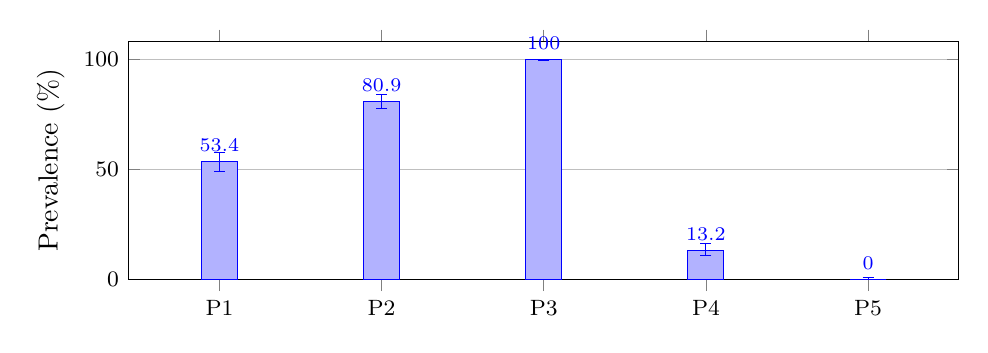
\begin{tikzpicture}
\begin{axis}[
  ybar, bar width=13pt,
  width=\linewidth, height=4.6cm,
  ymin=0, ymax=108, ylabel={Prevalence (\%)},
  symbolic x coords={P1,P2,P3,P4,P5},
  xtick=data, enlarge x limits=0.14,
  nodes near coords, nodes near coords align={vertical},
  every node near coord/.append style={font=\scriptsize},
  ymajorgrids, tick label style={font=\footnotesize},
]
% asymmetric explicit errors:  += (0, upper)  -= (0, lower)
\addplot+[error bars/.cd, y dir=both, y explicit]
coordinates {
  (P1,53.4)  += (0,4.2)  -= (0,4.3)
  (P2,80.9)  += (0,3.2)  -= (0,3.5)
  (P3,100.0) += (0,0.0)  -= (0,0.7)
  (P4,13.2)  += (0,3.2)  -= (0,2.6)
  (P5,0.0)   += (0,0.7)  -= (0,0.0)
};
\end{axis}
\end{tikzpicture}
\caption{Prevalence of cited verification weaknesses across 530 distinct
JWT-validating configurations, with Wilson 95\% confidence intervals.
P1 unbound audience; P2 no required claims; P3 no algorithm pinning \emph{in
configuration} (library-default caveat, \S\ref{sec:results}); P4 multi-issuer
(descriptive); P5 clock skew $>5$\,min (now read from Envoy
\texttt{clock\_skew\_seconds}; the widest observed is 60\,s). An independently
validated extractor; a hand-labelled gold standard is still pending
(\S\ref{sec:limitations}).}
\label{fig:prevalence}
\end{figure}

\noindent\textbf{Drift (RQ: how contracts change over time).}
Longitudinal analysis over commit history is future work. Today we validate the
drift \emph{classifier} on a 1{,}226-pair synthetic corpus at 100\% recall / 0\%
FPR, with mutation testing (24 mutants, 100\% killed) and a held-out adversarial
set at Youden 0.75. \gate{Drift in the wild, over real commit histories, is left to
the full study.}

\section{Limitations and threats to validity}\label{sec:limitations}
\textbf{Declared, not effective.} We measure the contract configuration declares,
not what the running verifier enforces. A configured check can still be skipped by
buggy verifier code, and a check absent from configuration can still hold because a
library default supplies it; conversely an implementation flaw (accepting
\texttt{alg=none}, RS/HS confusion) is invisible to us. We therefore report an
absent check as ``not set in configuration,'' not as a confirmed vulnerability, and
closing this gap needs live probing or a library-defaults database, which we leave
to future work. \textbf{Profile dependence.} Which checks are mandatory depends on
the token profile: audience and issuer validation are required for RFC~9068 access
tokens but optional for a bare RFC~7519 JWT, so an ``unbound audience'' is a
weakness only under a profile that requires binding; we measure the configured check
and name the profile where the corpus reveals it. \textbf{Templating:} $\approx$13\% of corpus files are
Helm-templated and $\approx$8\% carry kustomize/variable markers, so roughly one in
five configurations is under-resolved without rendering. \textbf{Selection bias:}
public configuration skews to samples, demos, and OSS and is not representative of
private enterprise deployments; this must be stated, not hidden. \textbf{Proxy
oracles:} \S\ref{sec:validation}'s recall/precision are automated approximations
pending human labels. \textbf{Ethics:} we use only public configuration, read
only; we do not probe third-party live endpoints and handle no real tokens;
identifiable high-severity findings follow responsible disclosure.

\section{Related work}\label{sec:related}
\noindent\textbf{In-the-wild web-authentication and SSO measurement.} The closest
line of work measures deployed authentication. Early studies inspect a small set of
sites by hand and show that SSO and OAuth failures are driven by deployment and
implementation choices rather than protocol flaws~\cite{authzmeas2012wangsignmein,authzmeas2012sunoauth}.
Later work makes this a population measurement: SSOScan automatically tests a fixed
catalog of five SSO vulnerabilities across the top 20{,}000 sites and finds that over
20\% of Facebook-SSO sites carry a serious flaw~\cite{authzmeas2014ssoscan}, and
subsequent studies measure sign-off and session handling, dual-window SSO, and SSO
adoption across the Tranco list~\cite{authzmeas2018singlesignoff,authzmeas2022distinct,authzmeas2023ssomonitor};
the OpenID Connect attack classes are systematized by Mainka et al.~\cite{authzmeas2017soksso}.
SSOScan is our closest methodological ancestor: automated detection of a fixed
weakness catalog over a crawled population. We keep that ambition but change the
object and the vantage point. We read the declared verification contract out of
static mesh and proxy configuration rather than driving a runtime login flow, which
reaches services no crawler can log into and separates what a service declares from
what it enforces.

\noindent\textbf{Large-scale misconfiguration measurement.} Our methodology follows
a well-established template: crawl a population, report the prevalence of a concrete
weakness, and quantify uncertainty. Studies of the HTTPS certificate ecosystem and
of Heartbleed turn repeated scans into a structured prevalence
picture~\cite{authzmeas2013httpsecosystem,authzmeas2014heartbleed}; the email-delivery
study measures adoption of \emph{declared} security policies (SPF, DKIM, DMARC)
across more than 700{,}000 servers~\cite{authzmeas2015emaildelivery}; and studies of
HTTPS adoption, Content Security Policy, CORS, and S3 buckets measure how a declared
per-service policy is set or fails at scale~\cite{authzmeas2017httpsadoption,authzmeas2016csp,authzmeas2018cors,authzmeas2018s3buckets}.
We adopt this template, including confidence intervals and a replication-style
validation of recall and precision, and apply it to a surface none of these touch,
the JWT authorization contract.

\noindent\textbf{IaC and configuration security.} Repository-mining studies quantify
security weaknesses in declarative infrastructure code: the Seven Sins study derives
smells from 1{,}726 scripts and counts occurrences across hundreds of
repositories~\cite{authzmeas2019sevensins}, replicated at larger scale and across
technologies~\cite{authzmeas2021iacreplication,authzmeas2022glitch}, and Kubernetes
security practice is systematized separately~\cite{authzmeas2020k8scommandments}.
Practitioner scanners (Checkov, KICS, Terrascan, Semgrep) and policy-as-code
engines~\cite{authzmeas2024checkov,authzmeas2024kics,authzmeas2024terrascan,authzmeas2024semgrep,authzmeas2024opa}
apply rule sets to individual files. These target generic hygiene (hard-coded
secrets, weak crypto) and check rules per file; we instead normalize heterogeneous
mesh and proxy configuration into one typed authorization contract per service and
measure its properties, and our negative control targets the attribution errors that
per-file pattern-matching is prone to.

\noindent\textbf{Formal analysis and config-as-contract.} A body of formal and
attack analysis establishes \emph{which} issuer, audience, algorithm, and endpoint
behaviours are load-bearing, for SAML, OAuth, and OpenID
Connect~\cite{authzmeas2008samlsso,authzmeas2012websanalysis,authzmeas2016oauthformal,authzmeas2017oidcformal};
the concrete JWT weaknesses we count (\texttt{alg=none}, RS/HS key confusion) are
documented by practitioners~\cite{authzmeas2015jwtlibs,authzmeas2024portswiggerjwt}
and codified in RFC~8725~\cite{rfc8725}. We cite these for the properties and then
measure how often deployments violate them rather than re-arguing relevance. The
idea of deriving a policy model from static configuration has a precedent in Batfish,
which parses heterogeneous device configuration into a vendor-independent model and
checks properties over it~\cite{authzmeas2015batfish}, and in ABAC policy
mining~\cite{authzmeas2015abacmining}; consumer-driven contract testing (Pact) shares
the ``contract'' framing~\cite{authzmeas2024pact}. None recovers a JWT authorization
contract or measures one across a population.

\noindent\textbf{Agent and MCP authorization.} Indirect prompt injection makes
token-scoped, verifiable authorization necessary for autonomous
agents~\cite{authzmeas2023promptinjection}, and recent measurements of live remote
MCP servers report widespread missing authentication and OAuth
flaws~\cite{authzmeas2026mcpauthmeas,authzmeas2026mcpexposed}. These show the same
population-measurement method reaching the agent frontier, where the declared-versus-effective
contract framing of this paper is the natural lens to carry forward.

\section{Future work}\label{sec:future}
Three extensions follow directly. (i) Pairing the static reading with live probing
would close the declared-vs-effective gap this paper is careful to leave open,
turning ``not set in configuration'' into a confirmed runtime behaviour. (ii) The
content-addressed contract makes \emph{drift} measurable over commit history: do
contracts widen more than they narrow, and are widenings tied to reviewable events?
(iii) The same instrument extends to the agent and MCP frontier, where OAuth/MCP
tokens carry the same issuer, audience, and claim checks on a faster-moving surface.

\section{Conclusion}
A service's decision to accept a token is configuration, declared across meshes,
proxies, and identity providers and rarely collected in one place. We make that
declared authorization contract an object that can be derived, measured, versioned,
and validated, we separate it from the effective enforcement that configuration
cannot show, and we measure it across 2{,}718 repositories with a methodology
honest about its own limits. The instrument and corpus are released so the
measurement is reproducible and extensible.

\section*{Ethics considerations}\label{sec:ethics}
This study measures only \emph{public} configuration, fetched read-only at pinned
commits, and never probes third-party live endpoints or handles real tokens; the
attack surface it characterises is exercised only against local, self-owned
negative-control fixtures. We report \emph{population} prevalence, never a verdict
on any single project, and we name no project as insecure. For any identifiable,
high-severity finding tied to a specific owner we follow coordinated responsible
disclosure before publication, allowing reasonable remediation time. The corpus
respects source licences (recorded per artifact) and robots/rate-limit norms of the
hosting platform. We see no human-subjects concerns; no personal data is collected.

\section*{Open science}\label{sec:openscience}
In keeping with open-science expectations, we release the discovery instrument, the
measurement harness (prevalence with Wilson CIs), the kind-aware validator, the
non-circular negative-control precision test, the analysis scripts, and the corpus
\emph{manifest} (repository + commit SHA + licence per artifact) so the measurement
is reproducible from public sources. \gate{At camera-ready we will add a DOI-pinned
archival snapshot and, where the venue offers it, Artifact-Evaluation ``Available'' and
``Reproduced'' badges.}

\section*{Artifact availability}\label{sec:artifact}
The instrument, harness, validator, negative-control test, and corpus manifest are
open source under the MIT licence. \gate{The archival DOI will be added at
camera-ready.}
 to bring
% back the loud [PENDING]/[NOTE] markers for internal tracking.
\ifdefined\ifsubmission\else\expandafter\newif\csname ifsubmission\endcsname\submissiontrue\fi
% \gate{...}: forward-looking text. Submission -> plain prose; draft -> [PENDING].
% Content is written to read as a finished future-work sentence either way.
\providecommand{\gate}[1]{\ifsubmission #1\else \textbf{[PENDING: #1]}\fi}
% \draftonly{...}: internal note. Submission -> nothing; draft -> [NOTE].
\providecommand{\draftonly}[1]{\ifsubmission\else \textbf{[NOTE: #1]}\fi}
% Let TeX relax line breaking on paragraphs with long unbreakable \texttt{} kind
% names (RequestAuthentication, AuthorizationPolicy) instead of overrunning the
% margin. Class-agnostic; applies under every venue wrapper.
\emergencystretch=3em

% The abstract lives in common/abstract.tex. acmart requires it BEFORE \maketitle,
% llncs/IEEEtran after, so an acmart wrapper \inputs it itself (and defines
% \keywayabstractdone); every other wrapper lets the body emit it here.
\ifdefined\keywayabstractdone\else\begin{abstract}
Whether a service accepts a JSON Web Token (JWT) is decided by configuration rather
than by application code: which token issuers it trusts, which audience a token must
name, which signing algorithms it accepts, and which claims it requires. In modern
deployments these settings are spread across a service mesh (e.g.\ Istio), an edge
proxy (e.g.\ Envoy), and an identity provider; they are rarely collected in one
place; and they change often, so a rotated signing key or a widened audience can
silently begin refusing valid requests or admitting tokens that should be rejected.
We call the resulting set of checks a service's implicit \emph{authorization
contract}. This paper makes that contract an object that can be \emph{derived} from
deployment configuration, measured, and compared across versions, and it separates
the \emph{declared} contract we extract from the \emph{effective} enforcement that
additionally depends on verifier code, library defaults, and software versions.

We derive authorization contracts from 2{,}718 public repositories and measure them
over 530 distinct JWT-validating configurations. None pins a signing algorithm in
configuration (each relies on a library default), 80.9\% require no claim beyond
issuer and audience, and 53.4\% leave the audience unbound; we report every figure
with a 95\% confidence interval. Because a measurement is only as sound as its
extractor, we validate discovery three ways and state the limit of each: recall
against an independent parse of the same configuration (issuers 96.0\%, audiences
98.2\%), precision against planted distractor values a correct extractor must
ignore, and a held-out split, labelled by an independent model that never sees the
extractor's output, that finds no over-attribution. We release the tool, the corpus
manifest, and the analysis.
\end{abstract}
\fi

\section{Introduction}
An engineer rotates a signing key on a Friday. No code changes; every test passes.
By Monday a downstream service is rejecting every valid user, because its verifier
cached the retired key longer than anyone realised. The same week, elsewhere, a
verifier quietly begins accepting a second audience nobody intended. Neither
failure lives in the code, and neither would be caught by reading it: both live in
the \emph{configuration} that actually decides whether a bearer token is accepted.

That configuration is an implicit specification: the issuers a verifier trusts,
the audiences it binds to, the algorithms it allows, the claims it requires, and
the JWKS behaviour of the library beneath it. We call it the \emph{authorization
contract}. It is spread across service meshes, proxies, identity providers, and
library defaults, it is almost never centralised, and it \emph{drifts}: a rotated
key, a widened audience, or a dropped claim turns valid users away (an outage) or
admits tokens that should be refused (a silent regression). As autonomous agents
begin carrying OAuth/MCP tokens on a user's behalf, the same contract now governs a
faster-moving, higher-stakes surface.

A caveat shapes the whole paper. What configuration states is the \emph{declared}
contract; whether a request is ultimately accepted is the \emph{effective}
behaviour, which also depends on the verifier's code, its library's defaults, and
its software version. A verifier may, for example, accept the \texttt{none}
algorithm because of an implementation flaw even where configuration says nothing,
and that is not visible in configuration at all. We measure the declared contract,
we say so throughout, and \S\ref{sec:background} and \S\ref{sec:limitations} make
the boundary between declared and effective explicit; where a declared value is
absent we distinguish ``not set in configuration'' from ``not enforced.''

This declared contract is where much of auth correctness is decided, and yet almost
nobody measures it at scale. Two kinds of tooling exist and neither answers ``what
do deployed authorization contracts look like across a population, and how healthy
are they?'' Static code scanners reason about source, not about which configured
verifier trusts which issuer; gateways and identity providers are the thing being
configured, so they do not tell an operator whether that configuration is healthy.

\noindent\textbf{Contributions.}
(i) We define the \emph{authorization contract} and give a method that derives it
from heterogeneous deployment configuration (Istio, Envoy, OIDC) with per-field
provenance and content-addressed versioning, separating the declared contract from
effective enforcement (\S\ref{sec:method}).
(ii) We measure how common concrete, normatively grounded weaknesses are across
2{,}718 public repositories and 530 JWT-validating configurations, with confidence
intervals and a co-occurrence analysis (\S\ref{sec:results}).
(iii) We give a validation methodology that is explicit about its own limits:
recall against an independent parse, a non-circular negative control for precision,
and a held-out over-attribution split, each with its failure mode stated
(\S\ref{sec:validation}).
(iv) We release the instrument, the corpus manifest, and the analysis so the study
is reproducible from public sources (\S\ref{sec:artifact}).

\section{Background}\label{sec:background}

\noindent\textbf{JWT verification.} A JSON Web Token is a signed statement of
claims: a header naming the signing algorithm, a payload of claims (including
\texttt{iss}, the issuer; \texttt{aud}, the intended audience; \texttt{exp}, the
expiry), and a signature. To accept a token, a verifier must (1) fetch the issuer's
public keys, in practice from a JSON Web Key Set (JWKS) endpoint, and verify the
signature; (2) check that \texttt{iss} is a trusted issuer; (3) check that
\texttt{aud} names this resource; (4) accept only an allow-list of signing
algorithms; and (5) enforce any additional required claims (roles, scopes, tenant).
Each step has a normative source. RFC~8725 (JSON Web Token Best Current Practices)
requires an explicit algorithm allow-list (\S3.1) and validation of all security
claims (\S3.9); RFC~9068 profiles JWT \emph{access tokens} and makes audience and
issuer validation mandatory for that profile; RFC~8707 (resource indicators) and
RFC~9728 (protected-resource metadata) bind a token to the resource it was minted
for. Which checks are mandatory therefore depends partly on the token profile in
use, a point we return to in \S\ref{sec:limitations}.

\noindent\textbf{Where the contract lives.} Few services implement these checks in
application code. In a service mesh the checks are declared as configuration and
enforced by a sidecar or gateway. Under Istio, a \texttt{RequestAuthentication}
resource declares the issuer, the JWKS source, and the accepted audiences, while an
\texttt{AuthorizationPolicy} declares required claims as \texttt{when} conditions on
\texttt{request.auth.claims[...]}; under Envoy, a \texttt{jwt\_authn} filter carries
the providers, audiences, and clock-skew tolerance. These resources usually live in
\emph{different files}, and the effective contract for one workload is their union.
Figure~\ref{fig:example} shows a minimal pair.

\begin{figure}[t]
\footnotesize
\begin{verbatim}
kind: RequestAuthentication      # issuer + audience
spec:
  selector: {matchLabels: {app: orders}}
  jwtRules:
  - issuer: "https://idp.example/realms/main"
    jwksUri: "https://idp.example/jwks.json"
    audiences: ["orders-api"]
---
kind: AuthorizationPolicy        # a required claim
spec:
  selector: {matchLabels: {app: orders}}
  rules:
  - when:
    - key: request.auth.claims[groups]
      values: ["ops"]
\end{verbatim}
\caption{The declared authorization contract for the \texttt{orders} workload,
spread across two resources: trust \texttt{idp.example}, require audience
\texttt{orders-api}, and require a \texttt{groups} claim of \texttt{ops}. No signing
algorithm is pinned, so the mesh applies its library default (\S\ref{sec:results}).}
\label{fig:example}
\end{figure}

\noindent\textbf{Declared vs.\ effective; terminology.} We measure the
\emph{declared} contract in resources like these. The \emph{effective} behaviour
can differ: a verifier might skip a check, honour a dangerous default, or carry an
implementation bug (accepting \texttt{alg=none}, confusing RS256 and HS256). Those
are code, not configuration, and outside the reach of a static reading; we flag the
absence of a configured check as ``not set in configuration,'' never as a confirmed
runtime vulnerability. We use \emph{consumer} for the verifying entity a contract
belongs to (an Istio workload, an Envoy route), and we restrict \emph{authorization
contract} to \emph{token validation} (is this token acceptable?), as distinct from
resource-level authorization (may this subject perform this action?), which is a
separate layer we do not measure.

\section{Deriving authorization contracts}\label{sec:method}
We derive one contract per \emph{consumer} (\S\ref{sec:background}) from the
configuration that governs it. Source-specific \emph{discoverers} parse each format
(Istio \texttt{RequestAuthentication} and \texttt{AuthorizationPolicy}, Envoy
\texttt{jwt\_authn}, and OIDC/Keycloak registries) into a common contract of
issuers, audiences, algorithms, required claims, and JWKS behaviour.

Deriving a contract is not a one-resource read, because the checks are split across
resources (\S\ref{sec:background}). For the pair in Figure~\ref{fig:example}, the
\texttt{RequestAuthentication} contributes the issuer, JWKS source, and audience,
and the \texttt{AuthorizationPolicy} contributes the required \texttt{groups} claim;
we join them by the workload they select (\texttt{app: orders}) into a single
consumer whose contract carries all three. Attribution follows the mesh's own
semantics: a selector-less policy applies to every workload in its namespace, and
in a namespace with a single JWT consumer a per-service claim policy attaches to
that consumer (the common edge-gateway pattern). The same join resolves audiences
declared in an \texttt{AuthorizationPolicy} condition on
\texttt{request.auth.audiences} rather than in the \texttt{RequestAuthentication}.

Every extracted field records \emph{provenance}: the source kind, the file
locator, and a confidence. Each measurement is therefore attributable to a line of
configuration and a human can check it (we use this in \S\ref{sec:validation}).
A library-defaults database records what a verifier does when configuration is
silent, kept separate from what configuration states so the two are never conflated.
Consumers are assembled into a content-addressed \texttt{ContractVersion}, which
makes change detection exact equality and lets us diff one deployment's contract
against another or against its own history.

\section{Corpus construction}\label{sec:corpus}
We crawl public GitHub read-only for real auth configuration (Istio
\texttt{RequestAuthentication}, Envoy \texttt{jwt\_authn}, Istio claim conditions),
recording repository, blob SHA, and licence for every artifact for reproducibility
and attribution. We fetch public repositories only, cap files per repository to
limit monorepo dominance, and analyse \emph{per repository} so a
\texttt{RequestAuthentication} and its \texttt{AuthorizationPolicy} (usually in
separate files) are resolved together while distinct repositories remain isolated.
Two cleaning steps address representativeness: we exclude tutorial/vendored copies
by path (matched against the full locator, so \texttt{testdata/}, \texttt{vendor/},
and \texttt{/e2e/} components are caught, not only basenames), and we deduplicate
identical configurations (a canonical sample pasted across repositories counts
once). The corpus is 5{,}214 files across 2{,}718 public repositories, yielding 778
JWT-validating configurations, or 530 after deduplication. \gate{A full study will
push the corpus further toward $10^4$ services, add OIDC/MCP sources, and report a
selection-bias analysis against the public-configuration population.}

\section{Validation methodology}\label{sec:validation}
Measurement is only as good as the extractor. We validate discovery three ways, for
recall, for precision, and for over-attribution, and are explicit about what each
can and cannot establish.

\noindent\textbf{Recall (kind-aware independent parse).} An independent YAML parse
of each repository yields the declared issuers/audiences/claims; we compare to what
discovery captured, per repository. The independent parser also
\emph{over-declares}: it scrapes \texttt{issuer:} keys and claim-like strings from
non-auth resources (a ConfigMap, an annotation). We therefore measure recall only
against values in \emph{genuine} auth resources (RequestAuthentication /
AuthorizationPolicy / Envoy JWT). Adjudicated recall is issuers 96.0\%, audiences
98.2\%, and claims 86.0\% (scoped to repositories where a JWT consumer exists;
claims declared in repositories whose RequestAuthentication is absent from the
corpus have no consumer to attach to). The adjudication removed 106 parser
over-declarations (65 issuers, 27 audiences, 14 claims), which both raises the
honest recall and demonstrates the proxy oracle is itself imperfect. The issuer
figure rose from an earlier 89.6\% once a document-splitting bug was fixed: a single
templated or malformed YAML document had been aborting the rest of its file, so the
earlier recall was depressed by the extractor, not by the corpus.

\noindent\textbf{Precision (non-circular negative control).} An independent-parse
oracle cannot honestly measure precision: it reads the same fields as the
extractor, so captures are almost always a subset and precision $\approx 100\%$
\emph{by construction}. We therefore use a negative control: configurations with
planted distractor values a correct discoverer must ignore: a commented-out
issuer, an \texttt{issuer:}/claim in a non-auth ConfigMap, a claim behind a
non-matching AuthorizationPolicy selector (the real attribution risk), and strings
in annotations. Result: 4 planted, 0 leaked, with real values still captured.

\noindent\textbf{Over-attribution (held-out split).} To measure how often discovery
\emph{adds} a value that is not really there, we take every captured/declared
disagreement, label each with an independent model that reads only the raw
configuration and never the extractor's output (so the grading is non-circular),
and split the labelled set 70/30 by repository so no repository informs both sides.
On the held-out test split, precision is 100\% and over-attribution is 0.0\% (0 of 6
captured-only values are spurious or mis-attributed); on the full labelled set,
precision 100\% and over-attribution 0.0\%. This split is what caught, and then
confirmed the fix for, an Envoy test-fixture leak and a claim mis-attribution during
development.

\noindent\textbf{Gold standard.} All three above are automated or model-assisted
proxies. For a population-level ground truth we draw a stratified random sample of
401 \mbox{(repo, field, value)} rows across the corpus, powered for a $\pm$1.8\%
precision and $\pm$2.4\% recall confidence interval, and have each adjudicated by
hand as real, correctly attributed, or spurious; a model drafts a first-pass label
that the human confirms or corrects, and a blind subset gives an un-anchored
inter-annotator agreement (Cohen's $\kappa$). \gate{We report the hand-validated
precision, recall, and $\kappa$ in the final version; the automated results above
are what the gold standard refines.}

\section{Results}\label{sec:results}
We report prevalence over the 530 deduplicated JWT-validating configurations, each
with a 95\% Wilson confidence interval (the Wilson interval is preferred over the
normal approximation for proportions near 0 or 1). These figures come from the
independently validated extractor of \S\ref{sec:validation}; the hand-validated
gold standard refines the \emph{validation} numbers, not the prevalence below.

\noindent\textbf{Prevalence.} Over 530 distinct JWT-validating configurations
(Wilson 95\% CIs): no algorithm pinning \emph{in configuration} 100\%
[99.3, 100]; no required claims 80.9\% [77.4, 84.1]; unbound audience 53.4\%
[49.1, 57.6]; multi-issuer trust 13.2\% [10.6, 16.4] (descriptive, not a weakness);
clock skew $>5$\,min 0.0\% [0.0, 0.7]. The algorithm-pinning figure reflects
reliance on the verifying \emph{library's default}, which configuration does not
restate. This is a static-vs-runtime gap, not a 100\% vulnerability rate; we report
it as ``not pinned in config.'' The clock-skew figure is now read directly from
Envoy \texttt{clock\_skew\_seconds} rather than assumed: of the configurations that
set it the widest is 60\,s, so the 0.0\% above the 5-minute threshold is measured,
not merely unobserved. The earlier draft's 42.2\% unbound-audience figure, over a
102-configuration pilot, rises to 53.4\% on this larger and more representative
corpus; the direction and the majority finding are unchanged.

\noindent\textbf{Co-occurrence.} Weaknesses travel together. No-required-claims and
no-algorithm-pinning co-occur in 80.9\% of configurations; unbound-audience with
no-algorithm-pinning in 53.4\%; unbound-audience with no-required-claims in 43.8\%
(lift $\approx$1.0, i.e. roughly independent rather than mutually reinforcing).

\noindent\textbf{Static/runtime frontier.} Four of the five check types are
conclusive from configuration alone; only algorithm pinning carries the
library-default caveat. Of 1{,}312 weakness flags raised, 782 (60\%) are
static-conclusive and 530 carry that caveat, quantifying how much of the contract a
purely static reading can settle.

% Prevalence figure (n=530 distinct JWT-validating configs, scaled corpus).
% Real values with Wilson 95% CIs (asymmetric). Requires pgfplots in the preamble
% (the wrappers add it). \input this inside the Results section.
\begin{figure}[t]
\centering
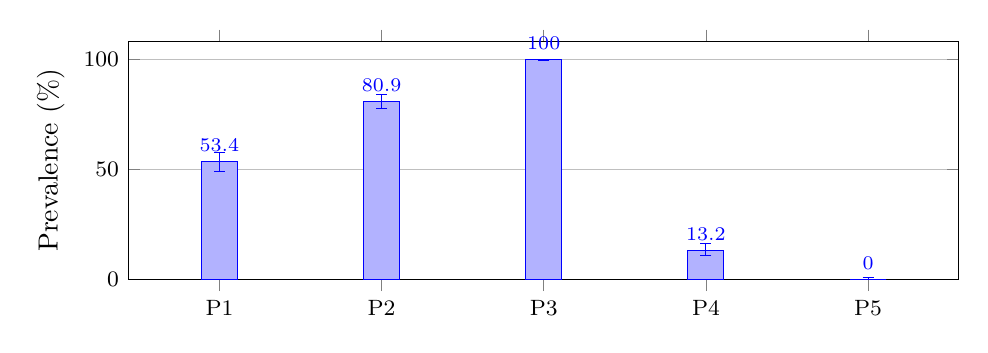
\begin{tikzpicture}
\begin{axis}[
  ybar, bar width=13pt,
  width=\linewidth, height=4.6cm,
  ymin=0, ymax=108, ylabel={Prevalence (\%)},
  symbolic x coords={P1,P2,P3,P4,P5},
  xtick=data, enlarge x limits=0.14,
  nodes near coords, nodes near coords align={vertical},
  every node near coord/.append style={font=\scriptsize},
  ymajorgrids, tick label style={font=\footnotesize},
]
% asymmetric explicit errors:  += (0, upper)  -= (0, lower)
\addplot+[error bars/.cd, y dir=both, y explicit]
coordinates {
  (P1,53.4)  += (0,4.2)  -= (0,4.3)
  (P2,80.9)  += (0,3.2)  -= (0,3.5)
  (P3,100.0) += (0,0.0)  -= (0,0.7)
  (P4,13.2)  += (0,3.2)  -= (0,2.6)
  (P5,0.0)   += (0,0.7)  -= (0,0.0)
};
\end{axis}
\end{tikzpicture}
\caption{Prevalence of cited verification weaknesses across 530 distinct
JWT-validating configurations, with Wilson 95\% confidence intervals.
P1 unbound audience; P2 no required claims; P3 no algorithm pinning \emph{in
configuration} (library-default caveat, \S\ref{sec:results}); P4 multi-issuer
(descriptive); P5 clock skew $>5$\,min (now read from Envoy
\texttt{clock\_skew\_seconds}; the widest observed is 60\,s). An independently
validated extractor; a hand-labelled gold standard is still pending
(\S\ref{sec:limitations}).}
\label{fig:prevalence}
\end{figure}

\noindent\textbf{Drift (RQ: how contracts change over time).}
Longitudinal analysis over commit history is future work. Today we validate the
drift \emph{classifier} on a 1{,}226-pair synthetic corpus at 100\% recall / 0\%
FPR, with mutation testing (24 mutants, 100\% killed) and a held-out adversarial
set at Youden 0.75. \gate{Drift in the wild, over real commit histories, is left to
the full study.}

\section{Limitations and threats to validity}\label{sec:limitations}
\textbf{Declared, not effective.} We measure the contract configuration declares,
not what the running verifier enforces. A configured check can still be skipped by
buggy verifier code, and a check absent from configuration can still hold because a
library default supplies it; conversely an implementation flaw (accepting
\texttt{alg=none}, RS/HS confusion) is invisible to us. We therefore report an
absent check as ``not set in configuration,'' not as a confirmed vulnerability, and
closing this gap needs live probing or a library-defaults database, which we leave
to future work. \textbf{Profile dependence.} Which checks are mandatory depends on
the token profile: audience and issuer validation are required for RFC~9068 access
tokens but optional for a bare RFC~7519 JWT, so an ``unbound audience'' is a
weakness only under a profile that requires binding; we measure the configured check
and name the profile where the corpus reveals it. \textbf{Templating:} $\approx$13\% of corpus files are
Helm-templated and $\approx$8\% carry kustomize/variable markers, so roughly one in
five configurations is under-resolved without rendering. \textbf{Selection bias:}
public configuration skews to samples, demos, and OSS and is not representative of
private enterprise deployments; this must be stated, not hidden. \textbf{Proxy
oracles:} \S\ref{sec:validation}'s recall/precision are automated approximations
pending human labels. \textbf{Ethics:} we use only public configuration, read
only; we do not probe third-party live endpoints and handle no real tokens;
identifiable high-severity findings follow responsible disclosure.

\section{Related work}\label{sec:related}
\noindent\textbf{In-the-wild web-authentication and SSO measurement.} The closest
line of work measures deployed authentication. Early studies inspect a small set of
sites by hand and show that SSO and OAuth failures are driven by deployment and
implementation choices rather than protocol flaws~\cite{authzmeas2012wangsignmein,authzmeas2012sunoauth}.
Later work makes this a population measurement: SSOScan automatically tests a fixed
catalog of five SSO vulnerabilities across the top 20{,}000 sites and finds that over
20\% of Facebook-SSO sites carry a serious flaw~\cite{authzmeas2014ssoscan}, and
subsequent studies measure sign-off and session handling, dual-window SSO, and SSO
adoption across the Tranco list~\cite{authzmeas2018singlesignoff,authzmeas2022distinct,authzmeas2023ssomonitor};
the OpenID Connect attack classes are systematized by Mainka et al.~\cite{authzmeas2017soksso}.
SSOScan is our closest methodological ancestor: automated detection of a fixed
weakness catalog over a crawled population. We keep that ambition but change the
object and the vantage point. We read the declared verification contract out of
static mesh and proxy configuration rather than driving a runtime login flow, which
reaches services no crawler can log into and separates what a service declares from
what it enforces.

\noindent\textbf{Large-scale misconfiguration measurement.} Our methodology follows
a well-established template: crawl a population, report the prevalence of a concrete
weakness, and quantify uncertainty. Studies of the HTTPS certificate ecosystem and
of Heartbleed turn repeated scans into a structured prevalence
picture~\cite{authzmeas2013httpsecosystem,authzmeas2014heartbleed}; the email-delivery
study measures adoption of \emph{declared} security policies (SPF, DKIM, DMARC)
across more than 700{,}000 servers~\cite{authzmeas2015emaildelivery}; and studies of
HTTPS adoption, Content Security Policy, CORS, and S3 buckets measure how a declared
per-service policy is set or fails at scale~\cite{authzmeas2017httpsadoption,authzmeas2016csp,authzmeas2018cors,authzmeas2018s3buckets}.
We adopt this template, including confidence intervals and a replication-style
validation of recall and precision, and apply it to a surface none of these touch,
the JWT authorization contract.

\noindent\textbf{IaC and configuration security.} Repository-mining studies quantify
security weaknesses in declarative infrastructure code: the Seven Sins study derives
smells from 1{,}726 scripts and counts occurrences across hundreds of
repositories~\cite{authzmeas2019sevensins}, replicated at larger scale and across
technologies~\cite{authzmeas2021iacreplication,authzmeas2022glitch}, and Kubernetes
security practice is systematized separately~\cite{authzmeas2020k8scommandments}.
Practitioner scanners (Checkov, KICS, Terrascan, Semgrep) and policy-as-code
engines~\cite{authzmeas2024checkov,authzmeas2024kics,authzmeas2024terrascan,authzmeas2024semgrep,authzmeas2024opa}
apply rule sets to individual files. These target generic hygiene (hard-coded
secrets, weak crypto) and check rules per file; we instead normalize heterogeneous
mesh and proxy configuration into one typed authorization contract per service and
measure its properties, and our negative control targets the attribution errors that
per-file pattern-matching is prone to.

\noindent\textbf{Formal analysis and config-as-contract.} A body of formal and
attack analysis establishes \emph{which} issuer, audience, algorithm, and endpoint
behaviours are load-bearing, for SAML, OAuth, and OpenID
Connect~\cite{authzmeas2008samlsso,authzmeas2012websanalysis,authzmeas2016oauthformal,authzmeas2017oidcformal};
the concrete JWT weaknesses we count (\texttt{alg=none}, RS/HS key confusion) are
documented by practitioners~\cite{authzmeas2015jwtlibs,authzmeas2024portswiggerjwt}
and codified in RFC~8725~\cite{rfc8725}. We cite these for the properties and then
measure how often deployments violate them rather than re-arguing relevance. The
idea of deriving a policy model from static configuration has a precedent in Batfish,
which parses heterogeneous device configuration into a vendor-independent model and
checks properties over it~\cite{authzmeas2015batfish}, and in ABAC policy
mining~\cite{authzmeas2015abacmining}; consumer-driven contract testing (Pact) shares
the ``contract'' framing~\cite{authzmeas2024pact}. None recovers a JWT authorization
contract or measures one across a population.

\noindent\textbf{Agent and MCP authorization.} Indirect prompt injection makes
token-scoped, verifiable authorization necessary for autonomous
agents~\cite{authzmeas2023promptinjection}, and recent measurements of live remote
MCP servers report widespread missing authentication and OAuth
flaws~\cite{authzmeas2026mcpauthmeas,authzmeas2026mcpexposed}. These show the same
population-measurement method reaching the agent frontier, where the declared-versus-effective
contract framing of this paper is the natural lens to carry forward.

\section{Future work}\label{sec:future}
Three extensions follow directly. (i) Pairing the static reading with live probing
would close the declared-vs-effective gap this paper is careful to leave open,
turning ``not set in configuration'' into a confirmed runtime behaviour. (ii) The
content-addressed contract makes \emph{drift} measurable over commit history: do
contracts widen more than they narrow, and are widenings tied to reviewable events?
(iii) The same instrument extends to the agent and MCP frontier, where OAuth/MCP
tokens carry the same issuer, audience, and claim checks on a faster-moving surface.

\section{Conclusion}
A service's decision to accept a token is configuration, declared across meshes,
proxies, and identity providers and rarely collected in one place. We make that
declared authorization contract an object that can be derived, measured, versioned,
and validated, we separate it from the effective enforcement that configuration
cannot show, and we measure it across 2{,}718 repositories with a methodology
honest about its own limits. The instrument and corpus are released so the
measurement is reproducible and extensible.

\section*{Ethics considerations}\label{sec:ethics}
This study measures only \emph{public} configuration, fetched read-only at pinned
commits, and never probes third-party live endpoints or handles real tokens; the
attack surface it characterises is exercised only against local, self-owned
negative-control fixtures. We report \emph{population} prevalence, never a verdict
on any single project, and we name no project as insecure. For any identifiable,
high-severity finding tied to a specific owner we follow coordinated responsible
disclosure before publication, allowing reasonable remediation time. The corpus
respects source licences (recorded per artifact) and robots/rate-limit norms of the
hosting platform. We see no human-subjects concerns; no personal data is collected.

\section*{Open science}\label{sec:openscience}
In keeping with open-science expectations, we release the discovery instrument, the
measurement harness (prevalence with Wilson CIs), the kind-aware validator, the
non-circular negative-control precision test, the analysis scripts, and the corpus
\emph{manifest} (repository + commit SHA + licence per artifact) so the measurement
is reproducible from public sources. \gate{At camera-ready we will add a DOI-pinned
archival snapshot and, where the venue offers it, Artifact-Evaluation ``Available'' and
``Reproduced'' badges.}

\section*{Artifact availability}\label{sec:artifact}
The instrument, harness, validator, negative-control test, and corpus manifest are
open source under the MIT licence. \gate{The archival DOI will be added at
camera-ready.}
 to bring
% back the loud [PENDING]/[NOTE] markers for internal tracking.
\ifdefined\ifsubmission\else\expandafter\newif\csname ifsubmission\endcsname\submissiontrue\fi
% \gate{...}: forward-looking text. Submission -> plain prose; draft -> [PENDING].
% Content is written to read as a finished future-work sentence either way.
\providecommand{\gate}[1]{\ifsubmission #1\else \textbf{[PENDING: #1]}\fi}
% \draftonly{...}: internal note. Submission -> nothing; draft -> [NOTE].
\providecommand{\draftonly}[1]{\ifsubmission\else \textbf{[NOTE: #1]}\fi}
% Let TeX relax line breaking on paragraphs with long unbreakable \texttt{} kind
% names (RequestAuthentication, AuthorizationPolicy) instead of overrunning the
% margin. Class-agnostic; applies under every venue wrapper.
\emergencystretch=3em

% The abstract lives in common/abstract.tex. acmart requires it BEFORE \maketitle,
% llncs/IEEEtran after, so an acmart wrapper \inputs it itself (and defines
% \keywayabstractdone); every other wrapper lets the body emit it here.
\ifdefined\keywayabstractdone\else\begin{abstract}
Whether a service accepts a JSON Web Token (JWT) is decided by configuration rather
than by application code: which token issuers it trusts, which audience a token must
name, which signing algorithms it accepts, and which claims it requires. In modern
deployments these settings are spread across a service mesh (e.g.\ Istio), an edge
proxy (e.g.\ Envoy), and an identity provider; they are rarely collected in one
place; and they change often, so a rotated signing key or a widened audience can
silently begin refusing valid requests or admitting tokens that should be rejected.
We call the resulting set of checks a service's implicit \emph{authorization
contract}. This paper makes that contract an object that can be \emph{derived} from
deployment configuration, measured, and compared across versions, and it separates
the \emph{declared} contract we extract from the \emph{effective} enforcement that
additionally depends on verifier code, library defaults, and software versions.

We derive authorization contracts from 2{,}718 public repositories and measure them
over 530 distinct JWT-validating configurations. None pins a signing algorithm in
configuration (each relies on a library default), 80.9\% require no claim beyond
issuer and audience, and 53.4\% leave the audience unbound; we report every figure
with a 95\% confidence interval. Because a measurement is only as sound as its
extractor, we validate discovery three ways and state the limit of each: recall
against an independent parse of the same configuration (issuers 96.0\%, audiences
98.2\%), precision against planted distractor values a correct extractor must
ignore, and a held-out split, labelled by an independent model that never sees the
extractor's output, that finds no over-attribution. We release the tool, the corpus
manifest, and the analysis.
\end{abstract}
\fi

\section{Introduction}
An engineer rotates a signing key on a Friday. No code changes; every test passes.
By Monday a downstream service is rejecting every valid user, because its verifier
cached the retired key longer than anyone realised. The same week, elsewhere, a
verifier quietly begins accepting a second audience nobody intended. Neither
failure lives in the code, and neither would be caught by reading it: both live in
the \emph{configuration} that actually decides whether a bearer token is accepted.

That configuration is an implicit specification: the issuers a verifier trusts,
the audiences it binds to, the algorithms it allows, the claims it requires, and
the JWKS behaviour of the library beneath it. We call it the \emph{authorization
contract}. It is spread across service meshes, proxies, identity providers, and
library defaults, it is almost never centralised, and it \emph{drifts}: a rotated
key, a widened audience, or a dropped claim turns valid users away (an outage) or
admits tokens that should be refused (a silent regression). As autonomous agents
begin carrying OAuth/MCP tokens on a user's behalf, the same contract now governs a
faster-moving, higher-stakes surface.

A caveat shapes the whole paper. What configuration states is the \emph{declared}
contract; whether a request is ultimately accepted is the \emph{effective}
behaviour, which also depends on the verifier's code, its library's defaults, and
its software version. A verifier may, for example, accept the \texttt{none}
algorithm because of an implementation flaw even where configuration says nothing,
and that is not visible in configuration at all. We measure the declared contract,
we say so throughout, and \S\ref{sec:background} and \S\ref{sec:limitations} make
the boundary between declared and effective explicit; where a declared value is
absent we distinguish ``not set in configuration'' from ``not enforced.''

This declared contract is where much of auth correctness is decided, and yet almost
nobody measures it at scale. Two kinds of tooling exist and neither answers ``what
do deployed authorization contracts look like across a population, and how healthy
are they?'' Static code scanners reason about source, not about which configured
verifier trusts which issuer; gateways and identity providers are the thing being
configured, so they do not tell an operator whether that configuration is healthy.

\noindent\textbf{Contributions.}
(i) We define the \emph{authorization contract} and give a method that derives it
from heterogeneous deployment configuration (Istio, Envoy, OIDC) with per-field
provenance and content-addressed versioning, separating the declared contract from
effective enforcement (\S\ref{sec:method}).
(ii) We measure how common concrete, normatively grounded weaknesses are across
2{,}718 public repositories and 530 JWT-validating configurations, with confidence
intervals and a co-occurrence analysis (\S\ref{sec:results}).
(iii) We give a validation methodology that is explicit about its own limits:
recall against an independent parse, a non-circular negative control for precision,
and a held-out over-attribution split, each with its failure mode stated
(\S\ref{sec:validation}).
(iv) We release the instrument, the corpus manifest, and the analysis so the study
is reproducible from public sources (\S\ref{sec:artifact}).

\section{Background}\label{sec:background}

\noindent\textbf{JWT verification.} A JSON Web Token is a signed statement of
claims: a header naming the signing algorithm, a payload of claims (including
\texttt{iss}, the issuer; \texttt{aud}, the intended audience; \texttt{exp}, the
expiry), and a signature. To accept a token, a verifier must (1) fetch the issuer's
public keys, in practice from a JSON Web Key Set (JWKS) endpoint, and verify the
signature; (2) check that \texttt{iss} is a trusted issuer; (3) check that
\texttt{aud} names this resource; (4) accept only an allow-list of signing
algorithms; and (5) enforce any additional required claims (roles, scopes, tenant).
Each step has a normative source. RFC~8725 (JSON Web Token Best Current Practices)
requires an explicit algorithm allow-list (\S3.1) and validation of all security
claims (\S3.9); RFC~9068 profiles JWT \emph{access tokens} and makes audience and
issuer validation mandatory for that profile; RFC~8707 (resource indicators) and
RFC~9728 (protected-resource metadata) bind a token to the resource it was minted
for. Which checks are mandatory therefore depends partly on the token profile in
use, a point we return to in \S\ref{sec:limitations}.

\noindent\textbf{Where the contract lives.} Few services implement these checks in
application code. In a service mesh the checks are declared as configuration and
enforced by a sidecar or gateway. Under Istio, a \texttt{RequestAuthentication}
resource declares the issuer, the JWKS source, and the accepted audiences, while an
\texttt{AuthorizationPolicy} declares required claims as \texttt{when} conditions on
\texttt{request.auth.claims[...]}; under Envoy, a \texttt{jwt\_authn} filter carries
the providers, audiences, and clock-skew tolerance. These resources usually live in
\emph{different files}, and the effective contract for one workload is their union.
Figure~\ref{fig:example} shows a minimal pair.

\begin{figure}[t]
\footnotesize
\begin{verbatim}
kind: RequestAuthentication      # issuer + audience
spec:
  selector: {matchLabels: {app: orders}}
  jwtRules:
  - issuer: "https://idp.example/realms/main"
    jwksUri: "https://idp.example/jwks.json"
    audiences: ["orders-api"]
---
kind: AuthorizationPolicy        # a required claim
spec:
  selector: {matchLabels: {app: orders}}
  rules:
  - when:
    - key: request.auth.claims[groups]
      values: ["ops"]
\end{verbatim}
\caption{The declared authorization contract for the \texttt{orders} workload,
spread across two resources: trust \texttt{idp.example}, require audience
\texttt{orders-api}, and require a \texttt{groups} claim of \texttt{ops}. No signing
algorithm is pinned, so the mesh applies its library default (\S\ref{sec:results}).}
\label{fig:example}
\end{figure}

\noindent\textbf{Declared vs.\ effective; terminology.} We measure the
\emph{declared} contract in resources like these. The \emph{effective} behaviour
can differ: a verifier might skip a check, honour a dangerous default, or carry an
implementation bug (accepting \texttt{alg=none}, confusing RS256 and HS256). Those
are code, not configuration, and outside the reach of a static reading; we flag the
absence of a configured check as ``not set in configuration,'' never as a confirmed
runtime vulnerability. We use \emph{consumer} for the verifying entity a contract
belongs to (an Istio workload, an Envoy route), and we restrict \emph{authorization
contract} to \emph{token validation} (is this token acceptable?), as distinct from
resource-level authorization (may this subject perform this action?), which is a
separate layer we do not measure.

\section{Deriving authorization contracts}\label{sec:method}
We derive one contract per \emph{consumer} (\S\ref{sec:background}) from the
configuration that governs it. Source-specific \emph{discoverers} parse each format
(Istio \texttt{RequestAuthentication} and \texttt{AuthorizationPolicy}, Envoy
\texttt{jwt\_authn}, and OIDC/Keycloak registries) into a common contract of
issuers, audiences, algorithms, required claims, and JWKS behaviour.

Deriving a contract is not a one-resource read, because the checks are split across
resources (\S\ref{sec:background}). For the pair in Figure~\ref{fig:example}, the
\texttt{RequestAuthentication} contributes the issuer, JWKS source, and audience,
and the \texttt{AuthorizationPolicy} contributes the required \texttt{groups} claim;
we join them by the workload they select (\texttt{app: orders}) into a single
consumer whose contract carries all three. Attribution follows the mesh's own
semantics: a selector-less policy applies to every workload in its namespace, and
in a namespace with a single JWT consumer a per-service claim policy attaches to
that consumer (the common edge-gateway pattern). The same join resolves audiences
declared in an \texttt{AuthorizationPolicy} condition on
\texttt{request.auth.audiences} rather than in the \texttt{RequestAuthentication}.

Every extracted field records \emph{provenance}: the source kind, the file
locator, and a confidence. Each measurement is therefore attributable to a line of
configuration and a human can check it (we use this in \S\ref{sec:validation}).
A library-defaults database records what a verifier does when configuration is
silent, kept separate from what configuration states so the two are never conflated.
Consumers are assembled into a content-addressed \texttt{ContractVersion}, which
makes change detection exact equality and lets us diff one deployment's contract
against another or against its own history.

\section{Corpus construction}\label{sec:corpus}
We crawl public GitHub read-only for real auth configuration (Istio
\texttt{RequestAuthentication}, Envoy \texttt{jwt\_authn}, Istio claim conditions),
recording repository, blob SHA, and licence for every artifact for reproducibility
and attribution. We fetch public repositories only, cap files per repository to
limit monorepo dominance, and analyse \emph{per repository} so a
\texttt{RequestAuthentication} and its \texttt{AuthorizationPolicy} (usually in
separate files) are resolved together while distinct repositories remain isolated.
Two cleaning steps address representativeness: we exclude tutorial/vendored copies
by path (matched against the full locator, so \texttt{testdata/}, \texttt{vendor/},
and \texttt{/e2e/} components are caught, not only basenames), and we deduplicate
identical configurations (a canonical sample pasted across repositories counts
once). The corpus is 5{,}214 files across 2{,}718 public repositories, yielding 778
JWT-validating configurations, or 530 after deduplication. \gate{A full study will
push the corpus further toward $10^4$ services, add OIDC/MCP sources, and report a
selection-bias analysis against the public-configuration population.}

\section{Validation methodology}\label{sec:validation}
Measurement is only as good as the extractor. We validate discovery three ways, for
recall, for precision, and for over-attribution, and are explicit about what each
can and cannot establish.

\noindent\textbf{Recall (kind-aware independent parse).} An independent YAML parse
of each repository yields the declared issuers/audiences/claims; we compare to what
discovery captured, per repository. The independent parser also
\emph{over-declares}: it scrapes \texttt{issuer:} keys and claim-like strings from
non-auth resources (a ConfigMap, an annotation). We therefore measure recall only
against values in \emph{genuine} auth resources (RequestAuthentication /
AuthorizationPolicy / Envoy JWT). Adjudicated recall is issuers 96.0\%, audiences
98.2\%, and claims 86.0\% (scoped to repositories where a JWT consumer exists;
claims declared in repositories whose RequestAuthentication is absent from the
corpus have no consumer to attach to). The adjudication removed 106 parser
over-declarations (65 issuers, 27 audiences, 14 claims), which both raises the
honest recall and demonstrates the proxy oracle is itself imperfect. The issuer
figure rose from an earlier 89.6\% once a document-splitting bug was fixed: a single
templated or malformed YAML document had been aborting the rest of its file, so the
earlier recall was depressed by the extractor, not by the corpus.

\noindent\textbf{Precision (non-circular negative control).} An independent-parse
oracle cannot honestly measure precision: it reads the same fields as the
extractor, so captures are almost always a subset and precision $\approx 100\%$
\emph{by construction}. We therefore use a negative control: configurations with
planted distractor values a correct discoverer must ignore: a commented-out
issuer, an \texttt{issuer:}/claim in a non-auth ConfigMap, a claim behind a
non-matching AuthorizationPolicy selector (the real attribution risk), and strings
in annotations. Result: 4 planted, 0 leaked, with real values still captured.

\noindent\textbf{Over-attribution (held-out split).} To measure how often discovery
\emph{adds} a value that is not really there, we take every captured/declared
disagreement, label each with an independent model that reads only the raw
configuration and never the extractor's output (so the grading is non-circular),
and split the labelled set 70/30 by repository so no repository informs both sides.
On the held-out test split, precision is 100\% and over-attribution is 0.0\% (0 of 6
captured-only values are spurious or mis-attributed); on the full labelled set,
precision 100\% and over-attribution 0.0\%. This split is what caught, and then
confirmed the fix for, an Envoy test-fixture leak and a claim mis-attribution during
development.

\noindent\textbf{Gold standard.} All three above are automated or model-assisted
proxies. For a population-level ground truth we draw a stratified random sample of
401 \mbox{(repo, field, value)} rows across the corpus, powered for a $\pm$1.8\%
precision and $\pm$2.4\% recall confidence interval, and have each adjudicated by
hand as real, correctly attributed, or spurious; a model drafts a first-pass label
that the human confirms or corrects, and a blind subset gives an un-anchored
inter-annotator agreement (Cohen's $\kappa$). \gate{We report the hand-validated
precision, recall, and $\kappa$ in the final version; the automated results above
are what the gold standard refines.}

\section{Results}\label{sec:results}
We report prevalence over the 530 deduplicated JWT-validating configurations, each
with a 95\% Wilson confidence interval (the Wilson interval is preferred over the
normal approximation for proportions near 0 or 1). These figures come from the
independently validated extractor of \S\ref{sec:validation}; the hand-validated
gold standard refines the \emph{validation} numbers, not the prevalence below.

\noindent\textbf{Prevalence.} Over 530 distinct JWT-validating configurations
(Wilson 95\% CIs): no algorithm pinning \emph{in configuration} 100\%
[99.3, 100]; no required claims 80.9\% [77.4, 84.1]; unbound audience 53.4\%
[49.1, 57.6]; multi-issuer trust 13.2\% [10.6, 16.4] (descriptive, not a weakness);
clock skew $>5$\,min 0.0\% [0.0, 0.7]. The algorithm-pinning figure reflects
reliance on the verifying \emph{library's default}, which configuration does not
restate. This is a static-vs-runtime gap, not a 100\% vulnerability rate; we report
it as ``not pinned in config.'' The clock-skew figure is now read directly from
Envoy \texttt{clock\_skew\_seconds} rather than assumed: of the configurations that
set it the widest is 60\,s, so the 0.0\% above the 5-minute threshold is measured,
not merely unobserved. The earlier draft's 42.2\% unbound-audience figure, over a
102-configuration pilot, rises to 53.4\% on this larger and more representative
corpus; the direction and the majority finding are unchanged.

\noindent\textbf{Co-occurrence.} Weaknesses travel together. No-required-claims and
no-algorithm-pinning co-occur in 80.9\% of configurations; unbound-audience with
no-algorithm-pinning in 53.4\%; unbound-audience with no-required-claims in 43.8\%
(lift $\approx$1.0, i.e. roughly independent rather than mutually reinforcing).

\noindent\textbf{Static/runtime frontier.} Four of the five check types are
conclusive from configuration alone; only algorithm pinning carries the
library-default caveat. Of 1{,}312 weakness flags raised, 782 (60\%) are
static-conclusive and 530 carry that caveat, quantifying how much of the contract a
purely static reading can settle.

% Prevalence figure (n=530 distinct JWT-validating configs, scaled corpus).
% Real values with Wilson 95% CIs (asymmetric). Requires pgfplots in the preamble
% (the wrappers add it). \input this inside the Results section.
\begin{figure}[t]
\centering
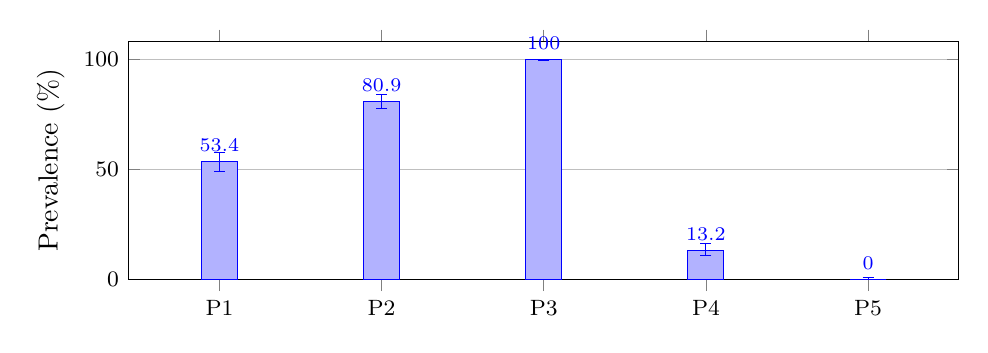
\begin{tikzpicture}
\begin{axis}[
  ybar, bar width=13pt,
  width=\linewidth, height=4.6cm,
  ymin=0, ymax=108, ylabel={Prevalence (\%)},
  symbolic x coords={P1,P2,P3,P4,P5},
  xtick=data, enlarge x limits=0.14,
  nodes near coords, nodes near coords align={vertical},
  every node near coord/.append style={font=\scriptsize},
  ymajorgrids, tick label style={font=\footnotesize},
]
% asymmetric explicit errors:  += (0, upper)  -= (0, lower)
\addplot+[error bars/.cd, y dir=both, y explicit]
coordinates {
  (P1,53.4)  += (0,4.2)  -= (0,4.3)
  (P2,80.9)  += (0,3.2)  -= (0,3.5)
  (P3,100.0) += (0,0.0)  -= (0,0.7)
  (P4,13.2)  += (0,3.2)  -= (0,2.6)
  (P5,0.0)   += (0,0.7)  -= (0,0.0)
};
\end{axis}
\end{tikzpicture}
\caption{Prevalence of cited verification weaknesses across 530 distinct
JWT-validating configurations, with Wilson 95\% confidence intervals.
P1 unbound audience; P2 no required claims; P3 no algorithm pinning \emph{in
configuration} (library-default caveat, \S\ref{sec:results}); P4 multi-issuer
(descriptive); P5 clock skew $>5$\,min (now read from Envoy
\texttt{clock\_skew\_seconds}; the widest observed is 60\,s). An independently
validated extractor; a hand-labelled gold standard is still pending
(\S\ref{sec:limitations}).}
\label{fig:prevalence}
\end{figure}

\noindent\textbf{Drift (RQ: how contracts change over time).}
Longitudinal analysis over commit history is future work. Today we validate the
drift \emph{classifier} on a 1{,}226-pair synthetic corpus at 100\% recall / 0\%
FPR, with mutation testing (24 mutants, 100\% killed) and a held-out adversarial
set at Youden 0.75. \gate{Drift in the wild, over real commit histories, is left to
the full study.}

\section{Limitations and threats to validity}\label{sec:limitations}
\textbf{Declared, not effective.} We measure the contract configuration declares,
not what the running verifier enforces. A configured check can still be skipped by
buggy verifier code, and a check absent from configuration can still hold because a
library default supplies it; conversely an implementation flaw (accepting
\texttt{alg=none}, RS/HS confusion) is invisible to us. We therefore report an
absent check as ``not set in configuration,'' not as a confirmed vulnerability, and
closing this gap needs live probing or a library-defaults database, which we leave
to future work. \textbf{Profile dependence.} Which checks are mandatory depends on
the token profile: audience and issuer validation are required for RFC~9068 access
tokens but optional for a bare RFC~7519 JWT, so an ``unbound audience'' is a
weakness only under a profile that requires binding; we measure the configured check
and name the profile where the corpus reveals it. \textbf{Templating:} $\approx$13\% of corpus files are
Helm-templated and $\approx$8\% carry kustomize/variable markers, so roughly one in
five configurations is under-resolved without rendering. \textbf{Selection bias:}
public configuration skews to samples, demos, and OSS and is not representative of
private enterprise deployments; this must be stated, not hidden. \textbf{Proxy
oracles:} \S\ref{sec:validation}'s recall/precision are automated approximations
pending human labels. \textbf{Ethics:} we use only public configuration, read
only; we do not probe third-party live endpoints and handle no real tokens;
identifiable high-severity findings follow responsible disclosure.

\section{Related work}\label{sec:related}
\noindent\textbf{In-the-wild web-authentication and SSO measurement.} The closest
line of work measures deployed authentication. Early studies inspect a small set of
sites by hand and show that SSO and OAuth failures are driven by deployment and
implementation choices rather than protocol flaws~\cite{authzmeas2012wangsignmein,authzmeas2012sunoauth}.
Later work makes this a population measurement: SSOScan automatically tests a fixed
catalog of five SSO vulnerabilities across the top 20{,}000 sites and finds that over
20\% of Facebook-SSO sites carry a serious flaw~\cite{authzmeas2014ssoscan}, and
subsequent studies measure sign-off and session handling, dual-window SSO, and SSO
adoption across the Tranco list~\cite{authzmeas2018singlesignoff,authzmeas2022distinct,authzmeas2023ssomonitor};
the OpenID Connect attack classes are systematized by Mainka et al.~\cite{authzmeas2017soksso}.
SSOScan is our closest methodological ancestor: automated detection of a fixed
weakness catalog over a crawled population. We keep that ambition but change the
object and the vantage point. We read the declared verification contract out of
static mesh and proxy configuration rather than driving a runtime login flow, which
reaches services no crawler can log into and separates what a service declares from
what it enforces.

\noindent\textbf{Large-scale misconfiguration measurement.} Our methodology follows
a well-established template: crawl a population, report the prevalence of a concrete
weakness, and quantify uncertainty. Studies of the HTTPS certificate ecosystem and
of Heartbleed turn repeated scans into a structured prevalence
picture~\cite{authzmeas2013httpsecosystem,authzmeas2014heartbleed}; the email-delivery
study measures adoption of \emph{declared} security policies (SPF, DKIM, DMARC)
across more than 700{,}000 servers~\cite{authzmeas2015emaildelivery}; and studies of
HTTPS adoption, Content Security Policy, CORS, and S3 buckets measure how a declared
per-service policy is set or fails at scale~\cite{authzmeas2017httpsadoption,authzmeas2016csp,authzmeas2018cors,authzmeas2018s3buckets}.
We adopt this template, including confidence intervals and a replication-style
validation of recall and precision, and apply it to a surface none of these touch,
the JWT authorization contract.

\noindent\textbf{IaC and configuration security.} Repository-mining studies quantify
security weaknesses in declarative infrastructure code: the Seven Sins study derives
smells from 1{,}726 scripts and counts occurrences across hundreds of
repositories~\cite{authzmeas2019sevensins}, replicated at larger scale and across
technologies~\cite{authzmeas2021iacreplication,authzmeas2022glitch}, and Kubernetes
security practice is systematized separately~\cite{authzmeas2020k8scommandments}.
Practitioner scanners (Checkov, KICS, Terrascan, Semgrep) and policy-as-code
engines~\cite{authzmeas2024checkov,authzmeas2024kics,authzmeas2024terrascan,authzmeas2024semgrep,authzmeas2024opa}
apply rule sets to individual files. These target generic hygiene (hard-coded
secrets, weak crypto) and check rules per file; we instead normalize heterogeneous
mesh and proxy configuration into one typed authorization contract per service and
measure its properties, and our negative control targets the attribution errors that
per-file pattern-matching is prone to.

\noindent\textbf{Formal analysis and config-as-contract.} A body of formal and
attack analysis establishes \emph{which} issuer, audience, algorithm, and endpoint
behaviours are load-bearing, for SAML, OAuth, and OpenID
Connect~\cite{authzmeas2008samlsso,authzmeas2012websanalysis,authzmeas2016oauthformal,authzmeas2017oidcformal};
the concrete JWT weaknesses we count (\texttt{alg=none}, RS/HS key confusion) are
documented by practitioners~\cite{authzmeas2015jwtlibs,authzmeas2024portswiggerjwt}
and codified in RFC~8725~\cite{rfc8725}. We cite these for the properties and then
measure how often deployments violate them rather than re-arguing relevance. The
idea of deriving a policy model from static configuration has a precedent in Batfish,
which parses heterogeneous device configuration into a vendor-independent model and
checks properties over it~\cite{authzmeas2015batfish}, and in ABAC policy
mining~\cite{authzmeas2015abacmining}; consumer-driven contract testing (Pact) shares
the ``contract'' framing~\cite{authzmeas2024pact}. None recovers a JWT authorization
contract or measures one across a population.

\noindent\textbf{Agent and MCP authorization.} Indirect prompt injection makes
token-scoped, verifiable authorization necessary for autonomous
agents~\cite{authzmeas2023promptinjection}, and recent measurements of live remote
MCP servers report widespread missing authentication and OAuth
flaws~\cite{authzmeas2026mcpauthmeas,authzmeas2026mcpexposed}. These show the same
population-measurement method reaching the agent frontier, where the declared-versus-effective
contract framing of this paper is the natural lens to carry forward.

\section{Future work}\label{sec:future}
Three extensions follow directly. (i) Pairing the static reading with live probing
would close the declared-vs-effective gap this paper is careful to leave open,
turning ``not set in configuration'' into a confirmed runtime behaviour. (ii) The
content-addressed contract makes \emph{drift} measurable over commit history: do
contracts widen more than they narrow, and are widenings tied to reviewable events?
(iii) The same instrument extends to the agent and MCP frontier, where OAuth/MCP
tokens carry the same issuer, audience, and claim checks on a faster-moving surface.

\section{Conclusion}
A service's decision to accept a token is configuration, declared across meshes,
proxies, and identity providers and rarely collected in one place. We make that
declared authorization contract an object that can be derived, measured, versioned,
and validated, we separate it from the effective enforcement that configuration
cannot show, and we measure it across 2{,}718 repositories with a methodology
honest about its own limits. The instrument and corpus are released so the
measurement is reproducible and extensible.

\section*{Ethics considerations}\label{sec:ethics}
This study measures only \emph{public} configuration, fetched read-only at pinned
commits, and never probes third-party live endpoints or handles real tokens; the
attack surface it characterises is exercised only against local, self-owned
negative-control fixtures. We report \emph{population} prevalence, never a verdict
on any single project, and we name no project as insecure. For any identifiable,
high-severity finding tied to a specific owner we follow coordinated responsible
disclosure before publication, allowing reasonable remediation time. The corpus
respects source licences (recorded per artifact) and robots/rate-limit norms of the
hosting platform. We see no human-subjects concerns; no personal data is collected.

\section*{Open science}\label{sec:openscience}
In keeping with open-science expectations, we release the discovery instrument, the
measurement harness (prevalence with Wilson CIs), the kind-aware validator, the
non-circular negative-control precision test, the analysis scripts, and the corpus
\emph{manifest} (repository + commit SHA + licence per artifact) so the measurement
is reproducible from public sources. \gate{At camera-ready we will add a DOI-pinned
archival snapshot and, where the venue offers it, Artifact-Evaluation ``Available'' and
``Reproduced'' badges.}

\section*{Artifact availability}\label{sec:artifact}
The instrument, harness, validator, negative-control test, and corpus manifest are
open source under the MIT licence. \gate{The archival DOI will be added at
camera-ready.}
